%%%%%%%%%%%%%%%%%%%%%%%%%%%%%%%%%%%%%%%%%%%%%%%%%%%%%%%
% A template for Wiley article submissions.
% Developed by Overleaf. 
%
% Please note that whilst this template provides a 
% preview of the typeset manuscript for submission, it 
% will not necessarily be the final publication layout.
%
% Usage notes:
% The "blind" option will make anonymous all author, affiliation, correspondence and funding information.
% Use "num-refs" option for numerical citation and references style.
% Use "alpha-refs" option for author-year citation and references style.

\documentclass[alpha-refs]{wiley-article-01g}
% \documentclass[blind,num-refs]{wiley-article}

% Add additional packages here if required
\usepackage{siunitx}
\usepackage{float}

% For figures

\usepackage{graphics}

%For captions 
\usepackage[labelfont=bf,justification=centering]{caption}
\usepackage[font=small,labelfont=bf]{subcaption}
\captionsetup[sub]{font=small,labelfont={bf,sf}}

%% For figures numbered by section
\usepackage{chngcntr}
\counterwithin{figure}{section}
\counterwithin{table}{section}

%% Additional links for hyperref
\usepackage[unicode=true,pdfusetitle,
 bookmarks=true,bookmarksnumbered=true,bookmarksopen=true,bookmarksopenlevel=2,
 breaklinks=false,pdfborder={0 0 1},backref=false,colorlinks=false]
 {hyperref}
\hypersetup{pdfstartview={XYZ null null 1}}


%% For fillers
\usepackage{lipsum}

%% For references 
\usepackage[backend=bibtex,
			natbib=true, 
			style=chicago-authordate]{biblatex}
\addbibresource{Returns.bib}

%% For landscape pages 

\usepackage{lscape}

%%%%%%%%#################################################################################%%%%%%%%%%%%%%%%%%%%%%%%%%%%%

% Update article type if known
\papertype{WORLD BANK EDUCATION GLOBAL PRACTICE}
% Include section in journal if known, otherwise delete
\paperfield{Russian Federation: Analytical Services and Advisory Activity: 
P170978}

\title{Returns to Education in the Russian Federation: Some New Estimates}

% List acknowledgments here.
\fundinginfo{Thanks are due to the Higher School of Economics, Moscow for making the Russian Longitudinal Monitoring Study (RLMS) Household data readily available for researchers around the world. The code used for this paper is made freely available for all researchers at \url{https://bitbucket.org/zagamog/edreru/src/master/}}

% Include full author names and degrees, when required by the journal.
% Use the \authfn to add symbols for additional footnotes and present addresses, if any. Usually start with 1 for notes about author contributions; then continuing with 2 etc if any author has a different present address.

\author[*]{Harry Patrinos}
\author[*]{\hspace{-1em}Suhas Parandekar}
\author[*]{\hspace{-1em}Ekaterina Melianova}
\author[*]{\hspace{-1em}Art\"{e}m Volgin}

% List abbreviations here, if any. Please note that it is preferred that abbreviations be defined at the first instance they appear in the text, rather than creating an abbreviations list.
\acks{\begin{normalsize}
\emph{Country Director:} Renaud Seligman; \emph{Regional Director:} Fadia Saadah; \emph{Practice Manager:} Harry Patrinos; \emph{Program Leader:} Dorota Nowak; \emph{Peer Reviewers}: Cristian Aedo; Ruslan Yemtsov; Husein Abdul-Hamid; \emph{Team members:} Polina Zavalina; Zhanna Terlyga. Thanks to seminar participants at the World Bank Moscow office on Jan. 29, 2020 for useful feedback. Any errors are a responsibility of the authors.
\end{normalsize}
\vspace{-0.2in}}

%\contrib[\authfn{1}]{Equally contributing authors.}

% Include full affiliation details for all authors
\affil[*]{Education Global Practice, Europe and Central Asia}

%\corraddress{Author One PhD, Department, Institution, City, State or Province, Postal Code, Country}
\corremail{sparandekar@worldbank.org}

%\presentadd[\authfn{2}]{Department, Institution, City, State or Province, Postal Code, Country}

% Include the name of the author that should appear in the running header
\runningauthor{P170978: WP01 - Returns to Education in the Russian Federation: Some New Estimates}

\begin{document}

\maketitle

\begin{abstract}
	
\vspace{.5em} \today	

\noindent This paper presents new estimates of the returns to education in 
the Russian Federation. Private returns to education are three times 
greater for higher education compared to vocational education, and the 
returns to education for females are higher than for males. Returns for 
females show an inverse U-shaped curve over the past two decades. Female 
education is a policy priority and there is a need to investigate the labor 
market relevance of vocational education. Higher education may have reached 
an expansion limit and it may be necessary to investigate options for 
increasing the productivity of schooling.

% Please include a maximum of seven keywords
\keywords{Returns to Education, Russian Federation \emph{JEL Codes: I26, 
I28, J16}}
\end{abstract}




\section{Motivation}

\begin{em}``How Wealthy is Russia?''\end{em} \hspace{-0.10em}is a recently published World Bank report that analyzed the human, natural, and produced capital of the Russian Federation \parencite{Naikal2019}. Human capital only accounts for 46\% of total wealth in Russia, as compared to the OECD average of 70\%.  The report showed that even as growth rates of per capita wealth were ten times higher in Russia as compared to the OECD, the gap in levels with OECD is still very wide. The per capita human capital wealth level on average for the OECD in 2014 was about USD 500,000 - five times that of Russia's 95,000 (measured in 2014 dollars). In order to catch up with the OECD, the returns to education in Russia will need to be increased. This paper presents the first in a series of papers on returns to education that will be instrumental in generating policy recommendations to improve the share of human capital as part of Russia's wealth. This paper examines the trends in returns to education in the Russian Federation using a common methodology used for more than 100 countries \parencite{Montenegro_Patrinos2014,Psacharopoulos_Patrinos2018}.  

\vspace{-0.2in}

\begin{center}
	\begin{figure}[htbp!]
\begin{minipage}[b]{1\linewidth}
			\centering
			\hspace*{-0.7in}
			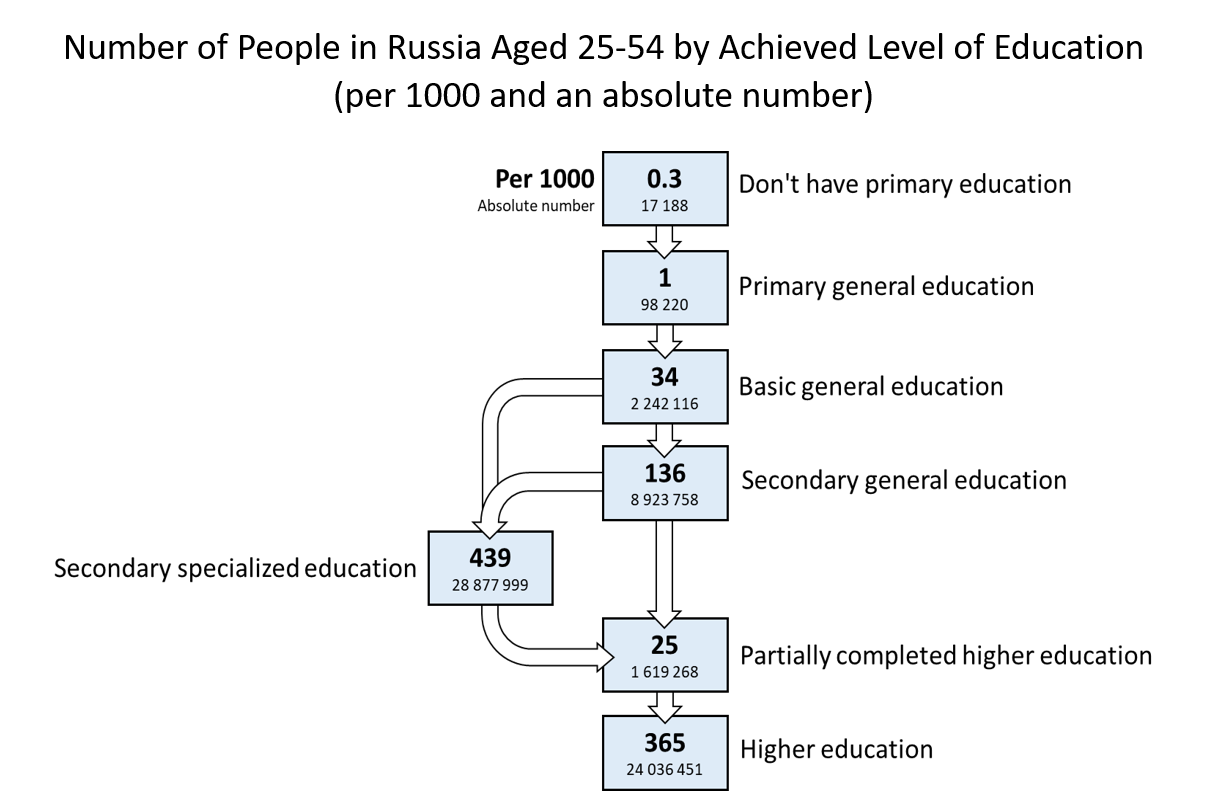
\includegraphics[width=5in]{graph_1c.png}
			% plot 1
		\end{minipage}
			\caption{Labor Force Distribution by Educational Level (Rosstat)}\label{fig:1.1a}
	\end{figure}
\end{center}


\vspace{-2em}


Figure \ref{fig:1.1a} indicates the educational attainment of the population segment 25 to 54 years, which is the age group for which Rosstat provides this information. Figure \ref{fig:1.1a}  shows less than 14\% of the labor force with a final attainment of secondary general education (academic High School) - the main choice is between vocational education (nearly 45\%) and university education (about 40\%). It is a well-known fact that on cognitive attainment at Grade 9, Russian students are already at par with OECD students (PISA scores are designed with an OECD mean of 500); what comes in later education levels and the labor market is the crucial issue for convergence with OECD on human capital wealth levels. 

A detailed analysis of the returns to education in the Russian Federation will provide insights into the stylized facts mentioned above. Together with other research being implemented by the World Bank and by other researchers, the purpose of this analysis is to come up with a set of evidence-based policy recommendations to enhance the human capital wealth of the Russian Federation. 

In this paper we report on an estimate of the private rate of return to 
investment in education in the Russian Federation. Human capital, or the 
stock of skills that is possessed by the labor force, is pivotal in 
enabling countries and individuals to flourish in a multifaceted, 
increasingly comprehensive, interrelated, and rapidly changing society 
\parencite{Schultz1972,Mincer1974,Heckman2003,Becker2009,Broecke2015}. The 
returns to investment in education have been a popular empirical analysis 
in research to study the relationship between schooling and earnings. 
Private returns can also explain the private demand for education. The 
literature suggests that each additional year of schooling produces a 
private (that is, individual) rate of return to schooling of about 8\% to 
9\%  a year 
\parencite{Psacharopoulos_Patrinos2018,Montenegro_Patrinos2014}. Globally, 
the returns to tertiary education are highest, followed by primary and then 
secondary schooling; this represents a significant reversal from many 
studies' prior results. Policy makers can learn much from Mincerian 
results; for instance, further expansion of university education appears to 
be very worthwhile for the individual, meaning that governments need to 
find ways to make financing more readily available, and that high rates of 
return are found through investment in girls' education.

\section{Literature Review}

In a worldwide perspective, the latest findings on returns to education can be condensed to the following \parencite{Psacharopoulos_Patrinos2018}: (1) overall, an amplified share of workers with tertiary education at the labor market has not reduced the magnitude of returns on the investment due to ``skill-biasedness'' of the technological progress boosting the demand for higher skills; (2) low- and middle-income regions are characterized by the largest returns (except for the Middle East and North Africa, with the lowest returns); (3) the private returns to education for women outstrip those for men by roughly two percentage points; (4) private sector employees receive greater returns than those working in the public sector; (5) social returns to education are negatively associated with a country's level of economic development and education level; and (6) on average, there is a growing trend in returns to higher education.

A separate, albeit scarce in terms of quantity, quality, and reliability, corpus of research focused on the Russian\slash USSR case. In the USSR during the period before education reforms the rates of return to schooling were strikingly low: 2-3\% for secondary and 5\% for higher education levels \parencite{Graeser1988}. Low returns to human capital were in line with a planned economy offering free education, centralized allocation of labor, and the ideology of proletariat superiority; a similar picture was observed in other (at the time) socialist countries (see, for example, \cite{Munich2005}).

However, an earlier attempt to establish the contribution of education to productivity took place during Soviet times. Strumilin showed that those who were more educated contributed more.  He even calculated earnings benefits, and though his calculations did not discount earnings, the estimates of the returns were high, at about 17 \% in 1919 \parencite{Strumilin1924}. 

A group of scholars reported that during the transition period from a planned to market economy in Russia rates of returns to schooling rose sharply \parencite{Brainerd1998,Clark2003,Vernon2002}. The upsurge in wage premiums to education (especially university education) was asserted to be a pivotal factor that exacerbated wage dispersion: salaries of highly skilled and trained workers had gone up in absolute terms and compared to less-educated workers \parencite{Fleisher2005}. However, returns to schooling declined for those people who took advantage of higher education expansion in a post-communist Russia (1990-2005) in comparison to youths who obtained university degrees in the preceding periods \parencite{Kyui2016}. One researcher exploited data about the average education level at the end of a Soviet period as an instrument and inferred that the growth in the proportion of city dwellers with university degree was associated with a rise in the wages of  city residents \parencite{ Muravyev2008}.
Despite enhancements in premiums to tertiary (professional and higher) education in the Russian Federation at the beginning of the 2000s, the labor market was shown to be different from that of developed countries. Comparing Russia with France, the existence of a vertical education-occupation mismatch in Russia was demonstrated \parencite{Kyui2010}. A recent paper claims that horizontal education-job mismatch negatively impacts upon the earnings of university graduates in all fields except for the lowest-paid ones \parencite{Rudakov2019}. Studies also suggest that education-job mismatch during studentship for individuals obtaining vocational education is "penalizing": combining studies with a job unrelated to a person's specialty entails a mismatch after his/her graduation \parencite{Dudyrev2018}.

Another research line ascertained that during the transition returns to education in Russia were not rising and remained among the lowest in the world \parencite{Cheidvasser2007}. The contradiction with previous inferences and reasoning was explained by the omitted variable bias: past researchers did not account for regional covariates and rural residence, thus overstating the returns. It was highlighted that the excess of well-educated workers seemed to be the main underpinning factor of wage differentials in Russia after the dissolution of the Soviet Union. Subsequently, Calvo et al. (2015) provide evidence of a reduction in skill premiums in Russia during the 2002 - 2012 period that was claimed to be one of the most relevant underlying forces explaining a deceleration in trends of widening wage inequality \parencite{Calvo2015}. Belskaya et al. (2014) evaluated a large-scale college expansion in Russia after the breakdown of the Soviet Union \parencite{Belskaya2014}. Among the key conclusions is that as the number of university campuses grew, individuals with low returns to schooling grew as well. But for a marginal person, who switched into a treatment group as a result of new campuses opening, the total gains from attending a college are considerable and positive. Furthermore, the scholars found that students with higher returns are attracted more intensively by new campuses opened in constrained municipalities (small non-capital cities or those lacking higher education institutions before college expansion) in comparison to the unconstrained ones. Like the global patterns, studies in Russia have shown that in the post-Soviet decade, workers hired in firms controlled\slash owned by private organizations\slash individuals, retained a marked premium to education in contrast to workers employed in state companies. This is rooted in a greater flexibility of private firms, enabling them to overcome restrictions caused by the rigidity of state wages, hence leading to higher returns to schooling \parencite{Clark2003}. \cite{Borisov2007} was among the first who employed cohort analysis, using Mincerian wage equation for the Russian data, and found evidence favoring the existence of a powerful vintage effect (especially for men) in the Russian labor market during the transition period: consecutive cohorts were paid more than the previous ones, keeping educational achievements constant; this phenomenon was entrenched in the specificity of a Soviet system, encouraging the pursuit of communist interests through extensive propaganda.
A source of heterogeneity in rates of returns to education in Russia hails from gender differences, just like the patterns observed globally: women received higher returns to higher education than men (e.g., \cite{Cheidvasser2007}; \cite{Lukyanova2010}). By the end of the first decade of the 21st century, some scholars detected positive changes concerning tertiary education in Russia (and other BRIC countries): payoff rates to university completion have generally magnified relative to the rates in lower levels of education and were higher than returns to secondary schooling \parencite{Carnoy2012}. This runs counter to the logic of capital theory, implying a decline in the rank order of returns with education level, which should hold with a country's economic advancement. Private rate of returns, even accounting for tuition cost, in Russia are especially high in business\slash economics as a field of study \parencite{Carnoy2012}. Additionally, rates of returns to vocational education were found to be lower than payoffs to tertiary education \parencite{Borisov2007}. In a recent paper, \cite{Gimpelson2019} argues that the labor market in Russia might be at risk of over-education, which leads to a reduction in educational premiums.

 
\section{Data}

In this paper we use the Russian Longitudinal Monitoring Survey (RLMS) - the only representative Russian survey with a sizable panel component allowing for dynamic analysis \parencite{Kozyreva2016}. The data are notable for their reliability, diversity, and applicability to a variety of research questions. The RLMS embraces information on people's income and expenditure structure, their material well-being, educational and occupational behavior, health state and nutrition, migration, etc.  RLMS sampling procedures have been thoroughly and extensively described elsewhere \parencite{Kozyreva2016}. The present research uses all 23 waves (1994 - 2018) that are available as of \today. Two years (1997 and 1999) are missing in the data because data was not collected in those years due to funding problems. The sub-sample selected for empirical investigation in this paper consists of working individuals aged 25-64 who are out of school and have positive labor market experience and income. 
\\

Table \ref{tab:1.1} shows descriptive statistics for the key variables under focus and sample sizes by years. The average years of experience is relatively stable over time, years of education slightly go up with higher education level becoming increasingly popular in Russia just as the proportion with vocational education declines. 

\begin{table}[ht]
	\centering
	\caption{Descriptive Statistics, RLMS}
	\label{tab:5.1}	
	\resizebox{\textwidth}{!}{
	\begin{tabular}{lcccccccccc}
\hline
 &  &  &  &  &  &  &  & \multicolumn{3}{c}{Education} \\ 
 &  & \multicolumn{2}{c}{Wage} & \multicolumn{2}{c}{Experience} & \multicolumn{2}{c}{Education_years} & Secondary & Vocational & \multicolumn{1}{c}{Higher} \\ 
Year  & N & Mean & SD & Mean & SD & Mean & SD & Percent & Percent & \multicolumn{1}{c}{Percent} \\ 
\hline
1994  & $3204$ & $266012.4$ & $339748.4$ & $\phantom{0000}22.5$ & $\phantom{0000}10.6$ & $\phantom{0000}12.4$ & $\phantom{00000}2.7$ & $\phantom{0000}21.3$ & $\phantom{0000}47.8$ & $\phantom{0000}25.9$ \\
1995  & $2792$ & $546812.3$ & $613489.6$ & $\phantom{0000}22.5$ & $\phantom{0000}10.4$ & $\phantom{0000}12.5$ & $\phantom{00000}2.5$ & $\phantom{0000}21.5$ & $\phantom{0000}46.1$ & $\phantom{0000}28.8$ \\
1996  & $2355$ & $803428.5$ & $993792.6$ & $\phantom{0000}22.3$ & $\phantom{0000}10.3$ & $\phantom{0000}12.6$ & $\phantom{00000}2.5$ & $\phantom{0000}19.2$ & $\phantom{0000}47.1$ & $\phantom{0000}30.7$ \\
1998  & $3186$ & $\phantom{000}895.2$ & $\phantom{000}943.0$ & $\phantom{0000}22.9$ & $\phantom{0000}10.2$ & $\phantom{0000}12.5$ & $\phantom{00000}2.4$ & $\phantom{0000}19.3$ & $\phantom{0000}50.7$ & $\phantom{0000}27.6$ \\
2000  & $3282$ & $\phantom{00}1807.6$ & $\phantom{00}2549.9$ & $\phantom{0000}22.7$ & $\phantom{0000}10.3$ & $\phantom{0000}12.6$ & $\phantom{00000}2.3$ & $\phantom{0000}19.9$ & $\phantom{0000}50.3$ & $\phantom{0000}27.9$ \\
2001  & $3659$ & $\phantom{00}2664.4$ & $\phantom{00}2838.6$ & $\phantom{0000}22.3$ & $\phantom{0000}10.1$ & $\phantom{0000}12.7$ & $\phantom{00000}2.3$ & $\phantom{0000}19.5$ & $\phantom{0000}48.6$ & $\phantom{0000}30.6$ \\
2002  & $3853$ & $\phantom{00}3595.9$ & $\phantom{00}4299.0$ & $\phantom{0000}22.3$ & $\phantom{0000}10.2$ & $\phantom{0000}12.7$ & $\phantom{00000}2.2$ & $\phantom{0000}19.1$ & $\phantom{0000}49.3$ & $\phantom{0000}30.5$ \\
2003  & $3900$ & $\phantom{00}4354.6$ & $\phantom{00}4002.5$ & $\phantom{0000}22.3$ & $\phantom{0000}10.2$ & $\phantom{0000}12.8$ & $\phantom{00000}2.2$ & $\phantom{0000}18.9$ & $\phantom{0000}49.0$ & $\phantom{0000}31.3$ \\
2004  & $3994$ & $\phantom{00}5361.3$ & $\phantom{00}4913.0$ & $\phantom{0000}22.1$ & $\phantom{0000}10.3$ & $\phantom{0000}12.8$ & $\phantom{00000}2.2$ & $\phantom{0000}18.3$ & $\phantom{0000}50.1$ & $\phantom{0000}31.0$ \\
2005  & $3937$ & $\phantom{00}6623.7$ & $\phantom{00}5714.6$ & $\phantom{0000}22.2$ & $\phantom{0000}10.5$ & $\phantom{0000}12.8$ & $\phantom{00000}2.2$ & $\phantom{0000}18.3$ & $\phantom{0000}49.4$ & $\phantom{0000}31.9$ \\
2006  & $4837$ & $\phantom{00}8080.8$ & $\phantom{00}6577.3$ & $\phantom{0000}22.3$ & $\phantom{0000}10.5$ & $\phantom{0000}12.8$ & $\phantom{00000}2.3$ & $\phantom{0000}17.9$ & $\phantom{0000}50.7$ & $\phantom{0000}30.9$ \\
2007  & $4766$ & $\phantom{00}9655.1$ & $\phantom{00}7128.8$ & $\phantom{0000}22.5$ & $\phantom{0000}10.6$ & $\phantom{0000}12.8$ & $\phantom{00000}2.3$ & $\phantom{0000}18.4$ & $\phantom{0000}49.9$ & $\phantom{0000}31.3$ \\
2008  & $4844$ & $\phantom{0}12787.8$ & $\phantom{0}10766.8$ & $\phantom{0000}22.6$ & $\phantom{0000}10.8$ & $\phantom{0000}12.9$ & $\phantom{00000}2.3$ & $\phantom{0000}17.8$ & $\phantom{0000}47.7$ & $\phantom{0000}34.2$ \\
2009  & $4818$ & $\phantom{0}13343.8$ & $\phantom{0}10408.6$ & $\phantom{0000}22.5$ & $\phantom{0000}11.0$ & $\phantom{0000}12.9$ & $\phantom{00000}2.3$ & $\phantom{0000}16.6$ & $\phantom{0000}47.7$ & $\phantom{0000}35.5$ \\
2010  & $7360$ & $\phantom{0}14742.7$ & $\phantom{0}12579.2$ & $\phantom{0000}22.6$ & $\phantom{0000}11.1$ & $\phantom{0000}13.0$ & $\phantom{00000}2.3$ & $\phantom{0000}16.9$ & $\phantom{0000}48.0$ & $\phantom{0000}34.9$ \\
2011  & $7197$ & $\phantom{0}16190.1$ & $\phantom{0}12853.0$ & $\phantom{0000}22.5$ & $\phantom{0000}11.1$ & $\phantom{0000}13.0$ & $\phantom{00000}2.3$ & $\phantom{0000}17.9$ & $\phantom{0000}46.8$ & $\phantom{0000}35.1$ \\
2012  & $7461$ & $\phantom{0}18844.4$ & $\phantom{0}15104.2$ & $\phantom{0000}22.5$ & $\phantom{0000}11.2$ & $\phantom{0000}12.9$ & $\phantom{00000}2.4$ & $\phantom{0000}18.2$ & $\phantom{0000}45.8$ & $\phantom{0000}35.8$ \\
2013  & $7346$ & $\phantom{0}20567.1$ & $\phantom{0}16404.0$ & $\phantom{0000}22.5$ & $\phantom{0000}11.2$ & $\phantom{0000}13.0$ & $\phantom{00000}2.3$ & $\phantom{0000}17.0$ & $\phantom{0000}46.7$ & $\phantom{0000}36.1$ \\
2014  & $6161$ & $\phantom{0}22733.9$ & $\phantom{0}17280.3$ & $\phantom{0000}22.3$ & $\phantom{0000}11.1$ & $\phantom{0000}13.1$ & $\phantom{00000}2.3$ & $\phantom{0000}16.5$ & $\phantom{0000}45.7$ & $\phantom{0000}37.6$ \\
2015  & $6236$ & $\phantom{0}23531.6$ & $\phantom{0}16965.8$ & $\phantom{0000}22.2$ & $\phantom{0000}11.2$ & $\phantom{0000}13.2$ & $\phantom{00000}2.3$ & $\phantom{0000}15.2$ & $\phantom{0000}44.4$ & $\phantom{0000}40.3$ \\
2016  & $6313$ & $\phantom{0}24899.0$ & $\phantom{0}18634.4$ & $\phantom{0000}22.3$ & $\phantom{0000}11.1$ & $\phantom{0000}13.3$ & $\phantom{00000}2.3$ & $\phantom{0000}14.6$ & $\phantom{0000}43.6$ & $\phantom{0000}41.7$ \\
2017  & $6375$ & $\phantom{0}26226.4$ & $\phantom{0}19541.8$ & $\phantom{0000}22.4$ & $\phantom{0000}11.0$ & $\phantom{0000}13.2$ & $\phantom{00000}2.3$ & $\phantom{0000}14.0$ & $\phantom{0000}45.0$ & $\phantom{0000}40.9$ \\
2018  & $6129$ & $\phantom{0}28081.2$ & $\phantom{0}19727.5$ & $\phantom{0000}22.5$ & $\phantom{0000}10.8$ & $\phantom{0000}13.3$ & $\phantom{00000}2.3$ & $\phantom{0000}13.8$ & $\phantom{0000}45.0$ & $\phantom{0000}41.1$ \\
\hline 
\end{tabular}	
	}
\end{table}

\section{Methodology}

The Mincer equation \textendash arguably the most widely used in empirical work \textendash can be used to explain a host of economic, and even non-economic, phenomena. One such application involves explaining (and estimating) employment earnings as a function of schooling and labor market experience. The Mincer equation provides estimates of the average monetary returns of one additional year of education. This information is important for policy makers who must decide on education spending, prioritization of schooling levels, and education financing programs such as student loans \parencite{Patrinos2016}. In that respect, the Mincer equation is the most used econometric framework for estimating the return to investment in education.


The empirical analysis in this paper presents results for the general working population of the Russian Federation aged 25-64. We use a basic Mincerian specification shown in equation \eqref{eq:1.1}: 


\begin{flalign}\label{eq:1.1} 
Log(Wage) = b_0 + b_1\cdot Educ + b_2\cdot Exp + b_3\cdot Exp^2 + \epsilon
\end{flalign}


\noindent
where $Log(Wage)$ is a logarithm of monthly wage, $Educ$ stands for the years of education or highest attained level of education, $Exp$ and $Exp^2$ reflect the years of working experience and its quadratic term respectively, $b_0$ is an intercept, $b_1 ... b_n$ are the respective slope estimates, $\epsilon$ refers to a normally distributed error term.

%\subsection{Measures}

\noindent \textbf{Dependent variable}

\noindent For the dependent variable, we used the logarithm of an average 
monthly wage within the past year on a person's primary job (variable 
$J13.2$ in the RLMS dataset). If a person had an additional job, the 
maximum wage value among the two (variables $J13.2$ and $J40$) was selected 
for the analysis. In the waves from 1994 to 1996, the question mentioned 
above was absent; for those waves, we exploited a variable about the 
average amount of money earned by a respondent within the past 30 days 
(variable $J10$) as a reasonable approximation.

\noindent \textbf{Independent variables}

\noindent The present research uses both metric (measured in years) and 
categorical education variables. The metric version was created by 
assigning the average expected number of years corresponding to each 
attained education level. For the categorical version (EDUC), we 
distinguished three categories: \textit{(1) secondary, (2) vocational, and 
(3) higher}. Incomplete levels were incorporated into the respective upper 
categories (e.g., incomplete higher - into higher). Vocational education 
here includes the International Standard Classification of Education 
(ISCED) levels for vocational education: 35, 45 and 55 \footnote{The ISCED 
classification as it is applied to the Russian Federation is graphically 
explained in the OECD online publication accessible at \\ 
\url{https://gpseducation.oecd.org/CountryProfile?primaryCountry=RUS}}. We 
are interested in exploring returns to education in general, and vocational 
and higher education. Estimations of premiums to primary and secondary 
schooling levels are technically not possible since the number of adults 
without primary education, and the number of adults with only primary 
schooling, is minuscule in the general population. The experience variable 
was calculated as a difference between current age and years of education 
minus $6$ (the typical school starting age). Equation \eqref{eq:1.1} was 
estimated separately for each year for the entire sample and separately for 
males and females. The Appendix presents the results for each year. 



We are particularly interested in the returns to specific levels of 
education, estimated through a series of dummy variables. Using Secondary 
Education completed as the base or omitted dummy for purposes of 
interpretation, we use dummy variables for Vocational Education and Higher 
Education. The specification is presented in Equation \eqref{eq:1.2}: 

\begin{flalign}\label{eq:1.2} 
Log(Wage) = a_0 + a_1\cdot D_{Voc} + a_2\cdot D_{Higher} + a_3\cdot Exp + a_4\cdot Exp^2 + a_5\cdot Gender + \epsilon
\end{flalign}



\section{Results}

Results of equation \eqref{eq:1.1} are shown in Figure \ref{fig:1.01a} with an adjoining graph showing the increase in the mean years of education over the period 1994 to 2018. Returns by each year in the Russian Federation need to be considered very carefully because of the high educational attainment of the population. There are hardly any individuals in the sample who have less than a High School education (precisely 35 out of 1000 as shown in Figure \ref{fig:1.1a}, and only a handful of individuals who finished their education at the High School level. Consequently the mean years of education is more than 13 years. 

\vspace{-0.2in}

\begin{center}
	\begin{figure}[htbp!]
\begin{minipage}[b]{1\linewidth}
			\centering
			\hspace*{-0.7in}
			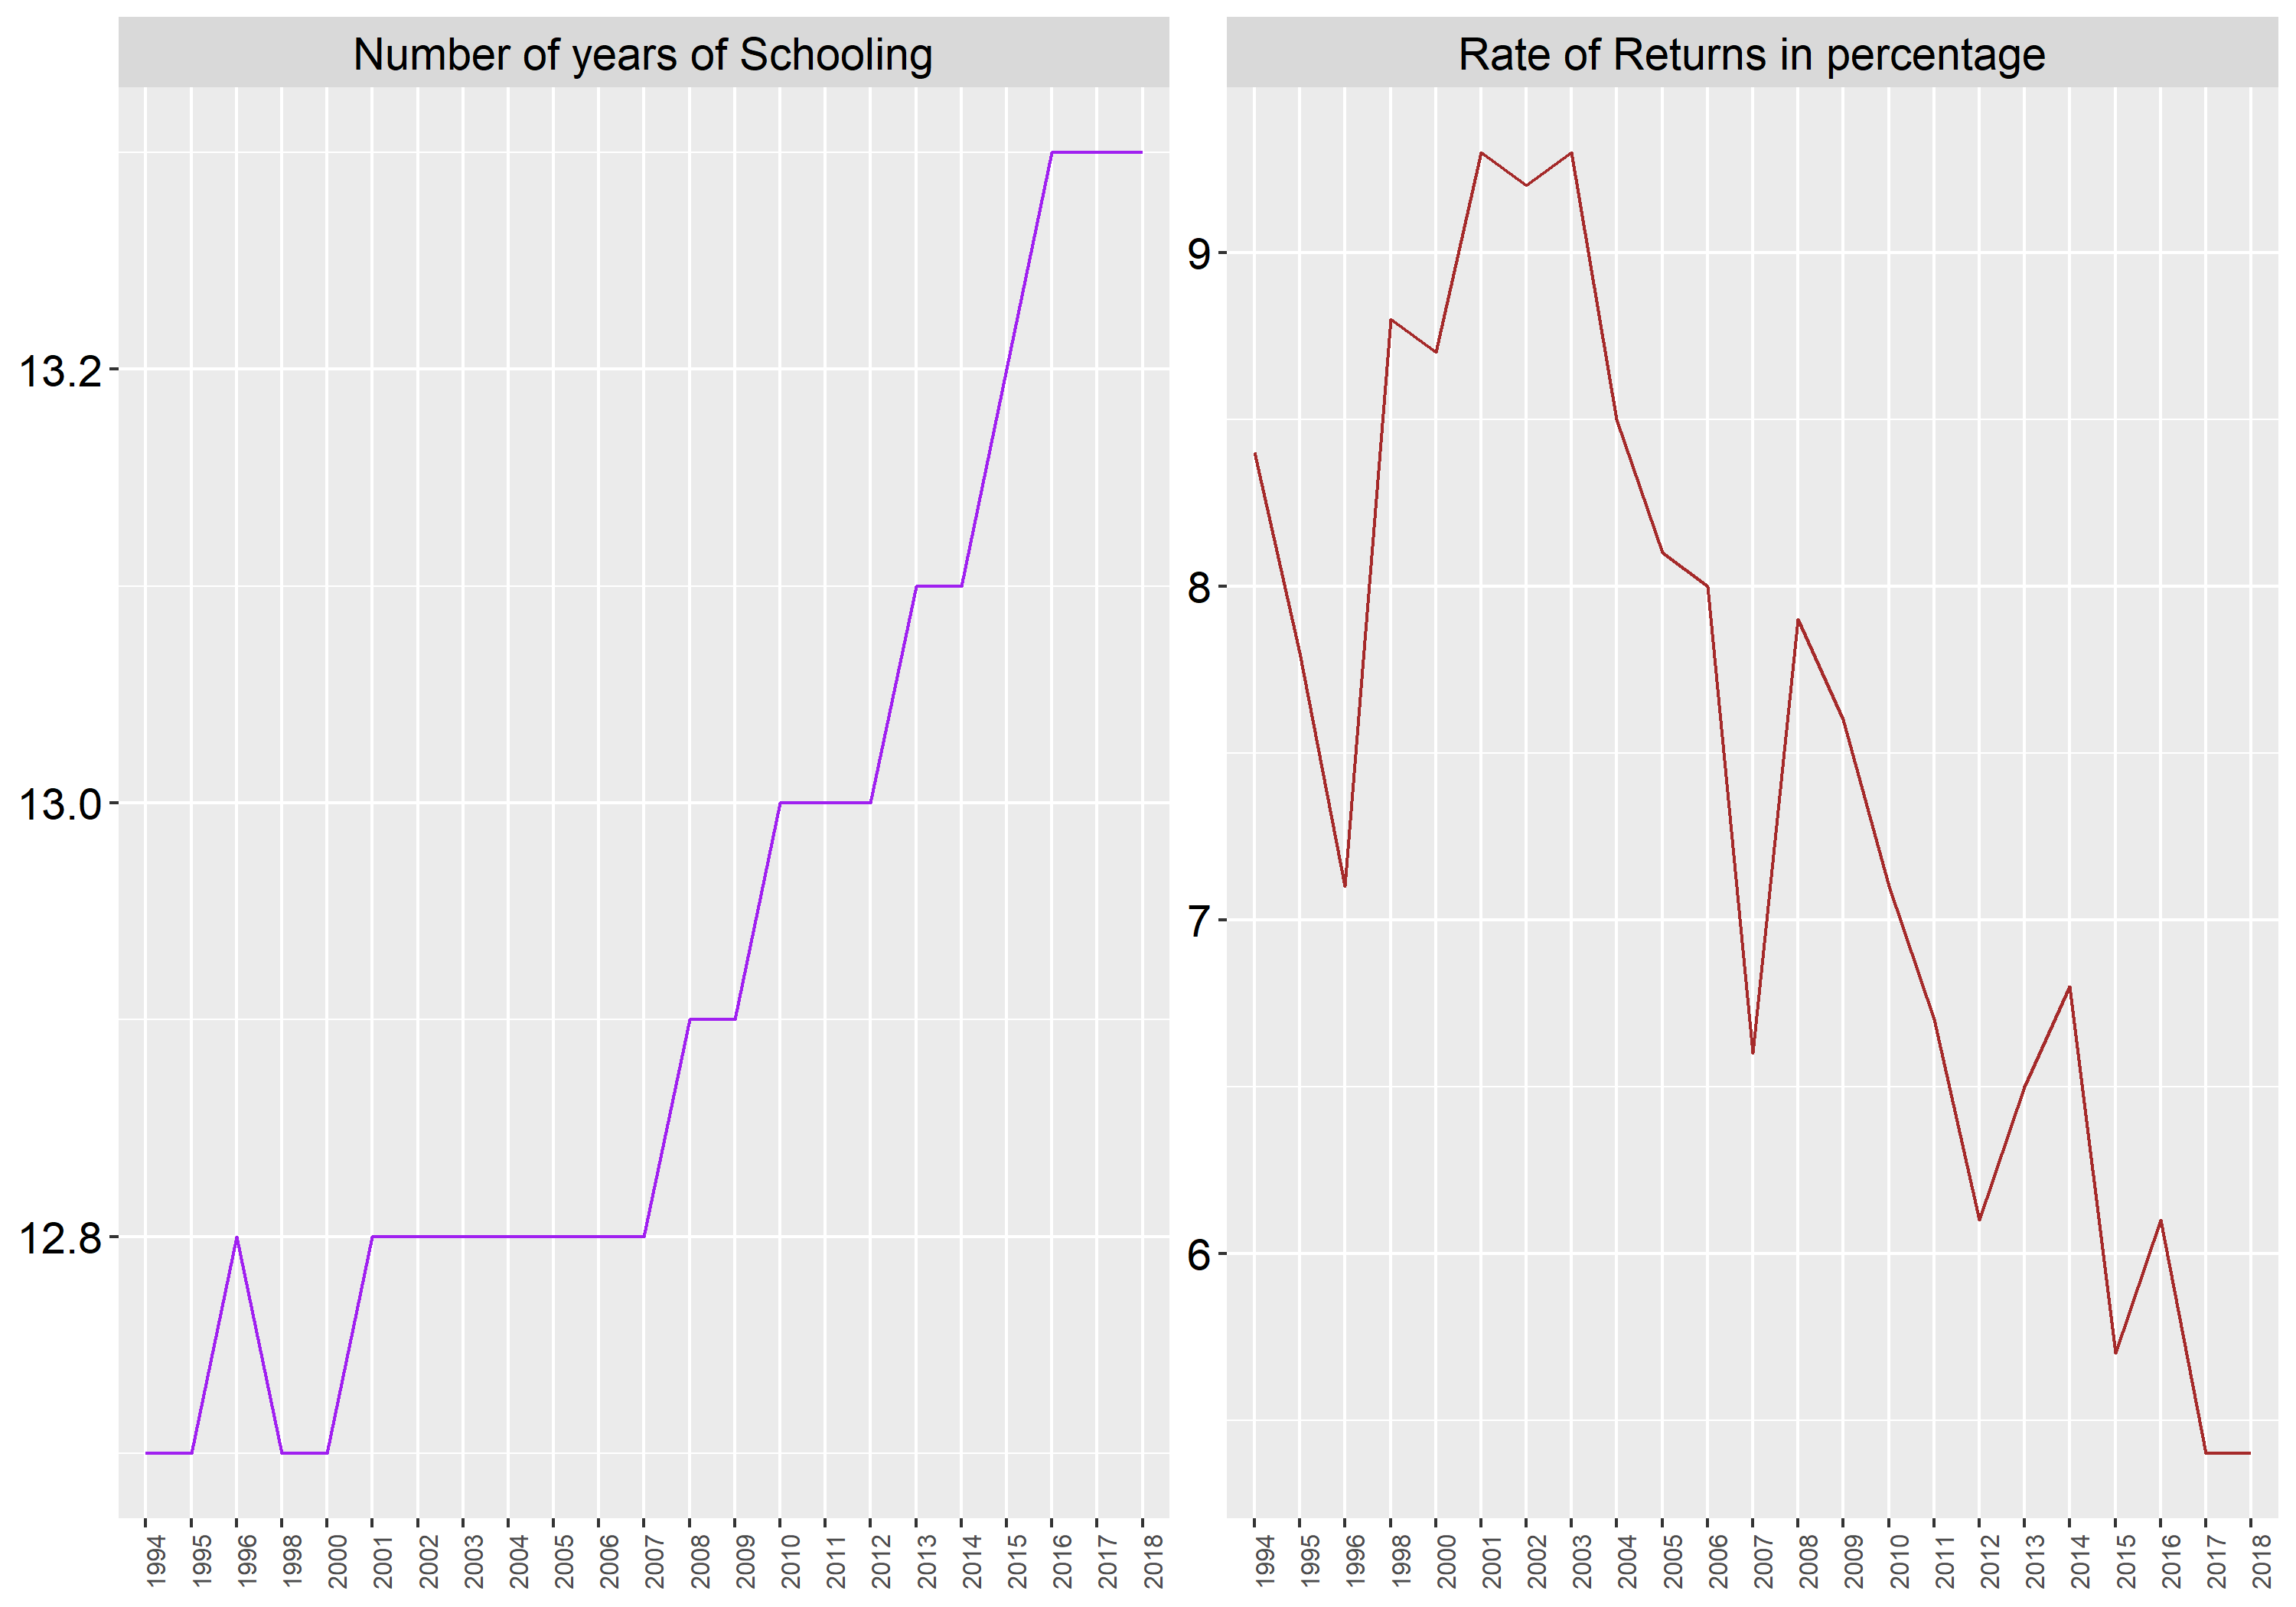
\includegraphics[width=5in]{hp_rs.png}
			% plot 1
		\end{minipage}
			\caption{Labor Force Distribution by Educational Level (Rosstat)}\label{fig:1.01a}
	\end{figure}
\end{center}


\vspace{-2em}
Figure \ref{fig:5.1} demonstrates earnings ratio by educational level (secondary education is equal to 100\%) for 1998, 2006, and 2018. The graph depicts a pronounced gap in the wages of people with secondary or vocational education compared to those with university level especially in earlier years in Russia.

% \vspace{-0.2in}
\begin{center}
	\begin{figure}[htbp!]
\begin{minipage}[b]{1\linewidth}
			\centering
		%	\hspace*{-0.6in}
			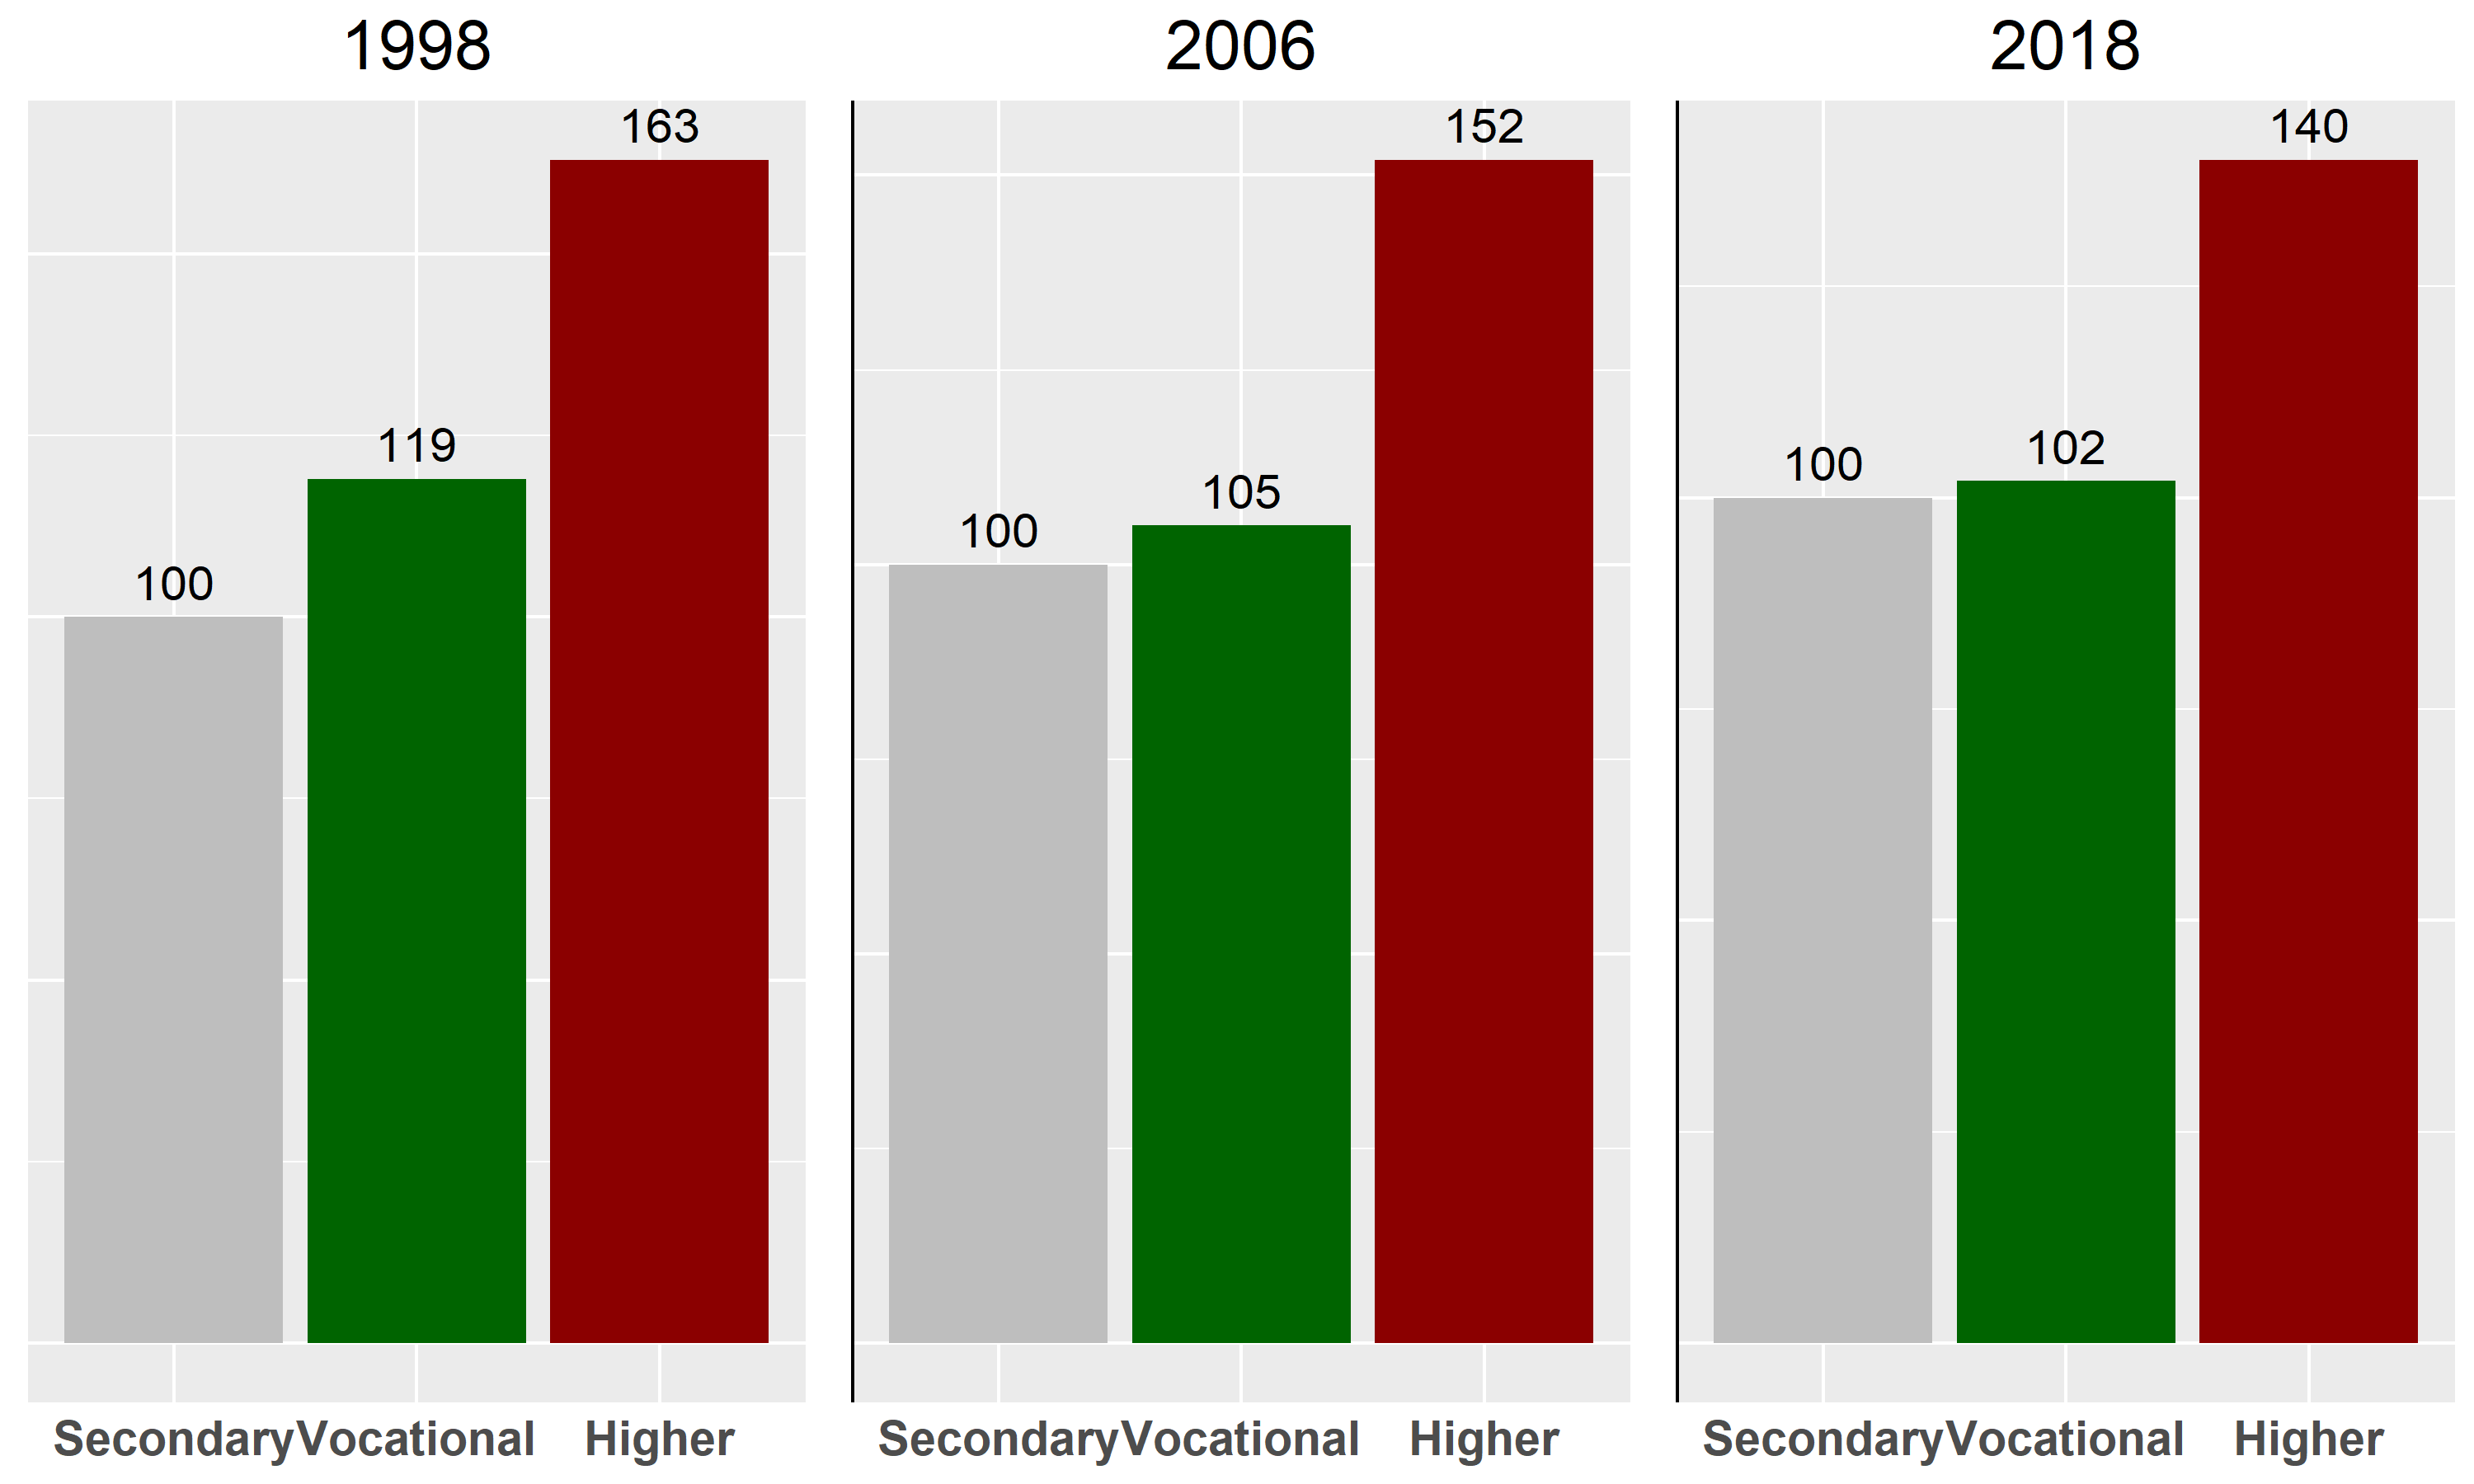
\includegraphics[width=6in]{earnings_ratio.png}
			% plot 1
		\end{minipage}
			\caption{Earnings Ratio by Educational Level (Secondary Education = 100\%)}\label{fig:5.1}
	\end{figure}
\end{center}

\vspace{-0.2in}

\begin{center}
	\begin{figure}[htbp!]
\begin{minipage}[b]{1\linewidth}
			\centering
			\hspace*{-0.3in}
			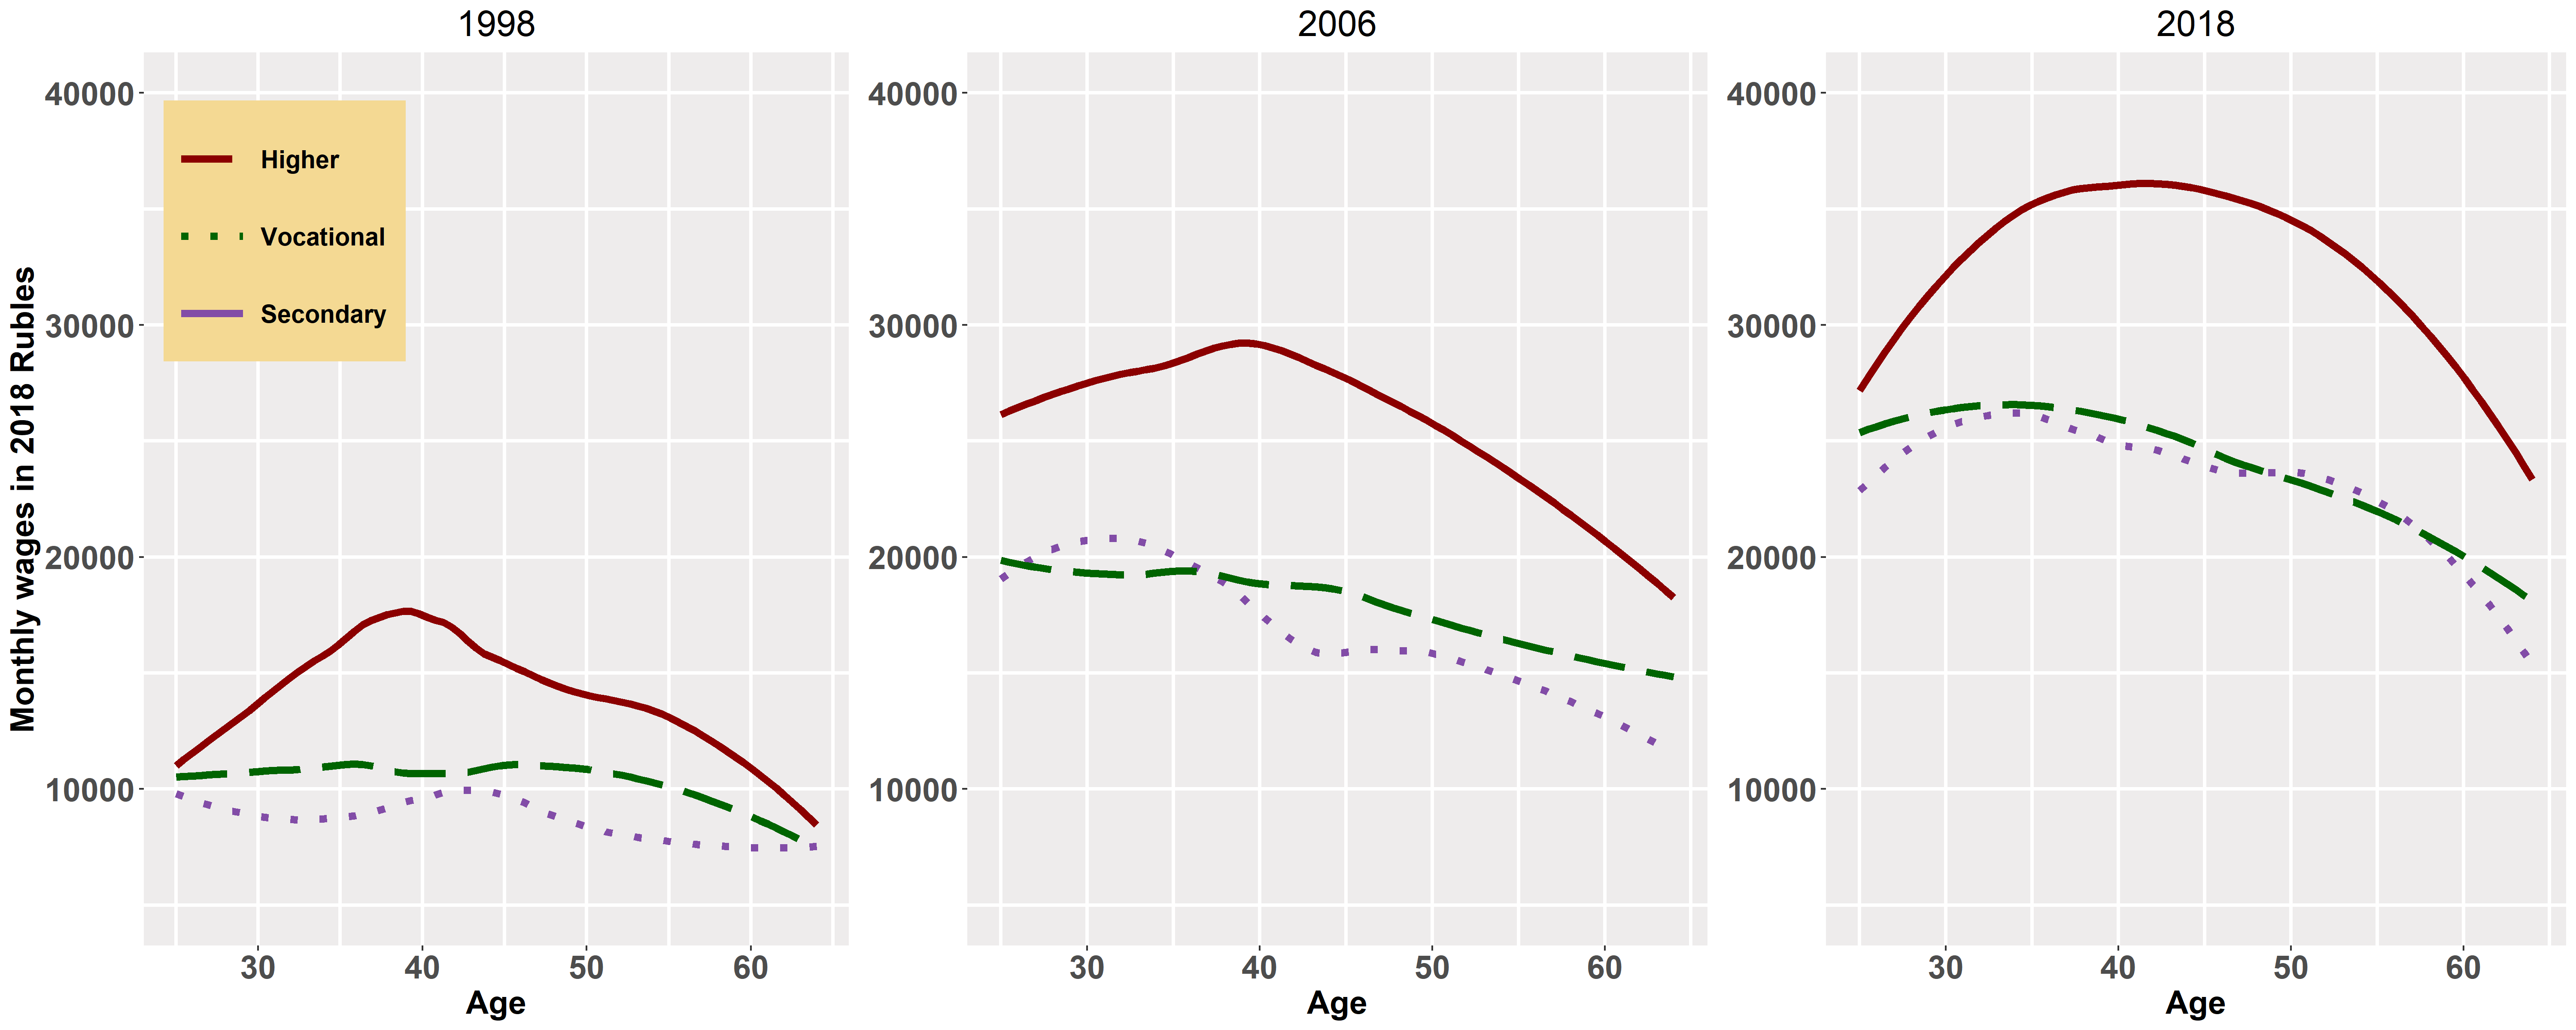
\includegraphics[width=6in]{earnings_by_level.png}
			% plot 1
		\end{minipage}
			\caption{Age-earning Profiles by Level of Education}\label{fig:5.2}
	\end{figure}
\end{center}

% \vspace{-0.2in}

Figure \ref{fig:5.2} displays age-earning profiles in Russia by education level. There is a clear concave pattern for higher level, whereas for secondary and vocational levels, the association between wages and age is almost flat or descending. While the gaps are declining between higher and secondary, they are increasing between higher and vocational. 

Figure \ref{fig:1.2} summarizes the results, showing rates of overall and gender-wise returns to education in Russia for the period 1994-2018: the percentage increment in a person's earnings due to one additional year of schooling. Overall, one can notice a moderate curved growth in returns to education in Russia, achieving its peak in the early 2000s (returns of 9.8\%), which is followed by a downward pattern (returns of 5.6\% by 2018). The values of returns to schooling in recent years in Russia seem to lag far behind the global average of 9.5\% \parencite{Psacharopoulos_Patrinos2018}. Education payoffs for women are higher than those of men, but the difference appears to have narrowed in recent years.

Figure \ref{fig:1.3}, panel (a) displays rates of returns to Higher and 
Vocational education (as compared to Secondary education) in Russia for the 
period 1994-2018. The results suggest that on average wage premiums to 
university education in Russia are roughly 3-5 times greater than to 
vocational schooling. The observed trend for premiums to both Vocational 
and Higher education levels is similar to the trend for education in 
general with the following peaks: 18\% per year for Higher education and 
6\% per year for Vocational education compared to the average earnings of 
workers with a Secondary education. The interesting pattern to note from 
panel \ref{fig:1.3a} is the apparent co-movement of vocational education 
and higher education - the higher education smoothing curve turns a bit 
more sharply than the one for vocational education, but their movement is 
matching, even at second-order levels of smoothness. Further, even though 
higher education premium remains much above the premium for vocational 
education, there is a perceptible narrowing of the difference in recent 
years. Panel \ref{fig:1.3b}, which is drawn from \cite{Telezhkina2019}, 
shows the interesting pattern of higher education enrollment rates for the 
population of 17-25 year olds . Panel \ref{fig:1.3b} shows the downturn in 
returns reflected in enrollments, with the peak in enrollments coming about 
10 years later. The latest estimate of the returns to higher education in 
the Russian Federation is about 8\%, which is just below the EU average of 
about 10\% and the global average of 15\% 
\parencite{Psacharopoulos_Patrinos2018}, and declining, in line with the 
expansion that took place up to 2009. 

\begin{figure}[htbp!]
\caption{\textbf{Rates of Returns to Higher and Vocational Education in Russia, RLMS 1994-2018}}\label{fig:1.3}
         \centering
         \begin{subfigure}[b]{0.5\textwidth}
                 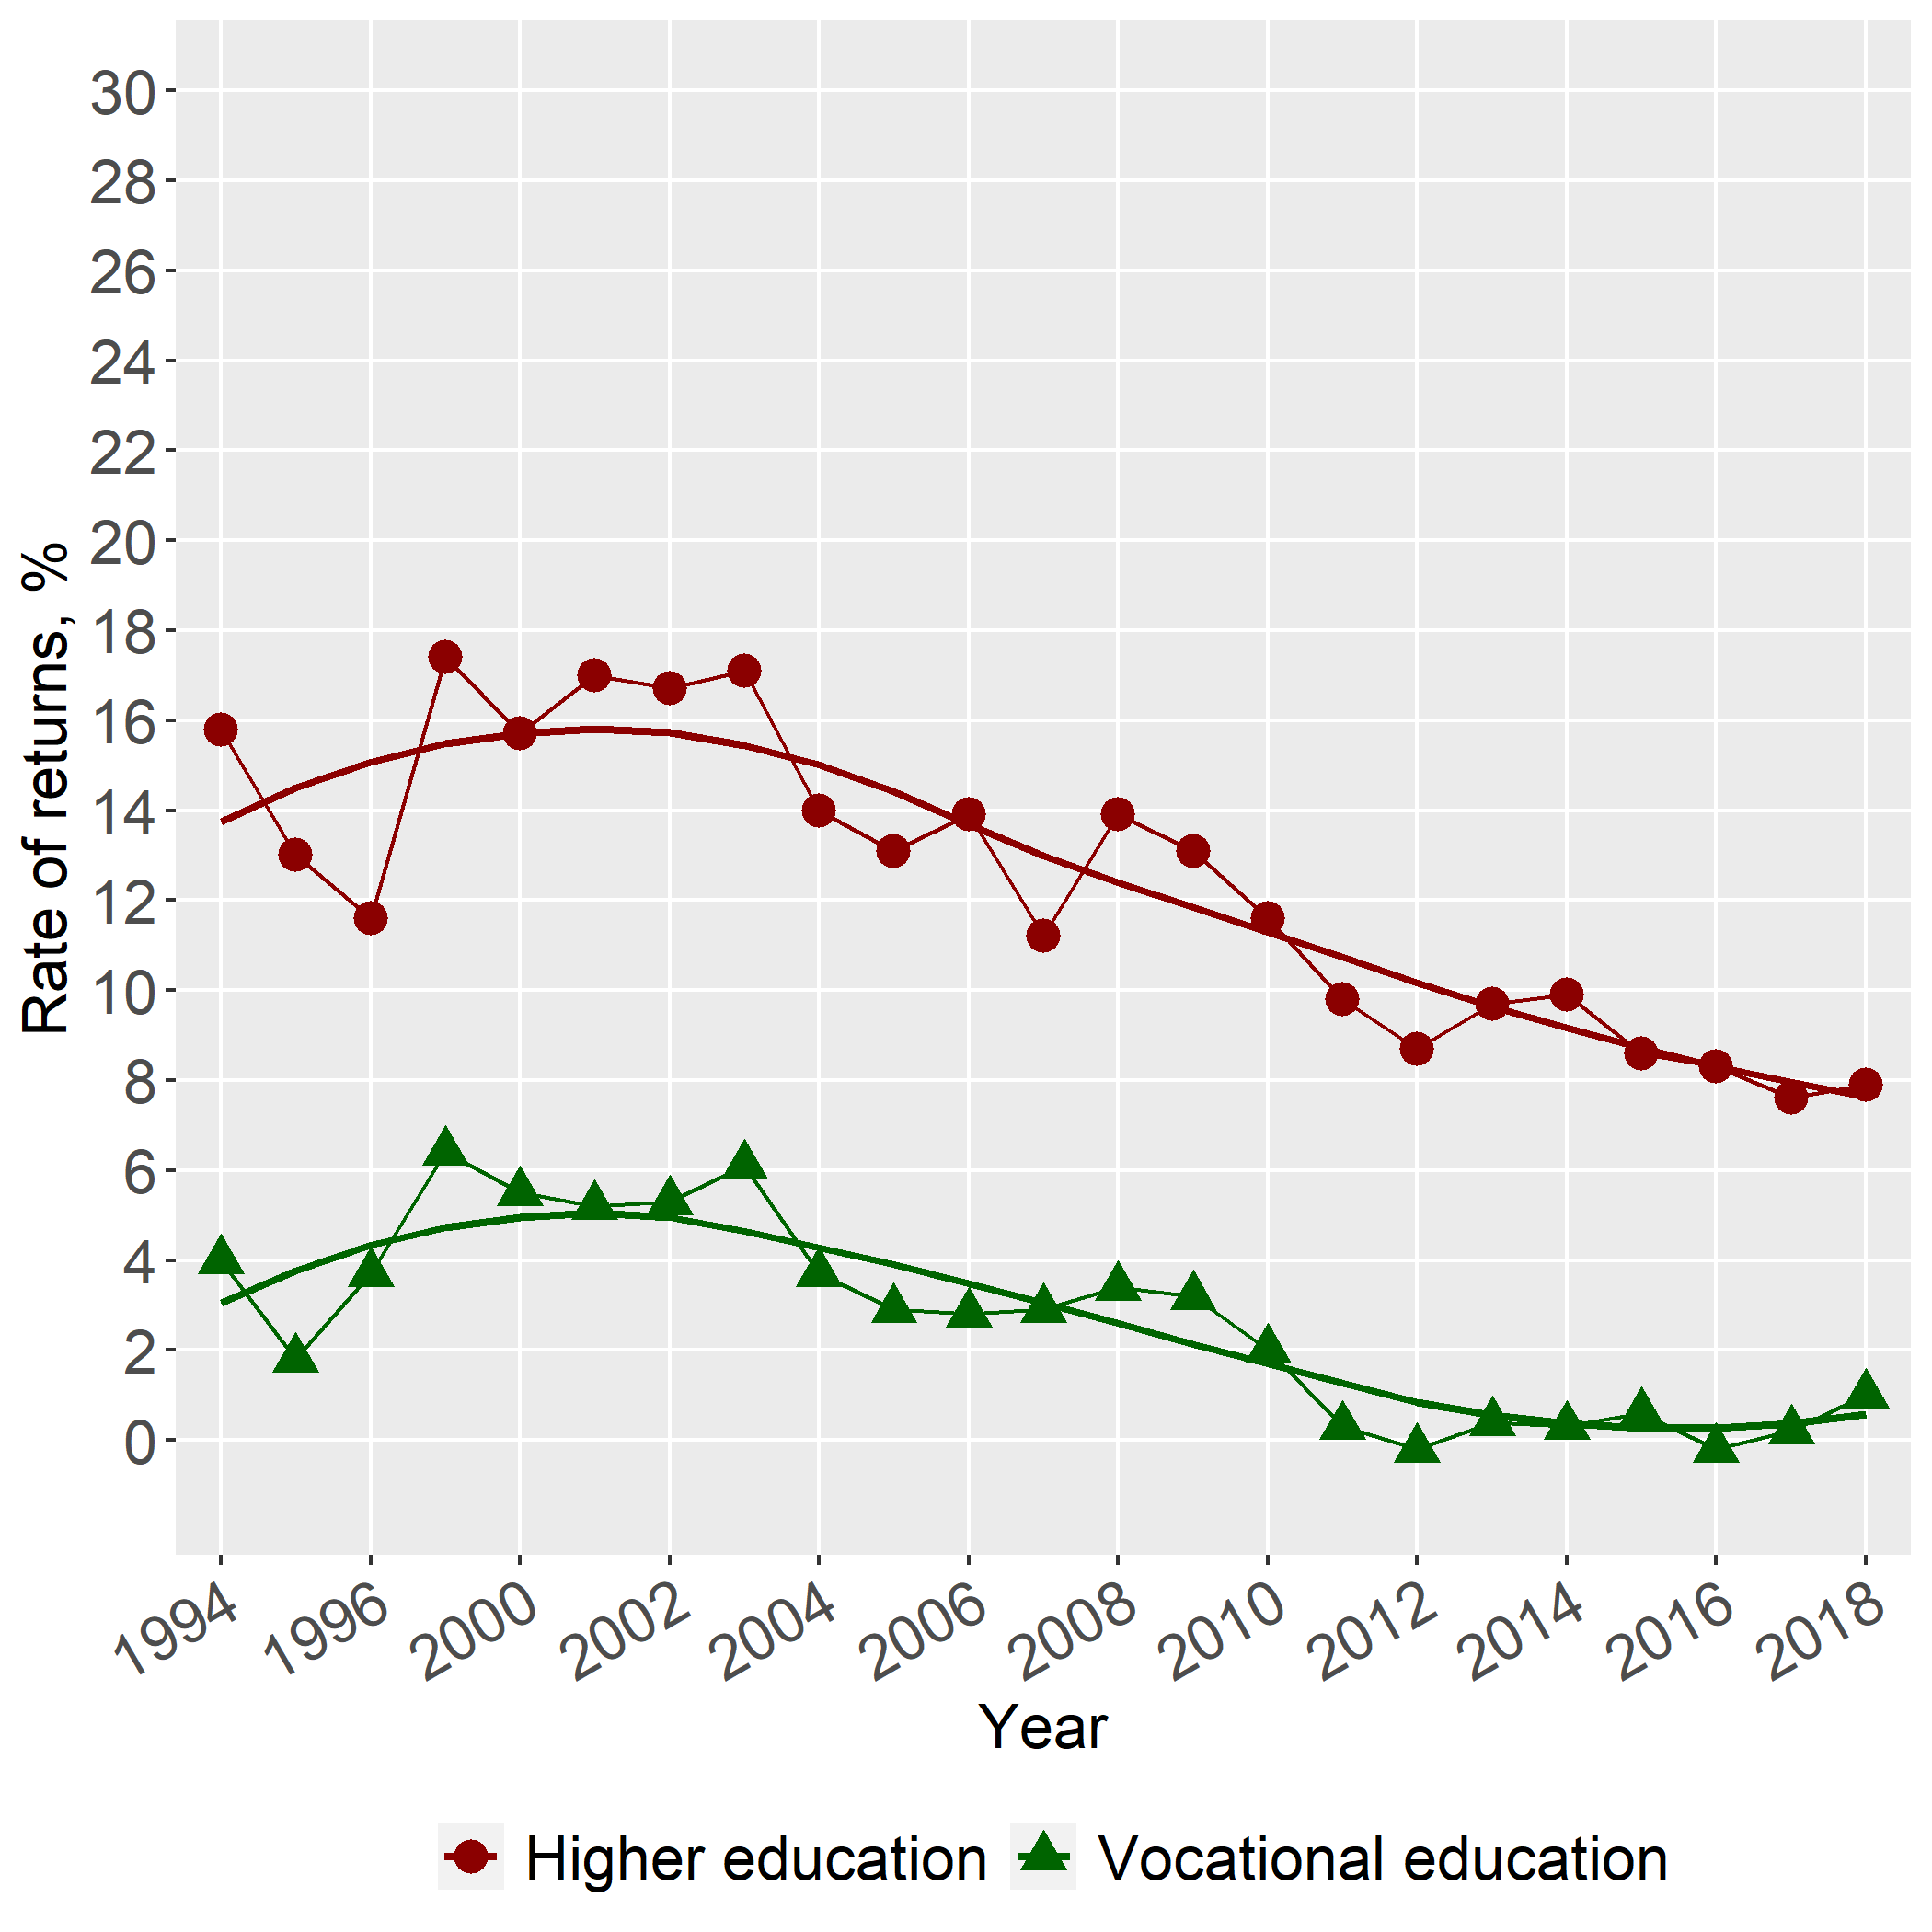
\includegraphics[width=\textwidth]{re_HE_all.png}
                 \caption{Rates of Return}
                 \label{fig:1.3a}
         \end{subfigure}%
         ~ %add desired spacing between images, e. g. ~, \quad, \qquad, \hfill etc.
           %(or a blank line to force the subfigure onto a new line)
         \begin{subfigure}[b]{0.5\textwidth}
                 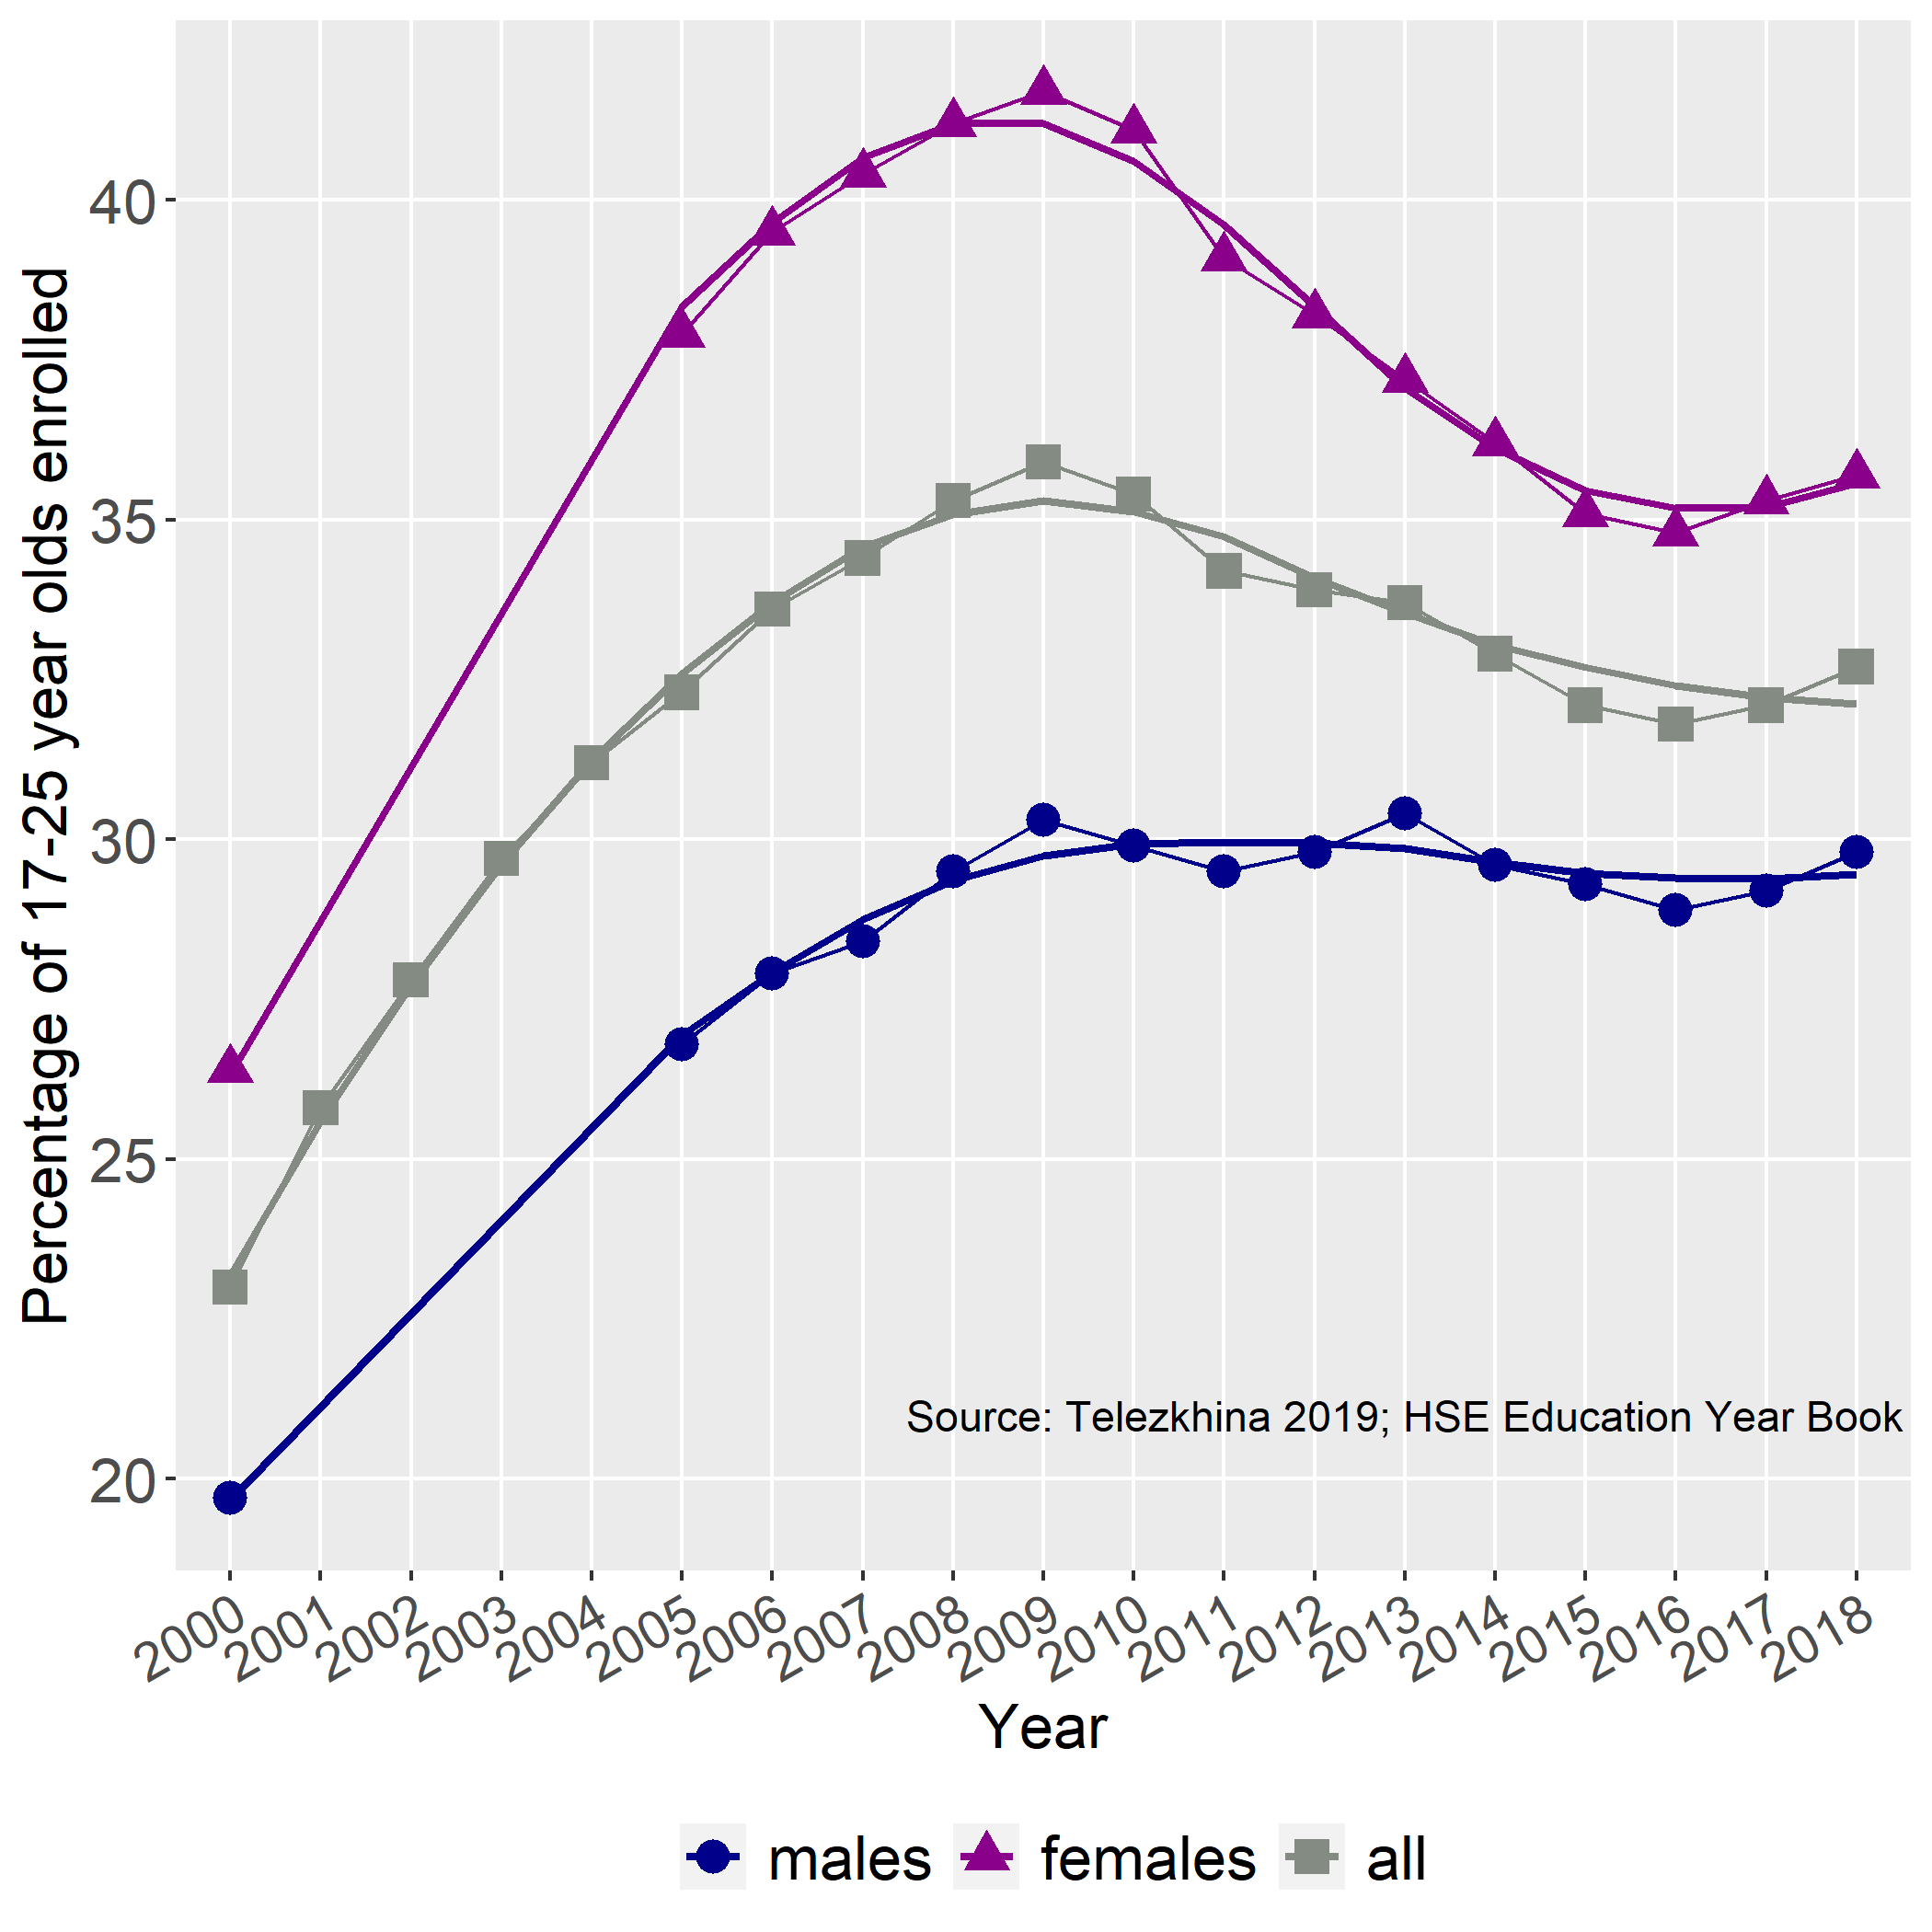
\includegraphics[width=\textwidth]{telez1a.png}
                 \caption{Enrollment in Higher Education}
                 \label{fig:1.3b}
         \end{subfigure}
     \end{figure}


\begin{figure}[htbp!]
 \centering
 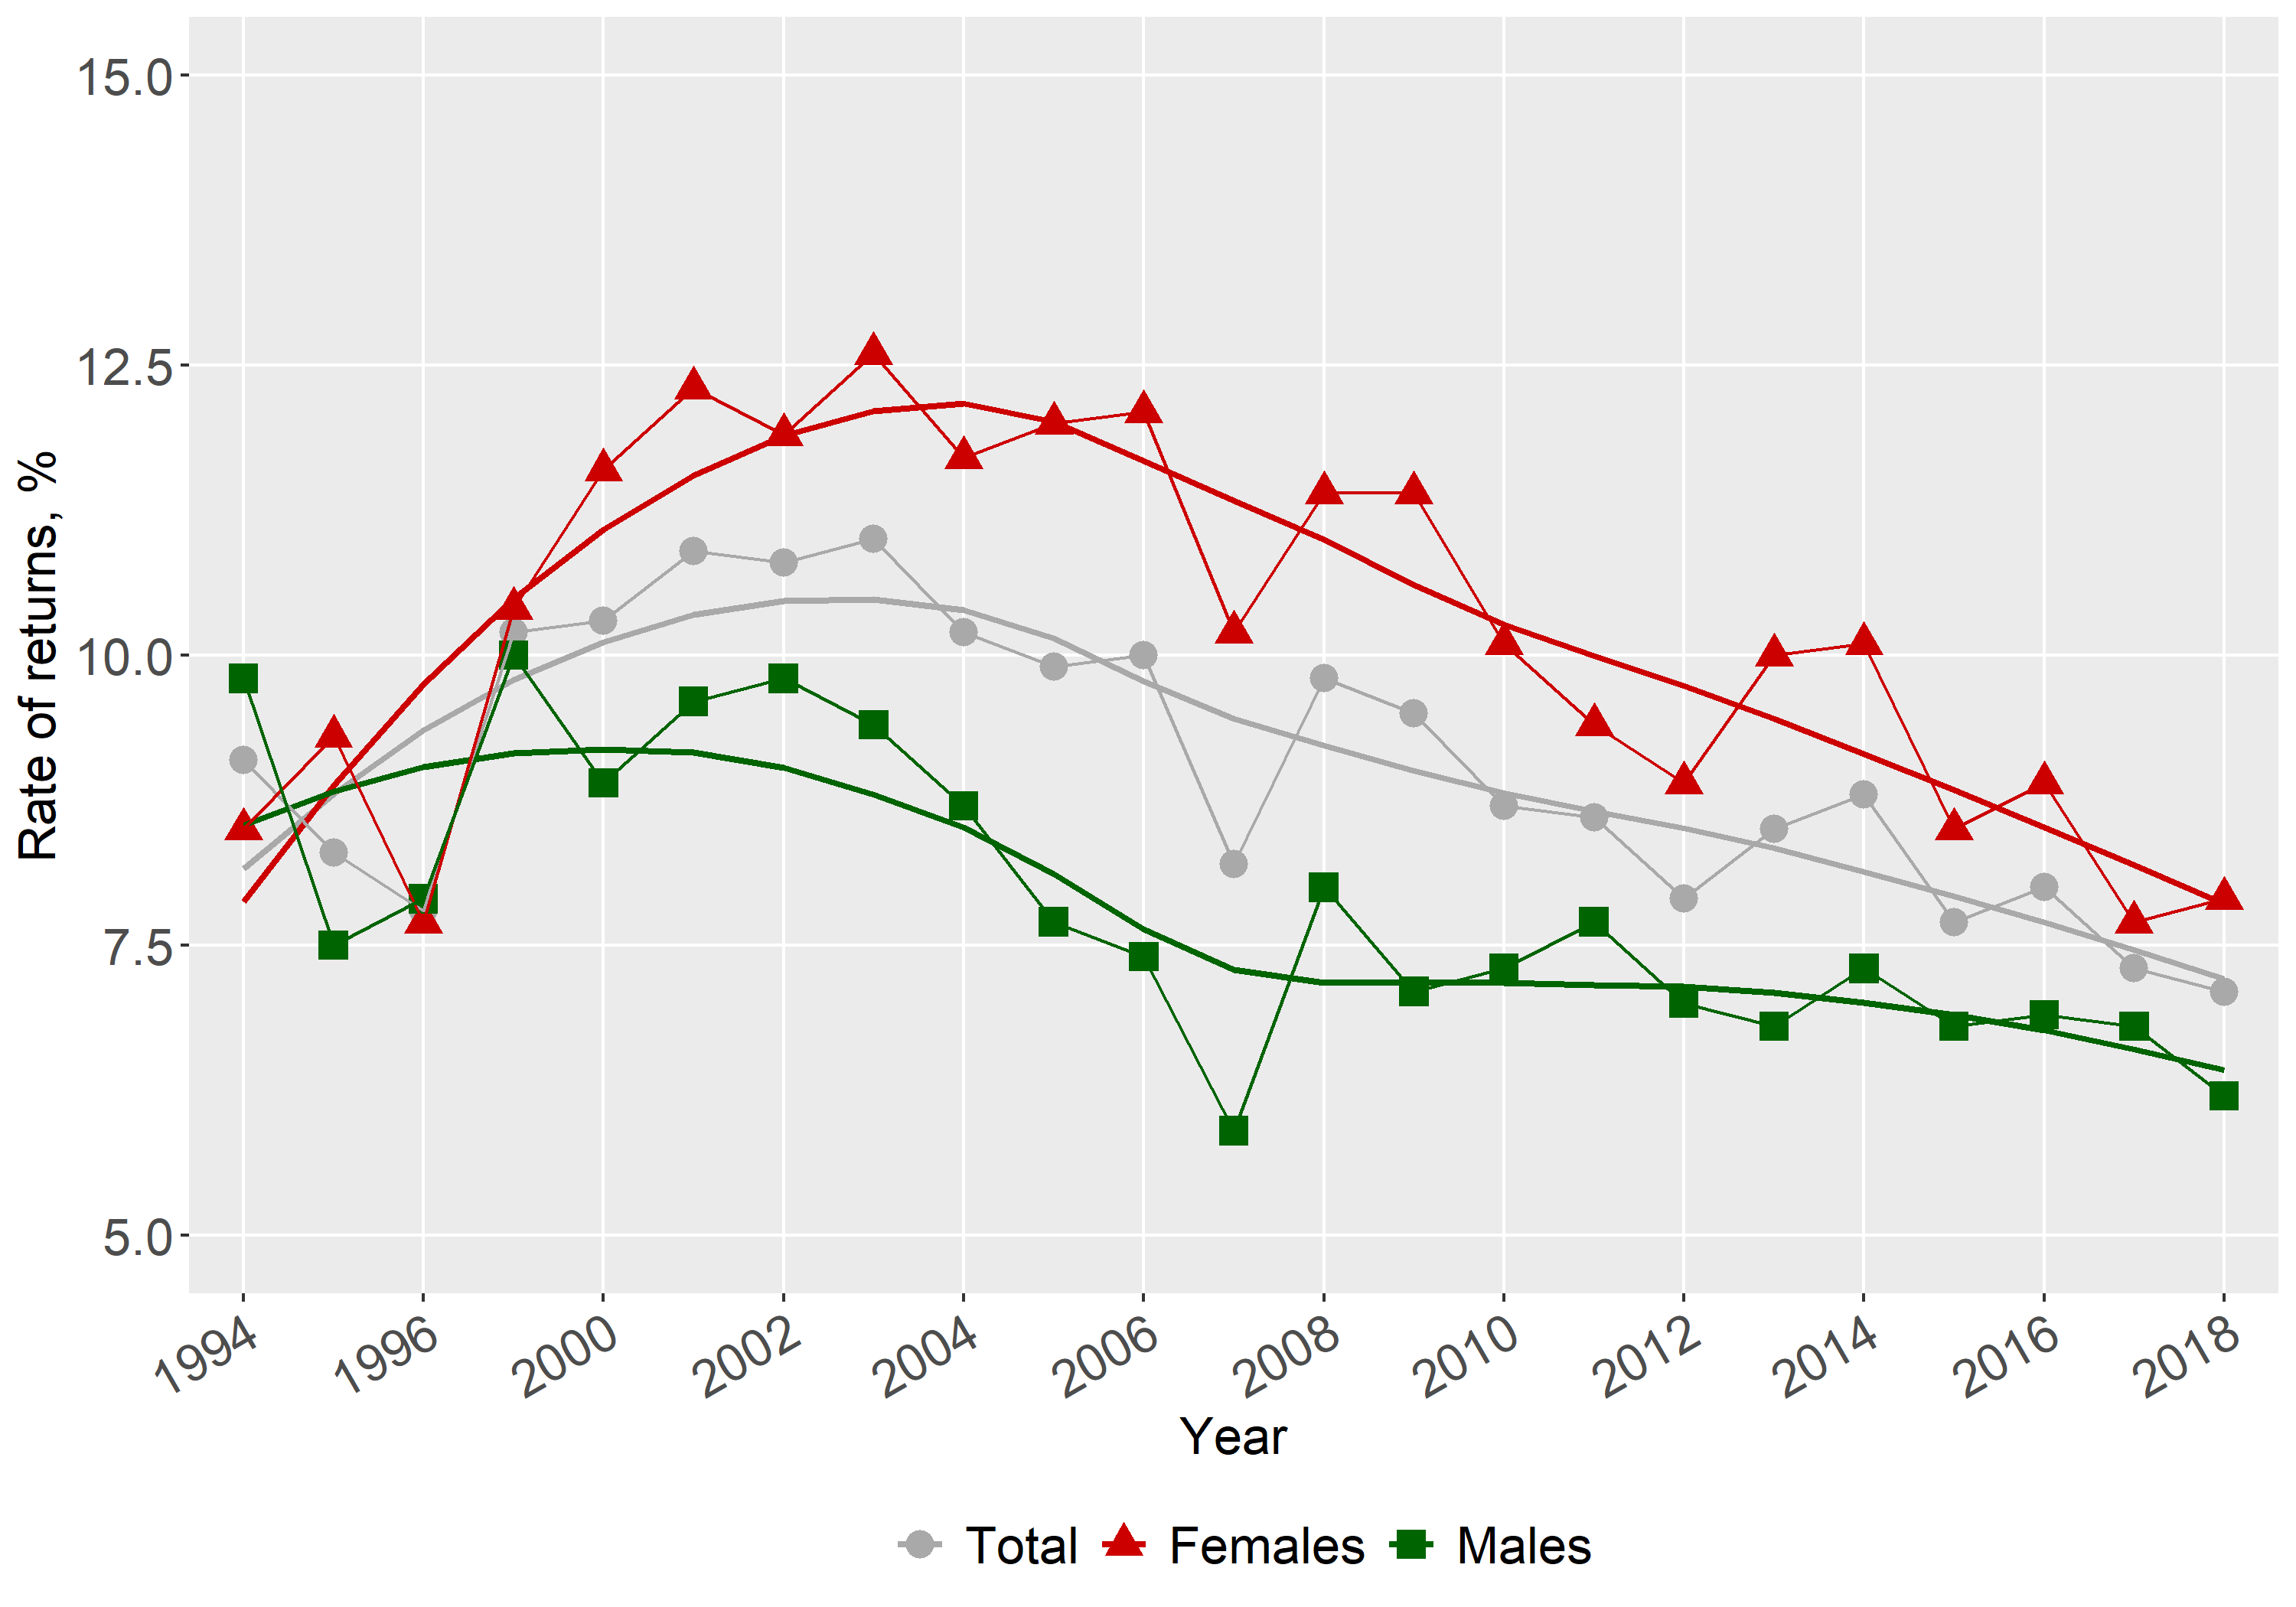
\includegraphics[width=\textwidth, height=275pt]{re_edu.png}
 \caption{Rates of Returns to Education in Russia, RLMS 1994-2018}\label{fig:1.2}
\end{figure}

\begin{figure}[htbp!]
  \begin{minipage}[b]{.5\linewidth}
     \centering
     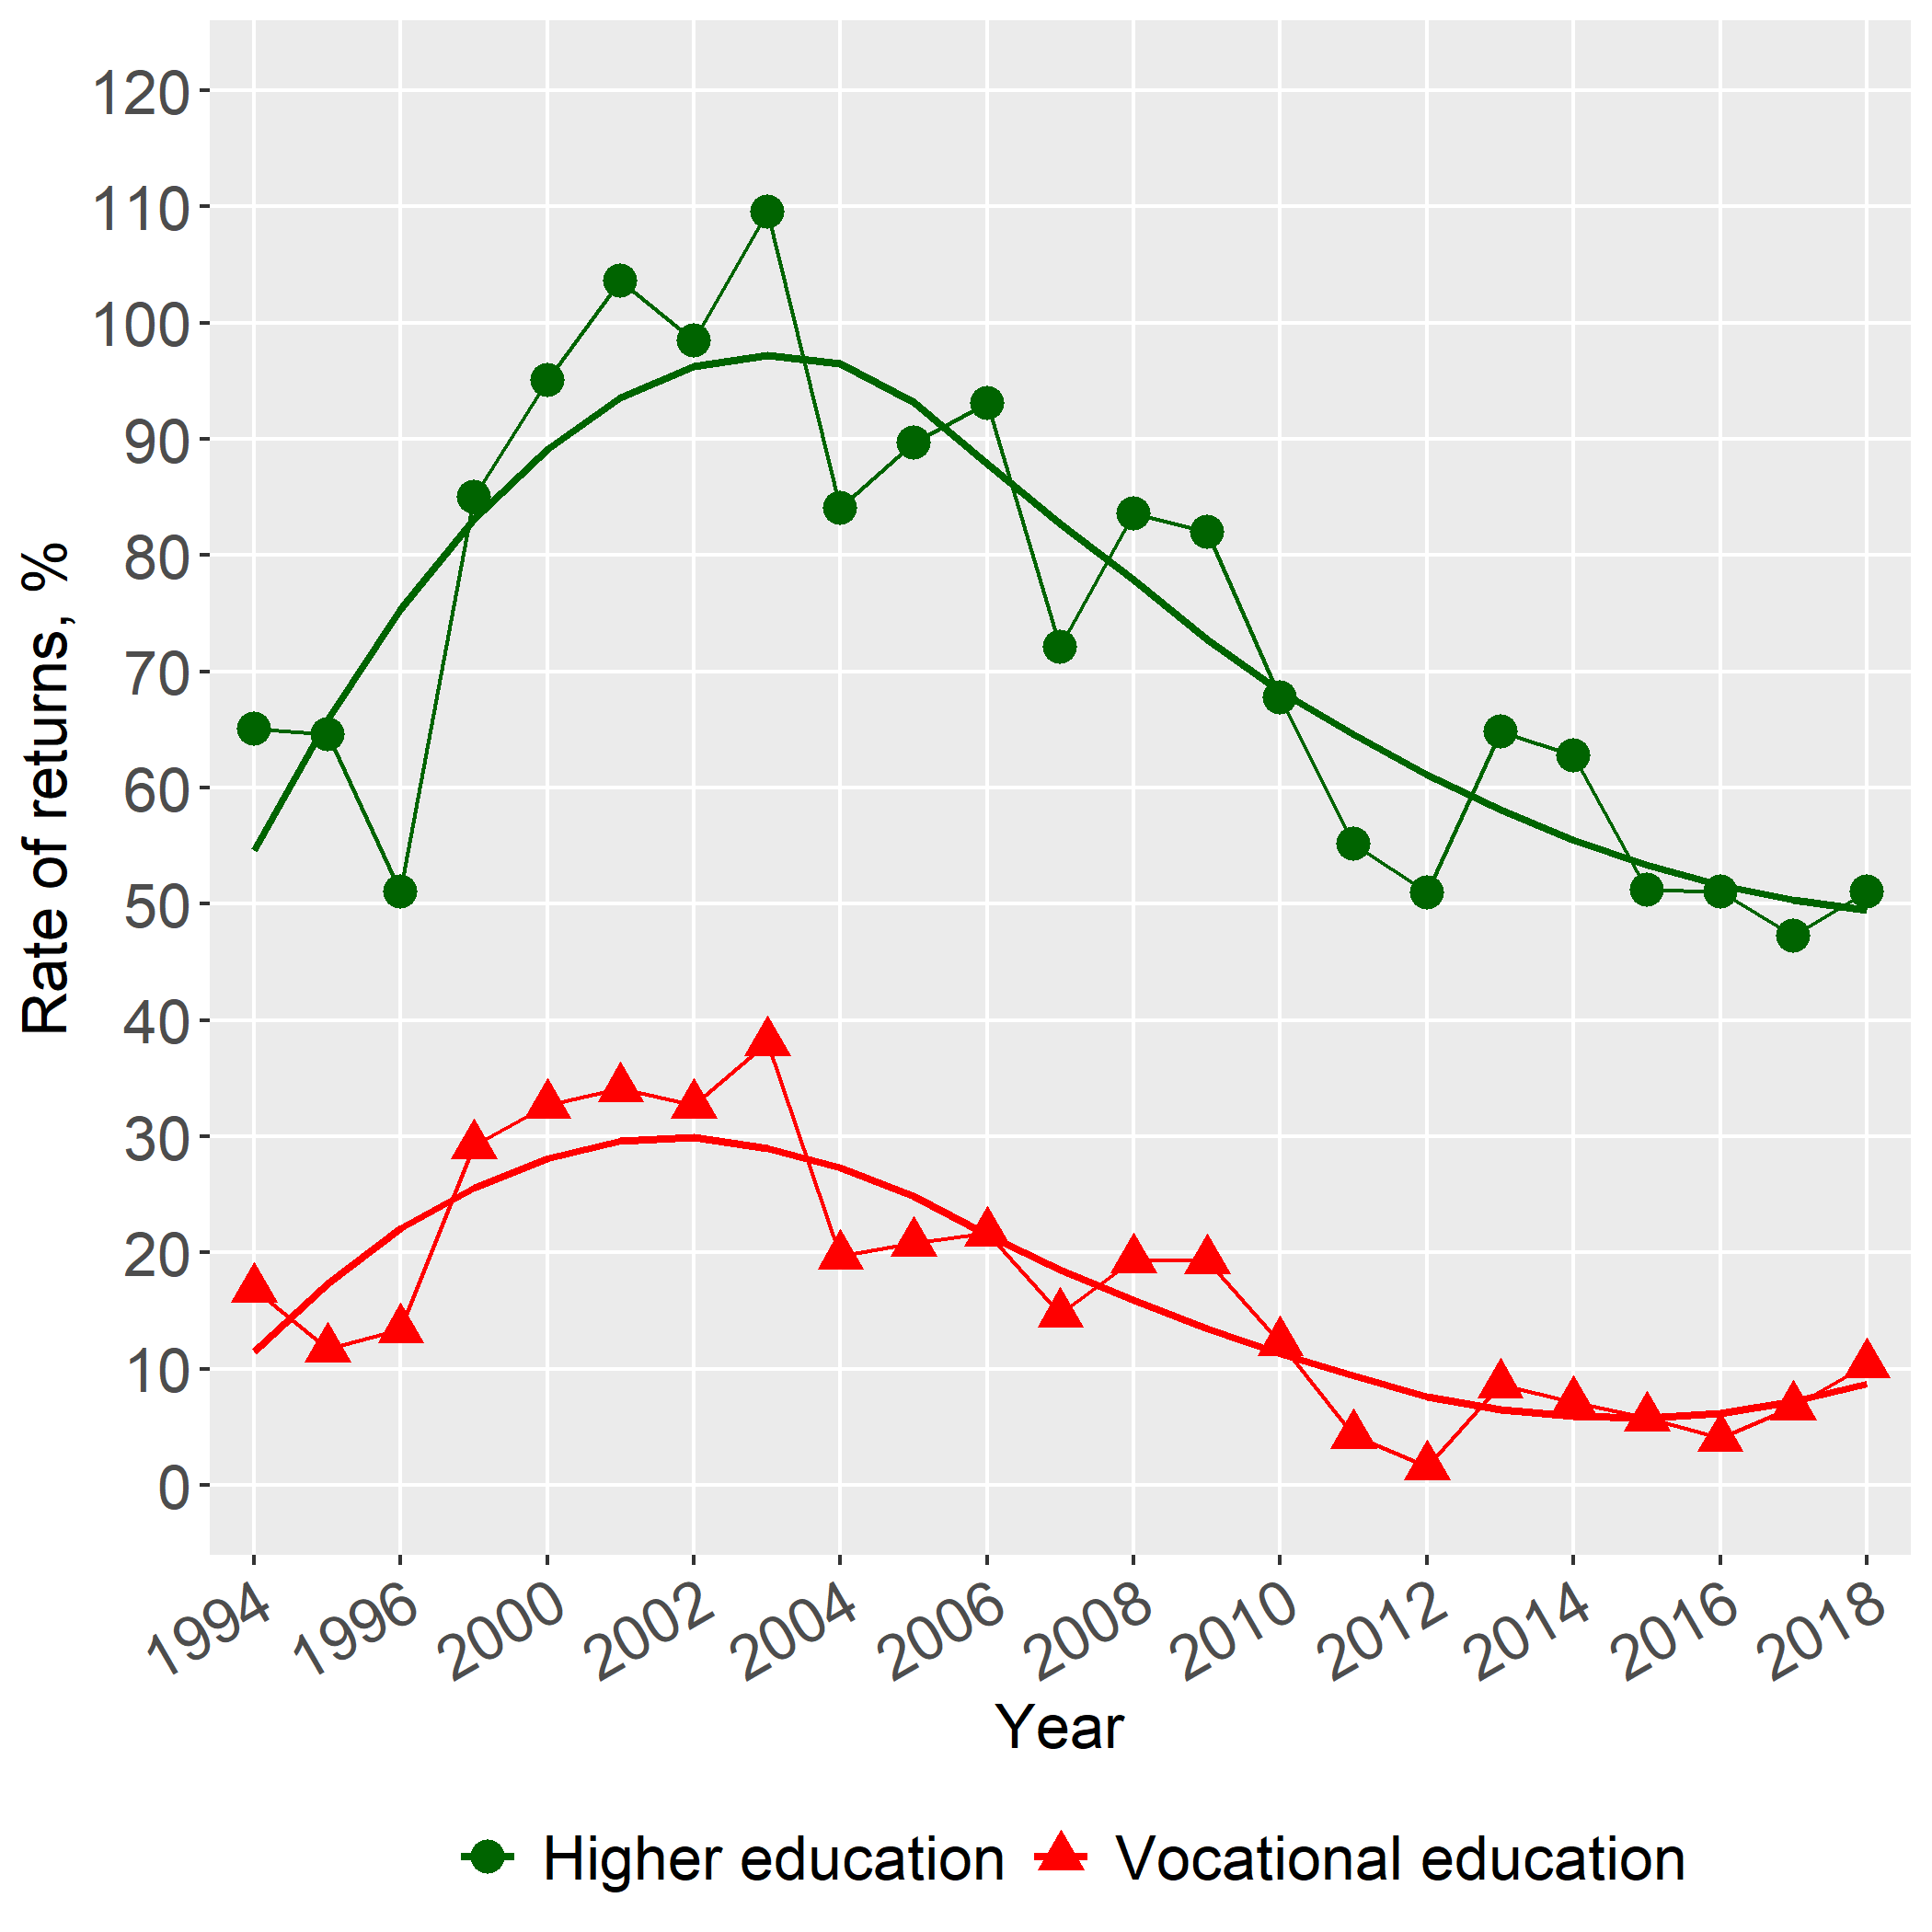
\includegraphics[width=\textwidth]{re_HE_f.png}
     % plot 1
     \subcaption{Females}\label{fig:1.4a}
  \end{minipage}
  \hfill
  \begin{minipage}[b]{.5\linewidth}
     \centering
     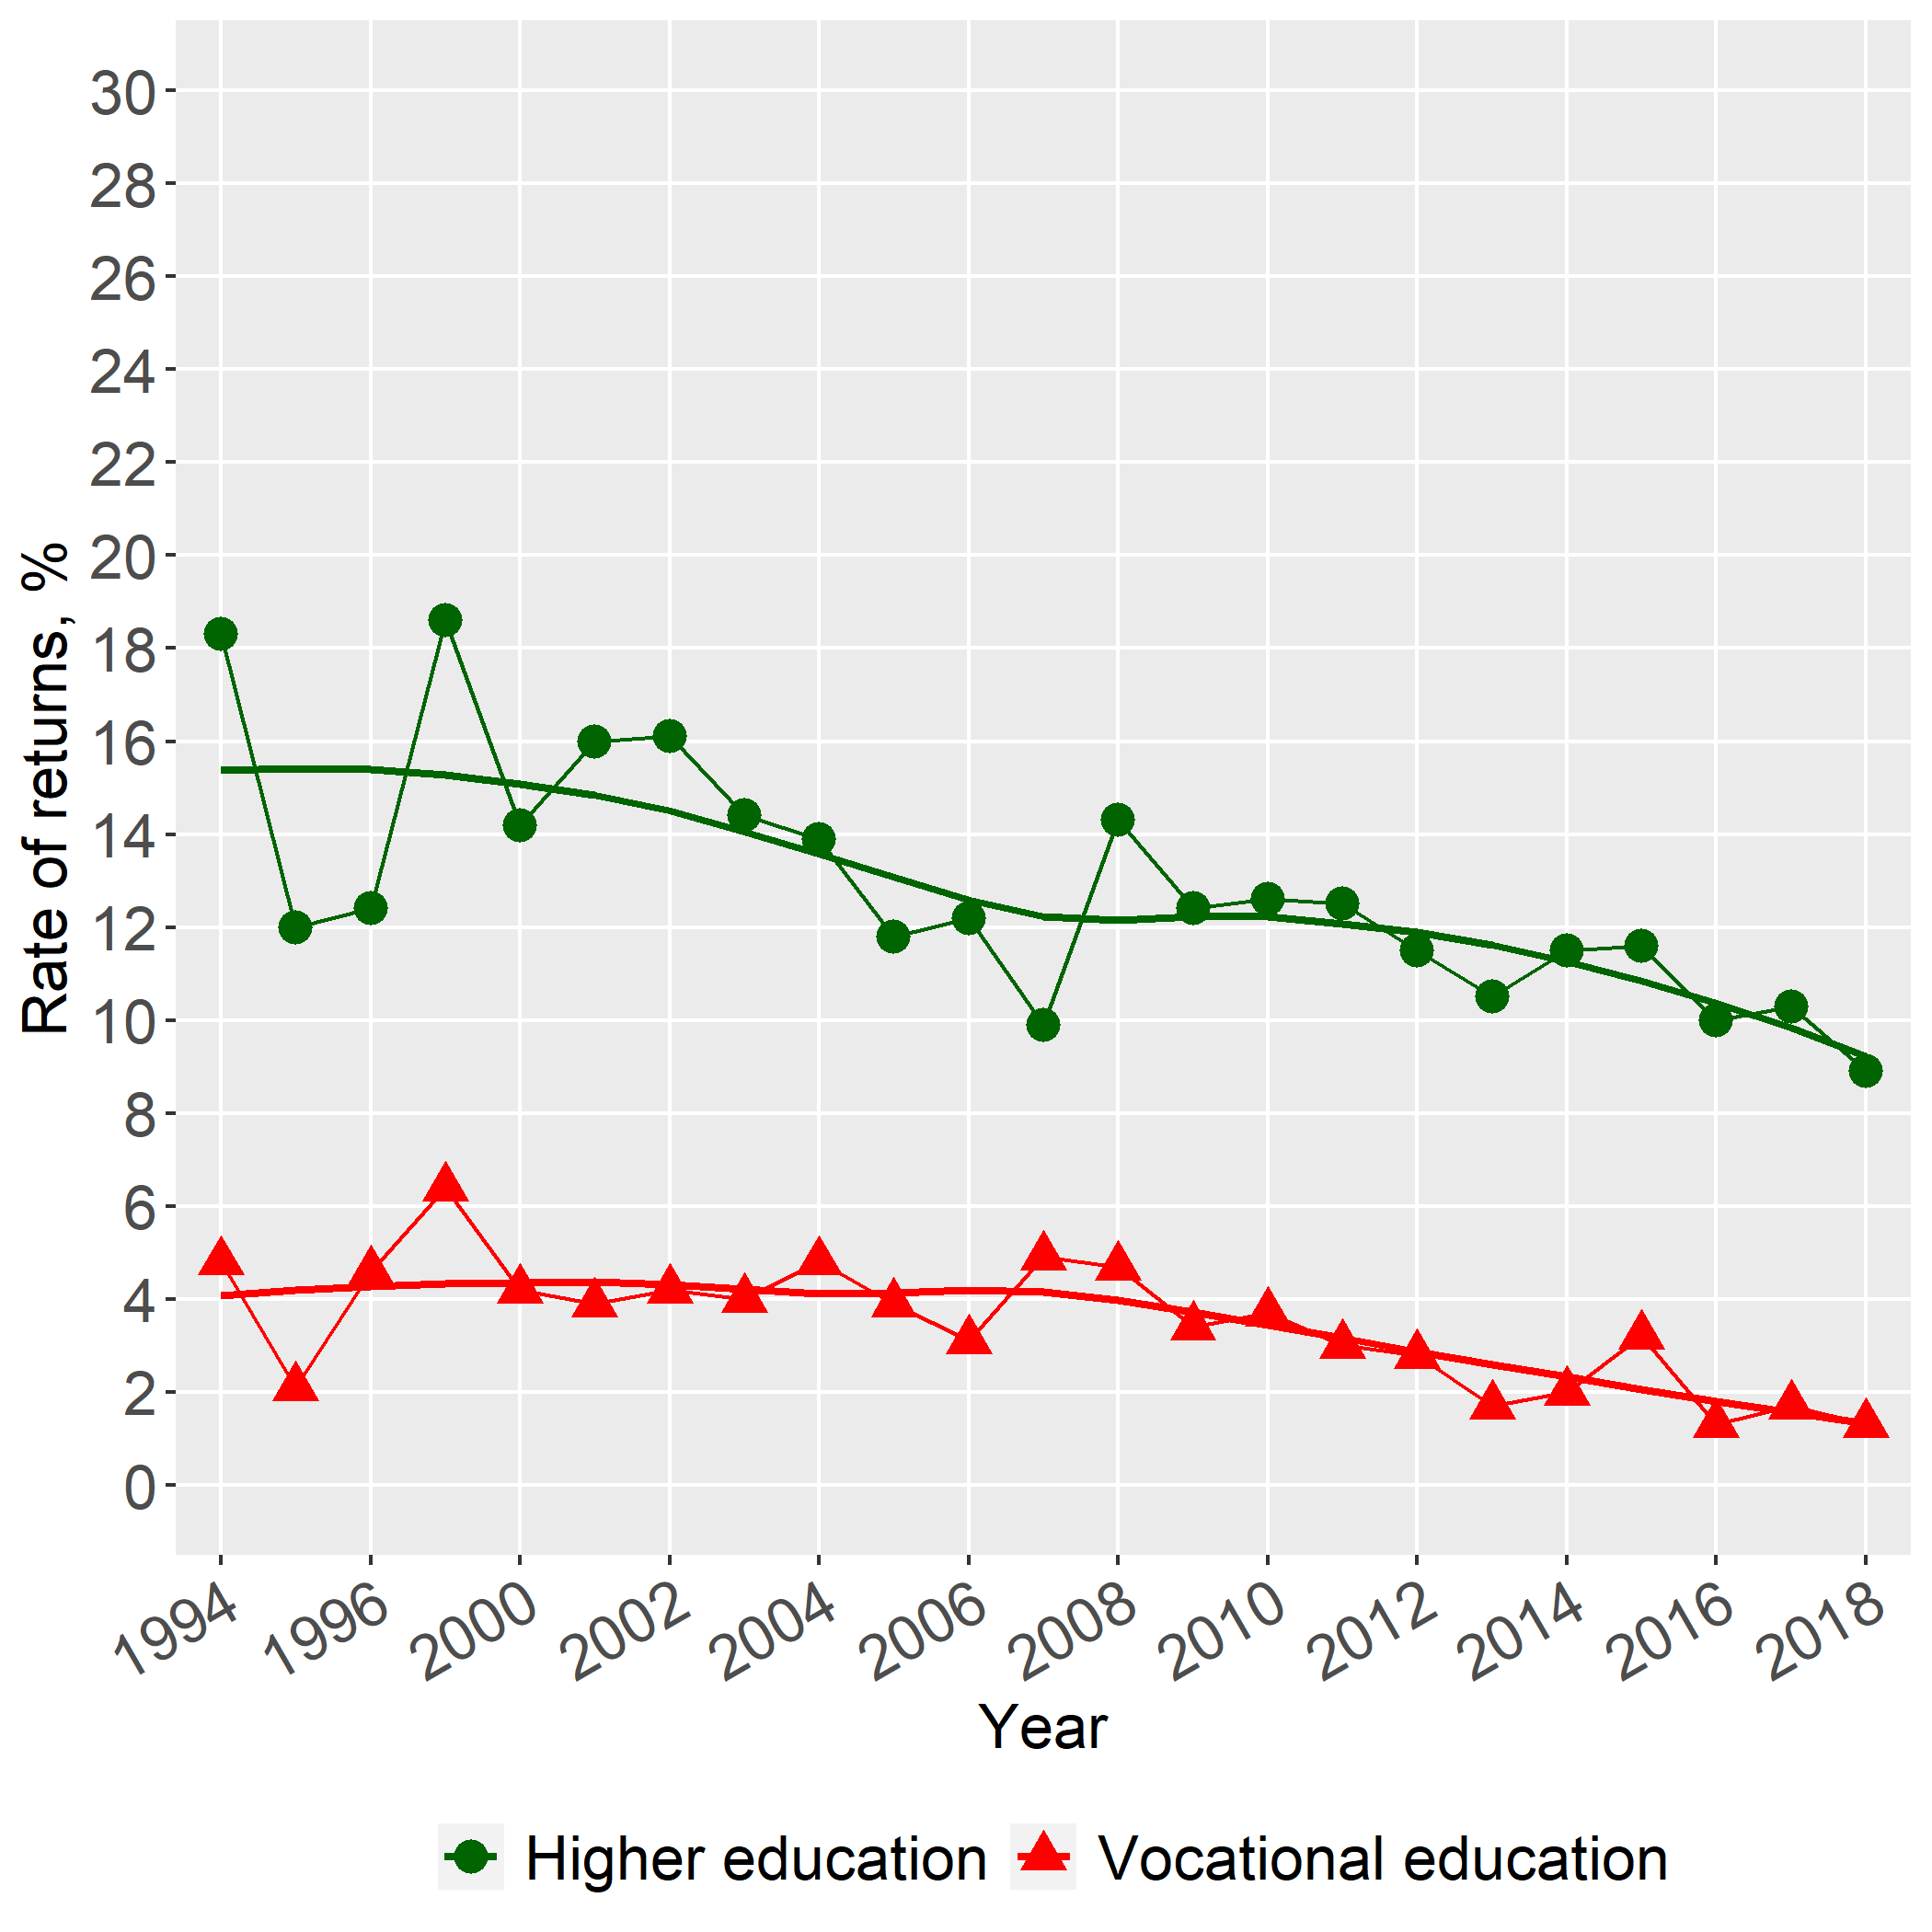
\includegraphics[width=\textwidth]{re_HE_m.png}
     % plot 2
     \subcaption{Males}\label{fig:1.4b}
  \end{minipage}
  \caption{Rates of Returns to Higher and Vocational Education in Russia, RLMS 1994-2018}\label{fig:1.4}
\end{figure}

When estimated separately by gender, we find trend variation by gender. The results from estimation of earnings functions show that annual returns to Higher education for males varied from 9\% to 15\%, whereas women's returns are described by an inversely U-shaped pattern, reaching their maximum of 28\% in 2003. Within roughly the last 5 years, wage premiums to higher education for women have stabilized at around 12\%, a couple of percentage points ahead of men.  Gender wise enrollment rates in higher education (not shown) ten years later appears to match the differences in rates of return, strengthening the hypothesis that market rates of return to education in Russia do indeed influence individual continuing school decisions. 

A similar comparative picture is observed with respect to vocational education, albeit with a different kind of variation by gender (see Figure \ref{fig:1.4}): returns for males are almost flat within the time period while returns for females shows a concave pattern. The overall outcome concerning payoffs to schooling isolated by gender has been confirmed in a similar fashion by past studies \parencite[e.g.,][]{Cheidvasser2007}.

\section{Instrumental Variable Specification}

A strand of the literature holds that returns estimated from Ordinary Least 
Squares (OLS)  may be understated due to the possible presence of an 
omitted variable bias and resulting heterogeneity in the net benefits of 
additional schooling across individuals 
\parencite[e.g.,][]{Sakellariou2004, Akhmedjonov2011}. Instrumental 
variable (IV) regression is a method used to deal with these issues 
\parencite[e.g.,][]{Angrist1991, Card2001}.

In this study, we use indicators of the Parental Socio-Economic Status 
(SES) of individuals when the individuals were 15 year olds, as 
instrumental variables. Even though some authors think that family 
background related variables may suffer the same problem as an endogenous 
education variable, variables such as Father's education have been used 
instruments in earnings functions \parencite[e.g.,][]{Trostel2002, 
Sakellariou2004, Parker2006, Hoogerheide2012}. The reasoning is that 
variables such as parental education are related to the schooling level of 
an individual through genetic or environmental effects when an individual 
is a dependent child in a parent's household. However, parental variable 
direct influence on \textit{adult} earnings, independent of the influence 
on schooling, would be mild. In such a case it has been shown that the 
findings would not substantially deviate from the benchmark case of a
strictly exogenous instrument \parencite{Hoogerheide2012}.

The current paper exploited retrospective RLMS questions, asked in 2006 and 2011, about the mother's and father's occupation (J216AC08, J216BC08), and their highest achieved education level (J217A, J217B) at a respondent's age of 15. Occupational categories were converted to indices with the help of The Standard Occupational Prestige Scale (SIOPS). The final family background measures represented maximum values for the two SES dimensions between two parents. Besides, following the lead of several past studies \parencite[e.g.,][]{Angrist1991, Card1999, Kim2019} we make use of dummies for the Russian regions, in which individuals reside at the time of the interview (STATUS), as instruments. The analysis was performed, using 2018 RLMS data to capture the most recent labor market situation.

The general TSLS specification of interest can be written by the following equations.

First stage:

\begin{equation}
x_{1i}=z_{i}^{\prime} \pi_{1}+x_{2i}^{\prime} \pi_{2}+v_{i}
\end{equation}

Second stage:

\begin{equation}
y_{i}=x_{1 i} \beta_{1}+x_{2i}^{\prime} \beta_{2}+\varepsilon_{i}
\end{equation}

\noindent
where $y$ is a logarithm of wages for $i = 1,2,...,N$; $x_{1i}$ reflects years of education (an endogenous regressor); $x_{2i}$ is a vector of exogenous variables: labor market experience, its squared term, and a binary characteristic for living in urban area; $z_{i}$ is a vector of instrumental variables; $\beta_{1}$ is the causal effect of $x_{1}$ on $y$; $\varepsilon_{i}$ and $v_{i}$ are normally distributed error terms.

Figures \ref{fig:6.1} and \ref{fig:6.2} portray the relationship between years of schooling and family SES indicators by gender. It can be observed that as expected education and family SES are positively correlated, pointing on potential strength of the instruments.

\begin{figure}[h!]
	\centering
	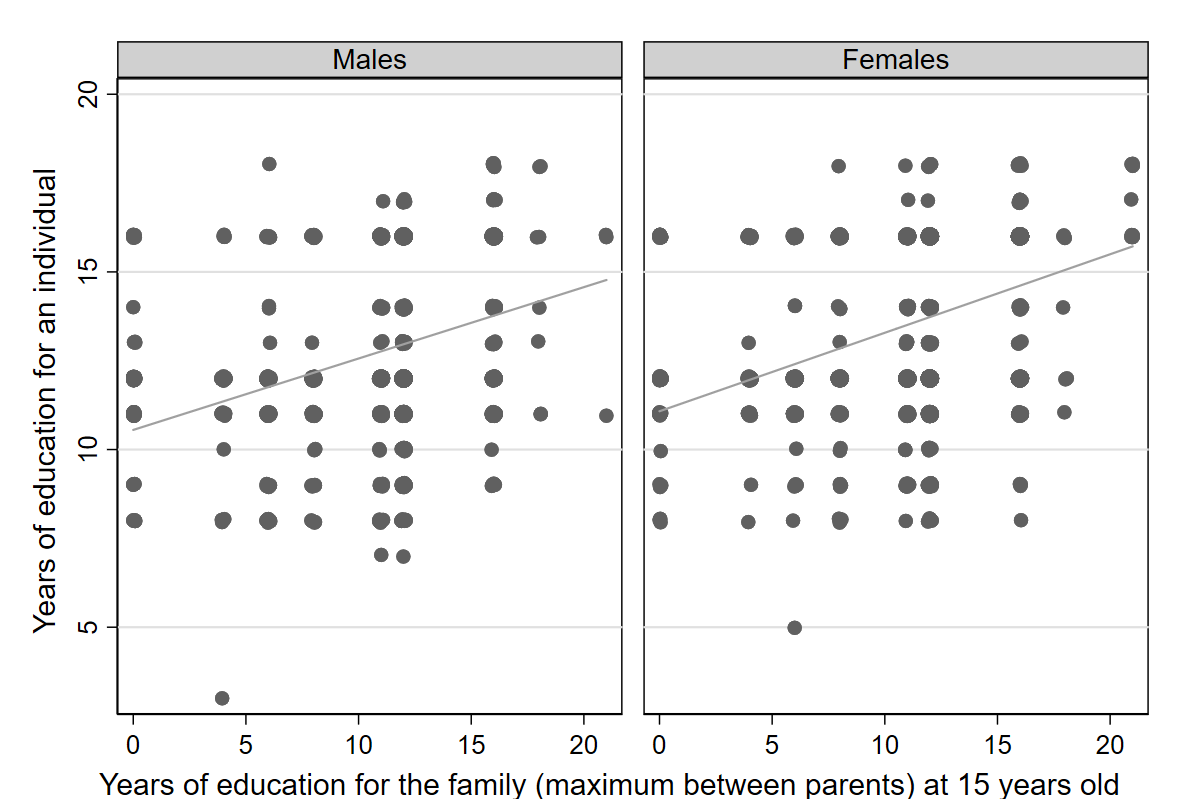
\includegraphics[width=\textwidth]{fam_edu_schooling.png}
	\caption{Individual Years of Education and Family Education Years at 15 Years Old}\label{fig:6.1}
\end{figure}

\begin{figure}[h!]
	\centering
	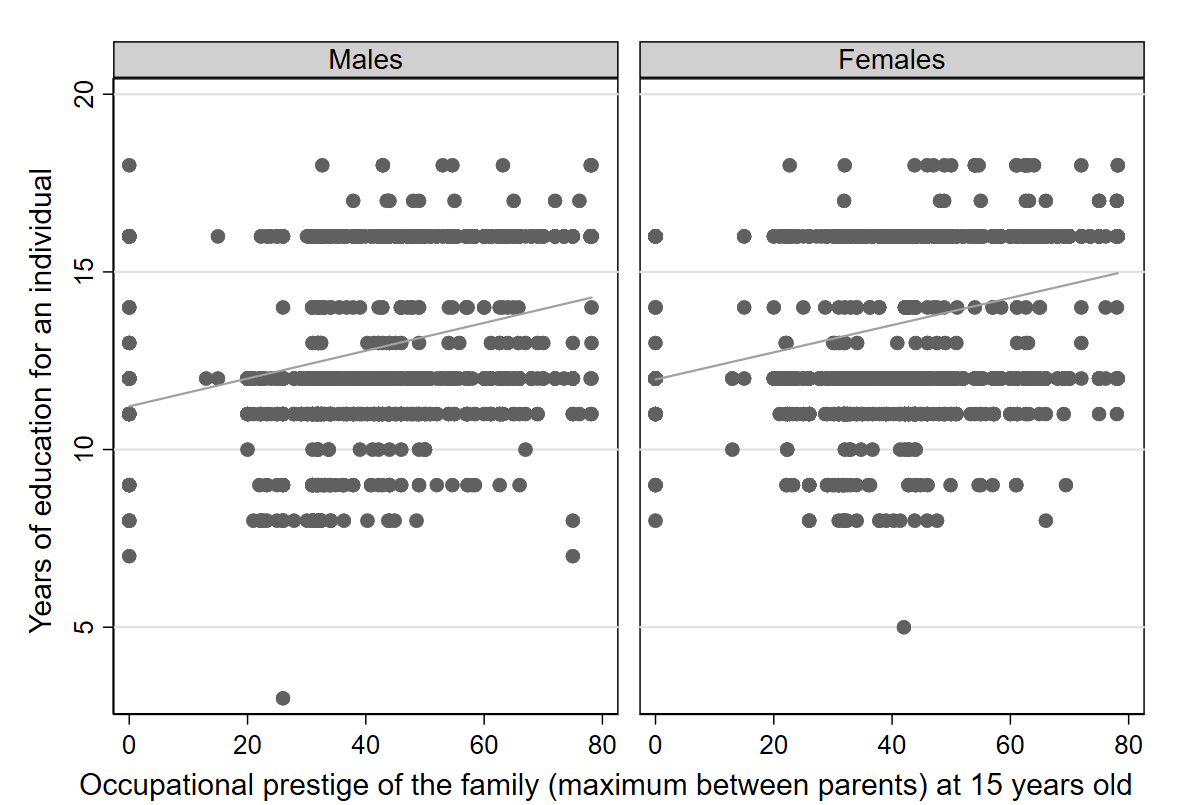
\includegraphics[width=\textwidth]{fam_prestige_schooling.png}
	\caption{Individual Years of Education and Occupational Prestige (SIOPS) of the Family at 15 Years Old}\label{fig:6.2}
\end{figure}

Table \ref{tab:6.1} presents the estimated schooling equation for males and 
females. The results demonstrate that individuals, whose parents had higher 
occupational prestige and more completed years of education, study longer. 
Only statistically significant regional dummies are maintained in the model.

\begin{table}[h!]\centering
	\caption{Schooling Equations: Russia, 2018}
	\label{tab:6.1}
	\begin{tabular}{l*{2}{c}}
		\hline\hline
		&\multicolumn{1}{c}{Females}&\multicolumn{1}{c}{Males}\\
		\hline
		Family occupational prestige &   0.0204&   0.0237\\
		&   (6.65)&   (6.57)\\
		Family education, years &    0.111&   0.0823\\
		&   (7.64)&   (5.01)\\
		Permskiy Krai&   -0.660&   -0.891\\
		&  (-2.78)&  (-3.72)\\
		Tverskaya Oblast&   -0.560&         \\
		&  (-2.31)&         \\
		Krasnoyarskiy Kray&   -1.287&         \\
		&  (-4.32)&         \\
		Rostovskaya Oblast&   -0.825&         \\
		&  (-2.74)&         \\
		Experience     &   -0.120&   -0.153\\
		&  (-8.13)&  (-7.71)\\
		Experience squared    &  0.00129&  0.00198\\
		&   (4.34)&   (5.05)\\
		Urban     &    0.520&    0.795\\
		&   (5.43)&   (7.49)\\
		Tambovskaya Oblast&         &   -0.923\\
		&         &  (-3.92)\\
		Kabardino-Balkarskaya Resp&         &    1.382\\
		&         &   (2.40)\\
		Constant    &    13.18&    12.74\\
		&  (55.35)&  (41.77)\\
		\hline
		\(N\)     &     2222&     1694\\
		\(adj. R^{2}\)&   0.2266      &   0.2359      \\
		F-value &    73.32     &   66.35      \\
		\hline\hline
		\multicolumn{3}{l}{\footnotesize \textit{Note: t} statistics in parentheses}\\
		\multicolumn{3}{l}{\footnotesize  \textit{Source: RLMS}}\\
	\end{tabular}
\end{table}

The IV estimation results, using the parental SES and regional dummies, are shown in Table \ref{tab:6.2}. The instrumental variable approach yields the rate of returns to education in Russia of around 14.3\% for females and 8\% for males. Females' IV parameters appeared to be tangibly larger compared to the respective OLS estimate of 7.6\%, while for males the IV and OLS (6\%) estimates are much closer in magnitude.

\begin{table}[h!]\centering
	\caption{Returns to Education from Instrumental Variables: Russia, 2018}
	\label{tab:6.2}
	\begin{tabular}{l*{2}{c}}
		\hline\hline
		&\multicolumn{1}{c}{Females}&\multicolumn{1}{c}{Males}\\
		\hline
		Education, years   &    0.143&   0.0798\\
		&   (8.19)&   (3.43)\\
		Experience     &   0.0313&   0.0303\\
		&   (5.65)&   (4.30)\\
		Experience squared    &-0.0006 &-0.0007\\
		&  (-5.99)&  (-5.61)\\
		Urban     &    0.161&    0.180\\
		&   (5.51)&   (5.69)\\
		Constant    &    7.501&    8.833\\
		&  (27.00)&  (26.65)\\
		\hline
		\(N\)     &     2222 &     1694\\
		Centered $R^2$  & 0.083   & 0.131 \\
		Partial $R^2$ for excluded instruments in the first stage   & 0.105   &  0.093 \\
		F-test  &  43.63  &  34.43 \\
		\textit{p-value}  &  0.000  & 0.000 \\
		Pagan–Hall for heteroskedasticity  &  5.780   & 9.973 \\
		\textit{p-value}  & 0.762  & 0.267 \\
		Kleibergen-Paap rk LM statistic (underidentification test)  &  200.607  & 132.985 \\
		\textit{p-value}  &  0.000  & 0.000 \\
		Sargan-Hansen J statistic (overidentification test)  & 10.395   & 20.158 \\
		\textit{p-value}  & 0.065   & 0.0005 \\
		Hausman endogeneity test  & 17.243   & 1.099 \\
		\textit{p-value}  & 0.000   & 0.295 \\
		Cragg-Donald Wald F statistic  & 43.279   & 34.399 \\
		\textit{Stock-Yogo critical values: 5\% maximal IV relative bias}  & 19.28   & 18.37 \\
		\textit{Stock-Yogo critical values: 10\% maximal IV size}  & 29.18   & 26.87 \\
		
		\hline\hline
		\multicolumn{3}{l}{\footnotesize  \textit{Note: z} statistics in parentheses}\\
		\multicolumn{3}{l}{\footnotesize  \textit{Source: RLMS}}\\
	\end{tabular}
\end{table}

To ascertain the statistical validity of the implemented instruments we 
conducted an array of diagnostic tests (see Table \ref{tab:6.2}). An F-test 
indicates that the instruments under focus are strongly correlated with the 
endogenous regressor (schooling). Next,  Stock and Yogo's critical values 
test points out that even if we are willing to tolerate a 5\% IV relative 
bias or 10\% IV rejection rate at maximum, our instruments are not weak 
because the Cragg-Donald Wald F statistic in both models exceeds the 
corresponding critical values. The Hausman endogeneity test shows that for 
the sub-sample of males, the education variable does not seem to be 
endogenous ($p>0.05$), therefore, the use of instruments is valid only for 
females. The Sargan-Hansen test also supports this conclusion. Overall, the 
diagnostics contend that the OLS estimates of returns to schooling for 
males in the given specification are more preferable over the IV estimates, 
whereas for females the IV parameters are appropriate.

\section{Conclusions}

Russia is a highly educated country, and the level schooling continues to 
increase. More than one-third of the labor force possesses a post-secondary 
qualification. Our analysis confirms previous studies showing a growth in 
the overall returns to schooling during the post-transition period 
\parencite{Brainerd1998,Clark2003,Vernon2002}. There was an increase in the 
returns to an additional year of schooling in the 1990s. The returns peaked 
in the early 2000s (at almost 10\%), followed by a downward pattern 
(returns of 5.6\%by 2018). The global average is about 8-9\% 
\parencite{Psacharopoulos_Patrinos2018}. The extent to which the declines 
are due to potential "over-education" is worth investigating 
\parencite{Gimpelson2019}.

Education payoffs for women are higher than those of men, but the 
difference appears to have narrowed in recent years. We show that the 
returns to education for females is higher than for males. This is 
consistent with global findings \parencite{Psacharopoulos_Patrinos2018}  
and previous studies of the Russian labor market 
\parencite{Cheidvasser2007,Lukyanova2010}. When estimated separately by 
gender, we find trend variation. The results from estimation of earnings 
functions show that annual returns to higher education for males varied 
from 9\% to 15\%, whereas women's returns are described by an inverse 
U-shaped pattern, reaching their maximum of 28\% in 2003. Within roughly 
the last five years, wage premiums to higher education for women have 
stabilized at around 12\%, a couple of percentage points ahead of men. 
Gender-wise enrollment rates in higher education ten years later appears to 
match the differences in rates of return, strengthening the hypothesis that 
market rates of return to education in Russia do indeed influence 
positively the demand for schooling. Just in the past two years, the 
enrollment decline appears to be slowly reversing, but this phenomenon 
needs to be watched more closely to determine if it is merely a fluctuation 
or a new trend.

We show that private returns to education are three times greater for 
higher education compared to vocational education. On average, wage 
premiums to university education in Russia are roughly 3-5 times greater 
than to vocational schooling. This is consistent with findings from global 
studies and from previous research on the Russian labor market 
\parencite{Borisov2007, Carnoy2012}. Higher education enrollment rates 
increased substantially after the break-up of the Soviet Union 
\parencite{Belskaya2014}. Enrollments peaked in 2009. Subsequent returns to 
higher education started to fall relative to secondary education. The 
latest estimate of the returns to higher education in the Russian 
Federation is about 8\%, which is just below the EU average of about 10\% 
and the global average of 15\%  \parencite{Psacharopoulos_Patrinos2018}. 
But the wage profiles for those with secondary and vocational education is 
almost flat or descending, while the gaps between higher education and 
vocational education are increasing, in favor of higher education. 

Female education is a policy priority. It promotes earnings growth and will help reduce gender gaps in the labor market.  There is a need to investigate the labor market relevance of vocational education given the low and declining returns. Higher education may have reached an expansion limit and it may be necessary to investigate options for increasing the productivity of schooling.

Future research should look at the variations in returns across regions.  Also, it would be useful to estimate social returns to education in order to derive more robust policy recommendations. Finally, causal estimates of the returns to schooling should be estimated.


\printbibliography

\newpage

\pagestyle{empty}
\begin{landscape}


\fontsize{9}{11}
\selectfont

\begin{table}[!htbp] \centering 
\renewcommand{\arraystretch}{1.0}
  \caption{Results of Mincer Analysis, RLMS 1994} 
  \label{} 
\begin{tabular}{@{\extracolsep{5pt}}lcccccc} 
\\[-1.8ex]\hline 
\hline \\[-1.8ex] 
 & Total & Males & Females & Total & Males & Females \\ 
\\[-1.8ex] & (1) & (2) & (3) & (4) & (5) & (6)\\ 
\hline \\[-1.8ex] 
 Constant & 10.905$^{***}$ & 11.265$^{***}$ & 10.449$^{***}$ & 11.570$^{***}$ & 11.946$^{***}$ & 11.134$^{***}$ \\ 
  & (10.679, 11.131) & (10.938, 11.591) & (10.158, 10.740) & (11.387, 11.754) & (11.672, 12.221) & (10.904, 11.364) \\ 
  & & & & & & \\ 
 Education, years & 0.073$^{***}$ & 0.078$^{***}$ & 0.078$^{***}$ &  &  &  \\ 
  & (0.060, 0.087) & (0.058, 0.097) & (0.061, 0.095) &  &  &  \\ 
  & & & & & & \\ 
 Vocational education &  &  &  & 0.115$^{***}$ & 0.132$^{**}$ & 0.158$^{***}$ \\ 
  &  &  &  & (0.030, 0.200) & (0.008, 0.257) & (0.049, 0.268) \\ 
  & & & & & & \\ 
 Higher education &  &  &  & 0.486$^{***}$ & 0.543$^{***}$ & 0.502$^{***}$ \\ 
  &  &  &  & (0.389, 0.583) & (0.400, 0.685) & (0.378, 0.625) \\ 
  & & & & & & \\ 
 Experience & 0.023$^{***}$ & 0.013 & 0.035$^{***}$ & 0.032$^{***}$ & 0.024$^{**}$ & 0.045$^{***}$ \\ 
  & (0.010, 0.036) & ($-$0.007, 0.033) & (0.019, 0.051) & (0.016, 0.047) & (0.001, 0.048) & (0.026, 0.064) \\ 
  & & & & & & \\ 
 Experience squared & $-$0.0004$^{***}$ & $-$0.0003 & $-$0.001$^{***}$ & $-$0.001$^{***}$ & $-$0.001$^{**}$ & $-$0.001$^{***}$ \\ 
  & ($-$0.001, $-$0.0002) & ($-$0.001, 0.0001) & ($-$0.001, $-$0.0003) & ($-$0.001, $-$0.0003) & ($-$0.001, $-$0.0001) & ($-$0.001, $-$0.0005) \\ 
  & & & & & & \\ 
\hline \\[-3ex] 
Observations & 3,204 & 1,487 & 1,717 & 3,041 & 1,395 & 1,646 \\ 
R$^{2}$ & 0.049 & 0.061 & 0.061 & 0.040 & 0.051 & 0.049 \\ 
Adjusted R$^{2}$ & 0.048 & 0.059 & 0.060 & 0.039 & 0.048 & 0.047 \\ 
Residual Std. Error & 0.930 & 0.948 & 0.849 & 0.935 & 0.955 & 0.853 \\ 
F Statistic & 54.847$^{***}$ & 32.176$^{***}$ & 37.217$^{***}$ & 31.859$^{***}$ & 18.578$^{***}$ & 21.336$^{***}$ \\ 
\hline 
\hline \\[-3ex] 
\textit{Note:} &\multicolumn{4}{l}{Figures in parentheses are the limits of the 95\% confidence interval for the coefficient}  & \multicolumn{2}{r}{$^{*}$p$<$0.1; $^{**}$p$<$0.05; $^{***}$p$<$0.01} \\ 
\end{tabular} 
\end{table} 

\end{landscape}

\newpage

\begin{landscape}

\fontsize{9}{11}
\selectfont

\begin{table}[!htbp] \centering 
\renewcommand{\arraystretch}{1.0}
  \caption{Results of Mincer Analysis, RLMS 1995} 
  \label{} 
\begin{tabular}{@{\extracolsep{5pt}}lcccccc} 
\\[-1.8ex]\hline 
\hline \\[-1.8ex] 
 & Total & Males & Females & Total & Males & Females \\ 
\\[-1.8ex] & (1) & (2) & (3) & (4) & (5) & (6)\\ 
\hline \\[-1.8ex] 
 Constant & 11.612$^{***}$ & 12.105$^{***}$ & 11.053$^{***}$ & 12.362$^{***}$ & 12.845$^{***}$ & 11.832$^{***}$ \\ 
  & (11.367, 11.856) & (11.759, 12.450) & (10.726, 11.379) & (12.173, 12.552) & (12.567, 13.122) & (11.585, 12.078) \\ 
  & & & & & & \\ 
 Education, years & 0.076$^{***}$ & 0.073$^{***}$ & 0.085$^{***}$ &  &  &  \\ 
  & (0.061, 0.090) & (0.052, 0.093) & (0.065, 0.104) &  &  &  \\ 
  & & & & & & \\ 
 Vocational education &  &  &  & 0.055 & 0.064 & 0.115$^{*}$ \\ 
  &  &  &  & ($-$0.034, 0.145) & ($-$0.065, 0.193) & ($-$0.004, 0.234) \\ 
  & & & & & & \\ 
 Higher education &  &  &  & 0.421$^{***}$ & 0.397$^{***}$ & 0.503$^{***}$ \\ 
  &  &  &  & (0.322, 0.521) & (0.255, 0.538) & (0.370, 0.635) \\ 
  & & & & & & \\ 
 Experience & 0.024$^{***}$ & 0.007 & 0.043$^{***}$ & 0.032$^{***}$ & 0.012 & 0.055$^{***}$ \\ 
  & (0.010, 0.038) & ($-$0.013, 0.028) & (0.026, 0.061) & (0.016, 0.047) & ($-$0.011, 0.035) & (0.034, 0.075) \\ 
  & & & & & & \\ 
 Experience squared & $-$0.0005$^{***}$ & $-$0.0002 & $-$0.001$^{***}$ & $-$0.001$^{***}$ & $-$0.0004 & $-$0.001$^{***}$ \\ 
  & ($-$0.001, $-$0.0002) & ($-$0.001, 0.0002) & ($-$0.001, $-$0.0005) & ($-$0.001, $-$0.0004) & ($-$0.001, 0.0001) & ($-$0.002, $-$0.001) \\ 
  & & & & & & \\ 
\hline \\[-3ex] 
Observations & 2,792 & 1,293 & 1,499 & 2,693 & 1,237 & 1,456 \\ 
R$^{2}$ & 0.050 & 0.054 & 0.068 & 0.039 & 0.036 & 0.059 \\ 
Adjusted R$^{2}$ & 0.049 & 0.052 & 0.066 & 0.038 & 0.033 & 0.056 \\ 
Residual Std. Error & 0.914 & 0.916 & 0.860 & 0.918 & 0.920 & 0.864 \\ 
F Statistic & 49.270$^{***}$ & 24.594$^{***}$ & 36.509$^{***}$ & 27.447$^{***}$ & 11.576$^{***}$ & 22.579$^{***}$ \\ 
\hline 
\hline \\[-3ex] 
\textit{Note:} &\multicolumn{4}{l}{Figures in parentheses are the limits of the 95\% confidence interval for the coefficient}  & \multicolumn{2}{r}{$^{*}$p$<$0.1; $^{**}$p$<$0.05; $^{***}$p$<$0.01} \\ 
\end{tabular} 
\end{table} 

\end{landscape}

\newpage

\begin{landscape}

\fontsize{9}{11}
\selectfont

\begin{table}[!htbp] \centering 
\renewcommand{\arraystretch}{1.0}
  \caption{Results of Mincer Analysis, RLMS 1996} 
  \label{} 
\begin{tabular}{@{\extracolsep{5pt}}lcccccc} 
\\[-1.8ex]\hline 
\hline \\[-1.8ex] 
 & Total & Males & Females & Total & Males & Females \\ 
\\[-1.8ex] & (1) & (2) & (3) & (4) & (5) & (6)\\ 
\hline \\[-1.8ex] 
 Constant & 12.283$^{***}$ & 12.553$^{***}$ & 11.895$^{***}$ & 12.989$^{***}$ & 13.307$^{***}$ & 12.565$^{***}$ \\ 
  & (12.006, 12.560) & (12.143, 12.963) & (11.541, 12.249) & (12.774, 13.205) & (12.988, 13.626) & (12.290, 12.841) \\ 
  & & & & & & \\ 
 Education, years & 0.070$^{***}$ & 0.076$^{***}$ & 0.071$^{***}$ &  &  &  \\ 
  & (0.053, 0.086) & (0.051, 0.100) & (0.050, 0.092) &  &  &  \\ 
  & & & & & & \\ 
 Vocational education &  &  &  & 0.105$^{*}$ & 0.132$^{*}$ & 0.126$^{*}$ \\ 
  &  &  &  & ($-$0.001, 0.210) & ($-$0.024, 0.287) & ($-$0.009, 0.262) \\ 
  & & & & & & \\ 
 Higher education &  &  &  & 0.377$^{***}$ & 0.400$^{***}$ & 0.411$^{***}$ \\ 
  &  &  &  & (0.262, 0.492) & (0.229, 0.571) & (0.264, 0.558) \\ 
  & & & & & & \\ 
 Experience & 0.002 & $-$0.003 & 0.013 & 0.005 & 0.001 & 0.019$^{*}$ \\ 
  & ($-$0.013, 0.017) & ($-$0.026, 0.020) & ($-$0.005, 0.032) & ($-$0.013, 0.022) & ($-$0.026, 0.027) & ($-$0.003, 0.042) \\ 
  & & & & & & \\ 
 Experience squared & $-$0.0001 & $-$0.0001 & $-$0.0003 & $-$0.0002 & $-$0.0002 & $-$0.0004$^{*}$ \\ 
  & ($-$0.0004, 0.0002) & ($-$0.001, 0.0004) & ($-$0.001, 0.0001) & ($-$0.001, 0.0002) & ($-$0.001, 0.0004) & ($-$0.001, 0.0001) \\ 
    & & & & & & \\ 
  \hline \\[-3ex] 
Observations & 2,355 & 1,067 & 1,288 & 2,283 & 1,034 & 1,249 \\ 
R$^{2}$ & 0.039 & 0.050 & 0.042 & 0.026 & 0.032 & 0.031 \\ 
Adjusted R$^{2}$ & 0.038 & 0.048 & 0.040 & 0.024 & 0.028 & 0.027 \\ 
Residual Std. Error & 0.951 & 0.969 & 0.879 & 0.959 & 0.977 & 0.887 \\ 
F Statistic & 31.838$^{***}$ & 18.765$^{***}$ & 18.779$^{***}$ & 14.947$^{***}$ & 8.405$^{***}$ & 9.812$^{***}$ \\ 
\hline 
\hline \\[-3ex] 
\textit{Note:} &\multicolumn{4}{l}{Figures in parentheses are the limits of the 95\% confidence interval for the coefficient}  & \multicolumn{2}{r}{$^{*}$p$<$0.1; $^{**}$p$<$0.05; $^{***}$p$<$0.01} \\ 
\end{tabular} 
\end{table} 

\end{landscape}

\newpage

\begin{landscape}

\fontsize{9}{11}
\selectfont

\begin{table}[!htbp] \centering 
\renewcommand{\arraystretch}{1.0}
  \caption{Results of Mincer Analysis, RLMS 1998} 
  \label{} 
\begin{tabular}{@{\extracolsep{5pt}}lcccccc} 
\\[-1.8ex]\hline 
\hline \\[-1.8ex] 
 & Total & Males & Females & Total & Males & Females \\ 
\\[-1.8ex] & (1) & (2) & (3) & (4) & (5) & (6)\\ 
\hline \\[-1.8ex] 
 Constant & 5.221$^{***}$ & 5.526$^{***}$ & 4.710$^{***}$ & 5.960$^{***}$ & 6.329$^{***}$ & 5.502$^{***}$ \\ 
  & (5.013, 5.429) & (5.229, 5.823) & (4.443, 4.978) & (5.803, 6.118) & (6.097, 6.561) & (5.304, 5.701) \\ 
  & & & & & & \\ 
 Education, years & 0.084$^{***}$ & 0.090$^{***}$ & 0.094$^{***}$ &  &  &  \\ 
  & (0.071, 0.096) & (0.072, 0.108) & (0.078, 0.110) &  &  &  \\ 
  & & & & & & \\ 
 Vocational education &  &  &  & 0.177$^{***}$ & 0.175$^{***}$ & 0.256$^{***}$ \\ 
  &  &  &  & (0.102, 0.252) & (0.070, 0.280) & (0.157, 0.355) \\ 
  & & & & & & \\ 
 Higher education &  &  &  & 0.527$^{***}$ & 0.552$^{***}$ & 0.616$^{***}$ \\ 
  &  &  &  & (0.443, 0.611) & (0.431, 0.673) & (0.506, 0.725) \\ 
  & & & & & & \\ 
 Experience & 0.019$^{***}$ & 0.008 & 0.032$^{***}$ & 0.028$^{***}$ & 0.019$^{*}$ & 0.043$^{***}$ \\ 
  & (0.007, 0.030) & ($-$0.009, 0.025) & (0.018, 0.046) & (0.015, 0.041) & ($-$0.0001, 0.038) & (0.027, 0.059) \\ 
  & & & & & & \\ 
 Experience squared & $-$0.0004$^{***}$ & $-$0.0002 & $-$0.001$^{***}$ & $-$0.001$^{***}$ & $-$0.0005$^{**}$ & $-$0.001$^{***}$ \\ 
  & ($-$0.001, $-$0.0002) & ($-$0.001, 0.0001) & ($-$0.001, $-$0.0003) & ($-$0.001, $-$0.0003) & ($-$0.001, $-$0.0001) & ($-$0.001, $-$0.001) \\ 
  & & & & & & \\ 
\hline \\[-3ex] 
Observations & 3,186 & 1,483 & 1,703 & 3,108 & 1,438 & 1,670 \\ 
R$^{2}$ & 0.065 & 0.080 & 0.094 & 0.058 & 0.066 & 0.085 \\ 
Adjusted R$^{2}$ & 0.065 & 0.078 & 0.092 & 0.057 & 0.063 & 0.083 \\ 
Residual Std. Error & 0.797 & 0.799 & 0.727 & 0.800 & 0.804 & 0.729 \\ 
F Statistic & 74.330$^{***}$ & 42.686$^{***}$ & 58.475$^{***}$ & 47.544$^{***}$ & 25.234$^{***}$ & 38.908$^{***}$ \\ 
\hline 
\hline \\[-3ex] 
\textit{Note:} &\multicolumn{4}{l}{Figures in parentheses are the limits of the 95\% confidence interval for the coefficient}  & \multicolumn{2}{r}{$^{*}$p$<$0.1; $^{**}$p$<$0.05; $^{***}$p$<$0.01} \\ 
\end{tabular} 
\end{table} 

\end{landscape}

\newpage

\begin{landscape}

\fontsize{9}{11}
\selectfont

\begin{table}[!htbp] \centering 
\renewcommand{\arraystretch}{1.0}
  \caption{Results of Mincer Analysis, RLMS 2000} 
  \label{} 
\begin{tabular}{@{\extracolsep{5pt}}lcccccc} 
\\[-1.8ex]\hline 
\hline \\[-1.8ex] 
 & Total & Males & Females & Total & Males & Females \\ 
\\[-1.8ex] & (1) & (2) & (3) & (4) & (5) & (6)\\ 
\hline \\[-1.8ex] 
 Constant & 5.911$^{***}$ & 6.325$^{***}$ & 5.131$^{***}$ & 6.698$^{***}$ & 7.177$^{***}$ & 6.072$^{***}$ \\ 
  & (5.688, 6.134) & (6.016, 6.635) & (4.835, 5.427) & (6.541, 6.855) & (6.956, 7.399) & (5.869, 6.276) \\ 
  & & & & & & \\ 
 Education, years & 0.084$^{***}$ & 0.086$^{***}$ & 0.105$^{***}$ &  &  &  \\ 
  & (0.070, 0.097) & (0.067, 0.106) & (0.088, 0.122) &  &  &  \\ 
  & & & & & & \\ 
 Vocational education &  &  &  & 0.155$^{***}$ & 0.120$^{**}$ & 0.283$^{***}$ \\ 
  &  &  &  & (0.075, 0.234) & (0.010, 0.230) & (0.178, 0.388) \\ 
  & & & & & & \\ 
 Higher education &  &  &  & 0.488$^{***}$ & 0.450$^{***}$ & 0.668$^{***}$ \\ 
  &  &  &  & (0.399, 0.577) & (0.323, 0.577) & (0.553, 0.784) \\ 
  & & & & & & \\ 
 Experience & 0.015$^{**}$ & 0.003 & 0.036$^{***}$ & 0.021$^{***}$ & 0.010 & 0.042$^{***}$ \\ 
  & (0.003, 0.026) & ($-$0.014, 0.020) & (0.020, 0.051) & (0.008, 0.034) & ($-$0.009, 0.028) & (0.025, 0.058) \\ 
  & & & & & & \\ 
 Experience squared & $-$0.0003$^{**}$ & $-$0.0002 & $-$0.001$^{***}$ & $-$0.0005$^{***}$ & $-$0.0003$^{*}$ & $-$0.001$^{***}$ \\ 
  & ($-$0.001, $-$0.0001) & ($-$0.001, 0.0002) & ($-$0.001, $-$0.0003) & ($-$0.001, $-$0.0002) & ($-$0.001, 0.00005) & ($-$0.001, $-$0.0005) \\ 
  & & & & & & \\ 
\hline \\[-3ex] 
Observations & 3,282 & 1,527 & 1,755 & 3,222 & 1,483 & 1,739 \\ 
R$^{2}$ & 0.051 & 0.069 & 0.084 & 0.044 & 0.046 & 0.082 \\ 
Adjusted R$^{2}$ & 0.050 & 0.067 & 0.082 & 0.043 & 0.044 & 0.080 \\ 
Residual Std. Error & 0.866 & 0.853 & 0.796 & 0.868 & 0.858 & 0.796 \\ 
F Statistic & 58.937$^{***}$ & 37.376$^{***}$ & 53.532$^{***}$ & 36.905$^{***}$ & 17.967$^{***}$ & 38.861$^{***}$ \\ 
\hline 
\hline \\[-3ex] 
\textit{Note:} &\multicolumn{4}{l}{Figures in parentheses are the limits of the 95\% confidence interval for the coefficient}  & \multicolumn{2}{r}{$^{*}$p$<$0.1; $^{**}$p$<$0.05; $^{***}$p$<$0.01} \\ 
\end{tabular} 
\end{table} 

\end{landscape}

\newpage

\begin{landscape}

\fontsize{9}{11}
\selectfont

\begin{table}[!htbp] \centering 
\renewcommand{\arraystretch}{1.0}
  \caption{Results of Mincer Analysis, RLMS 2001} 
  \label{} 
\begin{tabular}{@{\extracolsep{5pt}}lcccccc} 
\\[-1.8ex]\hline 
\hline \\[-1.8ex] 
 & Total & Males & Females & Total & Males & Females \\ 
\\[-1.8ex] & (1) & (2) & (3) & (4) & (5) & (6)\\ 
\hline \\[-1.8ex] 
 Constant & 6.373$^{***}$ & 6.680$^{***}$ & 5.677$^{***}$ & 7.280$^{***}$ & 7.577$^{***}$ & 6.768$^{***}$ \\ 
  & (6.165, 6.581) & (6.388, 6.971) & (5.398, 5.955) & (7.136, 7.424) & (7.373, 7.780) & (6.578, 6.957) \\ 
  & & & & & & \\ 
 Education, years & 0.092$^{***}$ & 0.091$^{***}$ & 0.114$^{***}$ &  &  &  \\ 
  & (0.079, 0.104) & (0.073, 0.109) & (0.098, 0.130) &  &  &  \\ 
  & & & & & & \\ 
 Vocational education &  &  &  & 0.147$^{***}$ & 0.107$^{**}$ & 0.299$^{***}$ \\ 
  &  &  &  & (0.072, 0.221) & (0.004, 0.210) & (0.199, 0.399) \\ 
  & & & & & & \\ 
 Higher education &  &  &  & 0.518$^{***}$ & 0.492$^{***}$ & 0.711$^{***}$ \\ 
  &  &  &  & (0.437, 0.599) & (0.376, 0.608) & (0.603, 0.819) \\ 
  & & & & & & \\ 
 Experience & $-$0.001 & $-$0.003 & 0.012 & 0.003 & 0.005 & 0.012 \\ 
  & ($-$0.012, 0.010) & ($-$0.018, 0.013) & ($-$0.003, 0.027) & ($-$0.009, 0.015) & ($-$0.013, 0.022) & ($-$0.004, 0.028) \\ 
  & & & & & & \\ 
 Experience squared & $-$0.00001 & $-$0.00004 & $-$0.0002 & $-$0.0001 & $-$0.0002 & $-$0.0002 \\ 
  & ($-$0.0002, 0.0002) & ($-$0.0004, 0.0003) & ($-$0.0005, 0.0001) & ($-$0.0004, 0.0001) & ($-$0.001, 0.0001) & ($-$0.001, 0.0002) \\ 
  & & & & & & \\ 
\hline \\[-3ex] 
Observations & 3,659 & 1,708 & 1,951 & 3,611 & 1,675 & 1,936 \\ 
R$^{2}$ & 0.060 & 0.067 & 0.092 & 0.055 & 0.056 & 0.091 \\ 
Adjusted R$^{2}$ & 0.059 & 0.065 & 0.091 & 0.054 & 0.054 & 0.089 \\ 
Residual Std. Error & 0.846 & 0.853 & 0.777 & 0.846 & 0.853 & 0.777 \\ 
F Statistic & 77.748$^{***}$ & 40.535$^{***}$ & 66.139$^{***}$ & 52.342$^{***}$ & 24.825$^{***}$ & 48.381$^{***}$ \\ 
\hline 
\hline \\[-3ex] 
\textit{Note:} &\multicolumn{4}{l}{Figures in parentheses are the limits of the 95\% confidence interval for the coefficient}  & \multicolumn{2}{r}{$^{*}$p$<$0.1; $^{**}$p$<$0.05; $^{***}$p$<$0.01} \\ 
\end{tabular} 
\end{table} 

\end{landscape}

\newpage

\begin{landscape}

\fontsize{9}{11}
\selectfont

\begin{table}[!htbp] \centering 
\renewcommand{\arraystretch}{1.0}
  \caption{Results of Mincer Analysis, RLMS 2002} 
  \label{} 
\begin{tabular}{@{\extracolsep{5pt}}lcccccc} 
\\[-1.8ex]\hline 
\hline \\[-1.8ex] 
 & Total & Males & Females & Total & Males & Females \\ 
\\[-1.8ex] & (1) & (2) & (3) & (4) & (5) & (6)\\ 
\hline \\[-1.8ex] 
 Constant & 6.574$^{***}$ & 6.853$^{***}$ & 5.944$^{***}$ & 7.477$^{***}$ & 7.797$^{***}$ & 6.974$^{***}$ \\ 
  & (6.386, 6.762) & (6.590, 7.116) & (5.693, 6.194) & (7.348, 7.606) & (7.617, 7.978) & (6.802, 7.145) \\ 
  & & & & & & \\ 
 Education, years & 0.091$^{***}$ & 0.094$^{***}$ & 0.111$^{***}$ &  &  &  \\ 
  & (0.080, 0.103) & (0.078, 0.111) & (0.096, 0.125) &  &  &  \\ 
  & & & & & & \\ 
 Vocational education &  &  &  & 0.147$^{***}$ & 0.120$^{**}$ & 0.283$^{***}$ \\ 
  &  &  &  & (0.080, 0.214) & (0.028, 0.211) & (0.191, 0.374) \\ 
  & & & & & & \\ 
 Higher education &  &  &  & 0.510$^{***}$ & 0.496$^{***}$ & 0.687$^{***}$ \\ 
  &  &  &  & (0.437, 0.584) & (0.392, 0.600) & (0.588, 0.785) \\ 
  & & & & & & \\ 
 Experience & 0.014$^{***}$ & 0.010 & 0.025$^{***}$ & 0.018$^{***}$ & 0.016$^{**}$ & 0.027$^{***}$ \\ 
  & (0.004, 0.024) & ($-$0.004, 0.025) & (0.011, 0.038) & (0.007, 0.029) & (0.001, 0.032) & (0.013, 0.042) \\ 
  & & & & & & \\ 
 Experience squared & $-$0.0003$^{***}$ & $-$0.0003$^{**}$ & $-$0.0004$^{***}$ & $-$0.0004$^{***}$ & $-$0.0005$^{***}$ & $-$0.0005$^{***}$ \\ 
  & ($-$0.001, $-$0.0001) & ($-$0.001, $-$0.00003) & ($-$0.001, $-$0.0001) & ($-$0.001, $-$0.0002) & ($-$0.001, $-$0.0001) & ($-$0.001, $-$0.0002) \\ 
  & & & & & & \\ 
\hline \\[-3ex] 
Observations & 3,853 & 1,780 & 2,073 & 3,809 & 1,750 & 2,059 \\ 
R$^{2}$ & 0.069 & 0.087 & 0.100 & 0.060 & 0.068 & 0.098 \\ 
Adjusted R$^{2}$ & 0.068 & 0.086 & 0.099 & 0.059 & 0.066 & 0.097 \\ 
Residual Std. Error & 0.778 & 0.771 & 0.724 & 0.778 & 0.771 & 0.723 \\ 
F Statistic & 95.214$^{***}$ & 56.700$^{***}$ & 76.506$^{***}$ & 61.036$^{***}$ & 31.819$^{***}$ & 56.047$^{***}$ \\ 
\hline 
\hline \\[-3ex] 
\textit{Note:} &\multicolumn{4}{l}{Figures in parentheses are the limits of the 95\% confidence interval for the coefficient}  & \multicolumn{2}{r}{$^{*}$p$<$0.1; $^{**}$p$<$0.05; $^{***}$p$<$0.01} \\ 
\end{tabular} 
\end{table} 

\end{landscape}

\newpage

\begin{landscape}

\fontsize{9}{11}
\selectfont

\begin{table}[!htbp] \centering 
\renewcommand{\arraystretch}{1.0}
  \caption{Results of Mincer Analysis, RLMS 2003} 
  \label{} 
\begin{tabular}{@{\extracolsep{5pt}}lcccccc} 
\\[-1.8ex]\hline 
\hline \\[-1.8ex] 
 & Total & Males & Females & Total & Males & Females \\ 
\\[-1.8ex] & (1) & (2) & (3) & (4) & (5) & (6)\\ 
\hline \\[-1.8ex] 
 Constant & 6.810$^{***}$ & 7.243$^{***}$ & 6.069$^{***}$ & 7.703$^{***}$ & 8.133$^{***}$ & 7.175$^{***}$ \\ 
  & (6.617, 7.004) & (6.973, 7.513) & (5.817, 6.321) & (7.574, 7.832) & (7.951, 8.315) & (7.009, 7.341) \\ 
  & & & & & & \\ 
 Education, years & 0.091$^{***}$ & 0.088$^{***}$ & 0.118$^{***}$ &  &  &  \\ 
  & (0.080, 0.103) & (0.072, 0.105) & (0.104, 0.133) &  &  &  \\ 
  & & & & & & \\ 
 Vocational education &  &  &  & 0.170$^{***}$ & 0.111$^{**}$ & 0.325$^{***}$ \\ 
  &  &  &  & (0.103, 0.237) & (0.020, 0.201) & (0.234, 0.417) \\ 
  & & & & & & \\ 
 Higher education &  &  &  & 0.519$^{***}$ & 0.454$^{***}$ & 0.738$^{***}$ \\ 
  &  &  &  & (0.445, 0.593) & (0.352, 0.556) & (0.640, 0.836) \\ 
  & & & & & & \\ 
 Experience & 0.014$^{***}$ & 0.006 & 0.023$^{***}$ & 0.017$^{***}$ & 0.010 & 0.024$^{***}$ \\ 
  & (0.003, 0.024) & ($-$0.009, 0.021) & (0.010, 0.036) & (0.006, 0.028) & ($-$0.005, 0.026) & (0.010, 0.038) \\ 
  & & & & & & \\ 
 Experience squared & $-$0.0004$^{***}$ & $-$0.0003$^{*}$ & $-$0.0004$^{***}$ & $-$0.0004$^{***}$ & $-$0.0004$^{**}$ & $-$0.0004$^{***}$ \\ 
  & ($-$0.001, $-$0.0001) & ($-$0.001, 0.00003) & ($-$0.001, $-$0.0002) & ($-$0.001, $-$0.0002) & ($-$0.001, $-$0.0001) & ($-$0.001, $-$0.0001) \\ 
  & & & & & & \\ 
\hline \\[-3ex] 
Observations & 3,900 & 1,789 & 2,111 & 3,871 & 1,770 & 2,101 \\ 
R$^{2}$ & 0.071 & 0.084 & 0.112 & 0.064 & 0.069 & 0.109 \\ 
Adjusted R$^{2}$ & 0.071 & 0.082 & 0.111 & 0.063 & 0.067 & 0.107 \\ 
Residual Std. Error & 0.783 & 0.755 & 0.732 & 0.784 & 0.758 & 0.731 \\ 
F Statistic & 99.596$^{***}$ & 54.327$^{***}$ & 88.575$^{***}$ & 66.214$^{***}$ & 32.543$^{***}$ & 64.108$^{***}$ \\ 
\hline 
\hline \\[-3ex] 
\textit{Note:} &\multicolumn{4}{l}{Figures in parentheses are the limits of the 95\% confidence interval for the coefficient}  & \multicolumn{2}{r}{$^{*}$p$<$0.1; $^{**}$p$<$0.05; $^{***}$p$<$0.01} \\ 
\end{tabular} 
\end{table} 

\end{landscape}

\newpage

\begin{landscape}

\fontsize{9}{11}
\selectfont

\begin{table}[!htbp] \centering 
\renewcommand{\arraystretch}{1.0}
  \caption{Results of Mincer Analysis, RLMS 2004} 
  \label{} 
\begin{tabular}{@{\extracolsep{5pt}}lcccccc} 
\\[-1.8ex]\hline 
\hline \\[-1.8ex] 
 & Total & Males & Females & Total & Males & Females \\ 
\\[-1.8ex] & (1) & (2) & (3) & (4) & (5) & (6)\\ 
\hline \\[-1.8ex] 
 Constant & 7.183$^{***}$ & 7.530$^{***}$ & 6.457$^{***}$ & 8.054$^{***}$ & 8.406$^{***}$ & 7.555$^{***}$ \\ 
  & (6.998, 7.367) & (7.276, 7.785) & (6.216, 6.697) & (7.933, 8.176) & (8.235, 8.577) & (7.399, 7.712) \\ 
  & & & & & & \\ 
 Education, years & 0.085$^{***}$ & 0.086$^{***}$ & 0.110$^{***}$ &  &  &  \\ 
  & (0.074, 0.096) & (0.070, 0.101) & (0.096, 0.124) &  &  &  \\ 
  & & & & & & \\ 
 Vocational education &  &  &  & 0.105$^{***}$ & 0.133$^{***}$ & 0.181$^{***}$ \\ 
  &  &  &  & (0.041, 0.169) & (0.048, 0.219) & (0.094, 0.269) \\ 
  & & & & & & \\ 
 Higher education &  &  &  & 0.446$^{***}$ & 0.443$^{***}$ & 0.612$^{***}$ \\ 
  &  &  &  & (0.375, 0.517) & (0.345, 0.541) & (0.518, 0.706) \\ 
  & & & & & & \\ 
 Experience & 0.010$^{*}$ & 0.006 & 0.020$^{***}$ & 0.013$^{**}$ & 0.007 & 0.024$^{***}$ \\ 
  & ($-$0.0001, 0.020) & ($-$0.008, 0.020) & (0.008, 0.033) & (0.002, 0.023) & ($-$0.008, 0.022) & (0.011, 0.037) \\ 
  & & & & & & \\ 
 Experience squared & $-$0.0003$^{***}$ & $-$0.0003$^{**}$ & $-$0.0004$^{***}$ & $-$0.0004$^{***}$ & $-$0.0003$^{**}$ & $-$0.0005$^{***}$ \\ 
  & ($-$0.001, $-$0.0001) & ($-$0.001, $-$0.00003) & ($-$0.001, $-$0.0001) & ($-$0.001, $-$0.0002) & ($-$0.001, $-$0.00004) & ($-$0.001, $-$0.0002) \\ 
  & & & & & & \\ 
\hline \\[-3ex] 
Observations & 3,994 & 1,841 & 2,153 & 3,970 & 1,824 & 2,146 \\ 
R$^{2}$ & 0.072 & 0.096 & 0.108 & 0.062 & 0.074 & 0.100 \\ 
Adjusted R$^{2}$ & 0.072 & 0.094 & 0.107 & 0.061 & 0.072 & 0.099 \\ 
Residual Std. Error & 0.748 & 0.723 & 0.690 & 0.750 & 0.725 & 0.693 \\ 
F Statistic & 103.687$^{***}$ & 64.859$^{***}$ & 86.667$^{***}$ & 65.934$^{***}$ & 36.585$^{***}$ & 59.620$^{***}$ \\ 
\hline 
\hline \\[-3ex] 
\textit{Note:} &\multicolumn{4}{l}{Figures in parentheses are the limits of the 95\% confidence interval for the coefficient}  & \multicolumn{2}{r}{$^{*}$p$<$0.1; $^{**}$p$<$0.05; $^{***}$p$<$0.01} \\ 
\end{tabular} 
\end{table} 

\end{landscape}

\newpage

\begin{landscape}

\fontsize{9}{11}
\selectfont

\begin{table}[!htbp] \centering 
\renewcommand{\arraystretch}{1.0}
  \caption{Results of Mincer Analysis, RLMS 2005} 
  \label{} 
\begin{tabular}{@{\extracolsep{5pt}}lcccccc} 
\\[-1.8ex]\hline 
\hline \\[-1.8ex] 
 & Total & Males & Females & Total & Males & Females \\ 
\\[-1.8ex] & (1) & (2) & (3) & (4) & (5) & (6)\\ 
\hline \\[-1.8ex] 
 Constant & 7.514$^{***}$ & 7.908$^{***}$ & 6.703$^{***}$ & 8.377$^{***}$ & 8.728$^{***}$ & 7.867$^{***}$ \\ 
  & (7.328, 7.699) & (7.651, 8.166) & (6.462, 6.943) & (8.258, 8.496) & (8.561, 8.895) & (7.713, 8.020) \\ 
  & & & & & & \\ 
 Education, years & 0.081$^{***}$ & 0.076$^{***}$ & 0.115$^{***}$ &  &  &  \\ 
  & (0.071, 0.092) & (0.061, 0.092) & (0.101, 0.129) &  &  &  \\ 
  & & & & & & \\ 
 Vocational education &  &  &  & 0.082$^{**}$ & 0.109$^{**}$ & 0.188$^{***}$ \\ 
  &  &  &  & (0.018, 0.146) & (0.024, 0.193) & (0.100, 0.276) \\ 
  & & & & & & \\ 
 Higher education &  &  &  & 0.421$^{***}$ & 0.385$^{***}$ & 0.642$^{***}$ \\ 
  &  &  &  & (0.351, 0.492) & (0.289, 0.482) & (0.548, 0.736) \\ 
  & & & & & & \\ 
 Experience & 0.004 & 0.001 & 0.012$^{**}$ & 0.004 & $-$0.002 & 0.013$^{**}$ \\ 
  & ($-$0.006, 0.013) & ($-$0.013, 0.014) & (0.0003, 0.025) & ($-$0.006, 0.014) & ($-$0.016, 0.012) & (0.0005, 0.026) \\ 
  & & & & & & \\ 
 Experience squared & $-$0.0002$^{*}$ & $-$0.0002 & $-$0.0003$^{**}$ & $-$0.0002$^{*}$ & $-$0.0001 & $-$0.0003$^{**}$ \\ 
  & ($-$0.0004, 0.00001) & ($-$0.0005, 0.0001) & ($-$0.001, $-$0.00002) & ($-$0.0004, 0.00002) & ($-$0.0004, 0.0002) & ($-$0.001, $-$0.00001) \\ 
  & & & & & & \\ 
\hline \\[-3ex] 
Observations & 3,937 & 1,818 & 2,119 & 3,919 & 1,804 & 2,115 \\ 
R$^{2}$ & 0.070 & 0.079 & 0.120 & 0.062 & 0.061 & 0.114 \\ 
Adjusted R$^{2}$ & 0.069 & 0.077 & 0.119 & 0.061 & 0.059 & 0.112 \\ 
Residual Std. Error & 0.745 & 0.720 & 0.685 & 0.745 & 0.719 & 0.686 \\ 
F Statistic & 97.983$^{***}$ & 51.838$^{***}$ & 96.196$^{***}$ & 64.571$^{***}$ & 29.231$^{***}$ & 67.731$^{***}$ \\ 
\hline 
\hline \\[-3ex] 
\textit{Note:} &\multicolumn{4}{l}{Figures in parentheses are the limits of the 95\% confidence interval for the coefficient}  & \multicolumn{2}{r}{$^{*}$p$<$0.1; $^{**}$p$<$0.05; $^{***}$p$<$0.01} \\ 
\end{tabular} 
\end{table} 

\end{landscape}

\newpage

\begin{landscape}

\fontsize{9}{11}
\selectfont

\begin{table}[!htbp] \centering 
\renewcommand{\arraystretch}{1.0}
  \caption{Results of Mincer Analysis, RLMS 2006} 
  \label{} 
\begin{tabular}{@{\extracolsep{5pt}}lcccccc} 
\\[-1.8ex]\hline 
\hline \\[-1.8ex] 
 & Total & Males & Females & Total & Males & Females \\ 
\\[-1.8ex] & (1) & (2) & (3) & (4) & (5) & (6)\\ 
\hline \\[-1.8ex] 
 Constant & 7.750$^{***}$ & 8.083$^{***}$ & 7.026$^{***}$ & 8.590$^{***}$ & 8.875$^{***}$ & 8.164$^{***}$ \\ 
  & (7.590, 7.911) & (7.855, 8.311) & (6.820, 7.231) & (8.486, 8.695) & (8.726, 9.024) & (8.030, 8.298) \\ 
  & & & & & & \\ 
 Education, years & 0.081$^{***}$ & 0.076$^{***}$ & 0.113$^{***}$ &  &  &  \\ 
  & (0.072, 0.090) & (0.063, 0.090) & (0.101, 0.125) &  &  &  \\ 
  & & & & & & \\ 
 Vocational education &  &  &  & 0.081$^{***}$ & 0.091$^{**}$ & 0.197$^{***}$ \\ 
  &  &  &  & (0.025, 0.136) & (0.017, 0.165) & (0.119, 0.274) \\ 
  & & & & & & \\ 
 Higher education &  &  &  & 0.442$^{***}$ & 0.400$^{***}$ & 0.656$^{***}$ \\ 
  &  &  &  & (0.380, 0.504) & (0.315, 0.486) & (0.573, 0.739) \\ 
  & & & & & & \\ 
 Experience & 0.004 & 0.003 & 0.010$^{*}$ & 0.006 & 0.005 & 0.011$^{*}$ \\ 
  & ($-$0.005, 0.012) & ($-$0.009, 0.016) & ($-$0.001, 0.020) & ($-$0.003, 0.015) & ($-$0.008, 0.018) & ($-$0.0001, 0.022) \\ 
  & & & & & & \\ 
 Experience squared & $-$0.0002$^{**}$ & $-$0.0002$^{*}$ & $-$0.0003$^{**}$ & $-$0.0003$^{***}$ & $-$0.0003$^{**}$ & $-$0.0003$^{***}$ \\ 
  & ($-$0.0004, $-$0.00004) & ($-$0.001, 0.00001) & ($-$0.001, $-$0.00005) & ($-$0.0005, $-$0.0001) & ($-$0.001, $-$0.00002) & ($-$0.001, $-$0.0001) \\ 
  & & & & & & \\ 
\hline \\[-3ex] 
Observations & 4,837 & 2,193 & 2,644 & 4,817 & 2,178 & 2,639 \\ 
R$^{2}$ & 0.080 & 0.082 & 0.139 & 0.078 & 0.072 & 0.132 \\ 
Adjusted R$^{2}$ & 0.080 & 0.081 & 0.138 & 0.077 & 0.070 & 0.131 \\ 
Residual Std. Error & 0.719 & 0.698 & 0.666 & 0.716 & 0.691 & 0.668 \\ 
F Statistic & 140.652$^{***}$ & 65.352$^{***}$ & 141.538$^{***}$ & 101.228$^{***}$ & 42.144$^{***}$ & 100.160$^{***}$ \\ 
\hline 
\hline \\[-3ex] 
\textit{Note:} &\multicolumn{4}{l}{Figures in parentheses are the limits of the 95\% confidence interval for the coefficient}  & \multicolumn{2}{r}{$^{*}$p$<$0.1; $^{**}$p$<$0.05; $^{***}$p$<$0.01} \\ 
\end{tabular} 
\end{table} 

\end{landscape}

\newpage

\begin{landscape}

\fontsize{9}{11}
\selectfont

\begin{table}[!htbp] \centering 
\renewcommand{\arraystretch}{1.0}
  \caption{Results of Mincer Analysis, RLMS 2007} 
  \label{} 
\begin{tabular}{@{\extracolsep{5pt}}lcccccc} 
\\[-1.8ex]\hline 
\hline \\[-1.8ex] 
 & Total & Males & Females & Total & Males & Females \\ 
\\[-1.8ex] & (1) & (2) & (3) & (4) & (5) & (6)\\ 
\hline \\[-1.8ex] 
 Constant & 8.178$^{***}$ & 8.526$^{***}$ & 7.480$^{***}$ & 8.830$^{***}$ & 9.075$^{***}$ & 8.461$^{***}$ \\ 
  & (8.025, 8.331) & (8.312, 8.739) & (7.281, 7.680) & (8.731, 8.928) & (8.938, 9.213) & (8.333, 8.588) \\ 
  & & & & & & \\ 
 Education, years & 0.064$^{***}$ & 0.056$^{***}$ & 0.096$^{***}$ &  &  &  \\ 
  & (0.055, 0.073) & (0.044, 0.068) & (0.084, 0.107) &  &  &  \\ 
  & & & & & & \\ 
 Vocational education &  &  &  & 0.082$^{***}$ & 0.139$^{***}$ & 0.132$^{***}$ \\ 
  &  &  &  & (0.029, 0.134) & (0.071, 0.208) & (0.059, 0.205) \\ 
  & & & & & & \\ 
 Higher education &  &  &  & 0.366$^{***}$ & 0.332$^{***}$ & 0.537$^{***}$ \\ 
  &  &  &  & (0.308, 0.424) & (0.253, 0.410) & (0.459, 0.616) \\ 
  & & & & & & \\ 
 Experience & 0.005 & 0.005 & 0.011$^{**}$ & 0.006 & 0.004 & 0.013$^{**}$ \\ 
  & ($-$0.003, 0.013) & ($-$0.007, 0.017) & (0.0003, 0.021) & ($-$0.002, 0.015) & ($-$0.008, 0.016) & (0.002, 0.023) \\ 
  & & & & & & \\ 
 Experience squared & $-$0.0003$^{***}$ & $-$0.0003$^{**}$ & $-$0.0003$^{***}$ & $-$0.0003$^{***}$ & $-$0.0003$^{**}$ & $-$0.0004$^{***}$ \\ 
  & ($-$0.0004, $-$0.0001) & ($-$0.001, $-$0.0001) & ($-$0.001, $-$0.0001) & ($-$0.0005, $-$0.0001) & ($-$0.001, $-$0.00003) & ($-$0.001, $-$0.0002) \\ 
  & & & & & & \\ 
\hline \\[-3ex] 
Observations & 4,766 & 2,174 & 2,592 & 4,747 & 2,161 & 2,586 \\ 
R$^{2}$ & 0.069 & 0.069 & 0.120 & 0.068 & 0.064 & 0.117 \\ 
Adjusted R$^{2}$ & 0.068 & 0.068 & 0.119 & 0.067 & 0.062 & 0.116 \\ 
Residual Std. Error & 0.674 & 0.639 & 0.636 & 0.673 & 0.638 & 0.637 \\ 
F Statistic & 117.382$^{***}$ & 53.847$^{***}$ & 117.362$^{***}$ & 86.858$^{***}$ & 36.710$^{***}$ & 85.757$^{***}$ \\ 
\hline 
\hline \\[-3ex] 
\textit{Note:} &\multicolumn{4}{l}{Figures in parentheses are the limits of the 95\% confidence interval for the coefficient}  & \multicolumn{2}{r}{$^{*}$p$<$0.1; $^{**}$p$<$0.05; $^{***}$p$<$0.01} \\ 
\end{tabular} 
\end{table} 

\end{landscape}

\newpage

\begin{landscape}

\fontsize{9}{11}
\selectfont

\begin{table}[!htbp] \centering 
\renewcommand{\arraystretch}{1.0}
  \caption{Results of Mincer Analysis, RLMS 2008} 
  \label{} 
\begin{tabular}{@{\extracolsep{5pt}}lcccccc} 
\\[-1.8ex]\hline 
\hline \\[-1.8ex] 
 & Total & Males & Females & Total & Males & Females \\ 
\\[-1.8ex] & (1) & (2) & (3) & (4) & (5) & (6)\\ 
\hline \\[-1.8ex] 
 Constant & 8.133$^{***}$ & 8.386$^{***}$ & 7.477$^{***}$ & 8.915$^{***}$ & 9.145$^{***}$ & 8.545$^{***}$ \\ 
  & (7.970, 8.296) & (8.156, 8.616) & (7.265, 7.689) & (8.811, 9.019) & (8.999, 9.291) & (8.410, 8.680) \\ 
  & & & & & & \\ 
 Education, years & 0.079$^{***}$ & 0.078$^{***}$ & 0.108$^{***}$ &  &  &  \\ 
  & (0.069, 0.088) & (0.065, 0.091) & (0.096, 0.120) &  &  &  \\ 
  & & & & & & \\ 
 Vocational education &  &  &  & 0.097$^{***}$ & 0.134$^{***}$ & 0.177$^{***}$ \\ 
  &  &  &  & (0.040, 0.153) & (0.061, 0.206) & (0.098, 0.256) \\ 
  & & & & & & \\ 
 Higher education &  &  &  & 0.442$^{***}$ & 0.453$^{***}$ & 0.608$^{***}$ \\ 
  &  &  &  & (0.381, 0.504) & (0.370, 0.536) & (0.524, 0.692) \\ 
  & & & & & & \\ 
 Experience & 0.016$^{***}$ & 0.019$^{***}$ & 0.018$^{***}$ & 0.018$^{***}$ & 0.020$^{***}$ & 0.020$^{***}$ \\ 
  & (0.007, 0.024) & (0.007, 0.031) & (0.007, 0.028) & (0.010, 0.027) & (0.008, 0.033) & (0.010, 0.031) \\ 
  & & & & & & \\ 
 Experience squared & $-$0.0005$^{***}$ & $-$0.001$^{***}$ & $-$0.0005$^{***}$ & $-$0.001$^{***}$ & $-$0.001$^{***}$ & $-$0.0005$^{***}$ \\ 
  & ($-$0.001, $-$0.0003) & ($-$0.001, $-$0.0003) & ($-$0.001, $-$0.0002) & ($-$0.001, $-$0.0004) & ($-$0.001, $-$0.0004) & ($-$0.001, $-$0.0003) \\ 
  & & & & & & \\ 
\hline \\[-3ex] 
Observations & 4,844 & 2,182 & 2,662 & 4,832 & 2,172 & 2,660 \\ 
R$^{2}$ & 0.084 & 0.100 & 0.126 & 0.082 & 0.096 & 0.118 \\ 
Adjusted R$^{2}$ & 0.084 & 0.099 & 0.125 & 0.082 & 0.094 & 0.117 \\ 
Residual Std. Error & 0.715 & 0.674 & 0.679 & 0.715 & 0.674 & 0.682 \\ 
F Statistic & 148.108$^{***}$ & 81.005$^{***}$ & 127.729$^{***}$ & 108.415$^{***}$ & 57.530$^{***}$ & 88.839$^{***}$ \\ 
\hline 
\hline \\[-3ex] 
\textit{Note:} &\multicolumn{4}{l}{Figures in parentheses are the limits of the 95\% confidence interval for the coefficient}  & \multicolumn{2}{r}{$^{*}$p$<$0.1; $^{**}$p$<$0.05; $^{***}$p$<$0.01} \\ 
\end{tabular} 
\end{table} 

\end{landscape}

\newpage

\begin{landscape}

\fontsize{9}{11}
\selectfont

\begin{table}[!htbp] \centering 
\renewcommand{\arraystretch}{1.0}
  \caption{Results of Mincer Analysis, RLMS 2009} 
  \label{} 
\begin{tabular}{@{\extracolsep{5pt}}lcccccc} 
\\[-1.8ex]\hline 
\hline \\[-1.8ex] 
 & Total & Males & Females & Total & Males & Females \\ 
\\[-1.8ex] & (1) & (2) & (3) & (4) & (5) & (6)\\ 
\hline \\[-1.8ex] 
 Constant & 8.183$^{***}$ & 8.527$^{***}$ & 7.461$^{***}$ & 8.930$^{***}$ & 9.214$^{***}$ & 8.511$^{***}$ \\ 
  & (8.027, 8.339) & (8.310, 8.744) & (7.257, 7.666) & (8.831, 9.030) & (9.076, 9.351) & (8.380, 8.642) \\ 
  & & & & & & \\ 
 Education, years & 0.075$^{***}$ & 0.070$^{***}$ & 0.106$^{***}$ &  &  &  \\ 
  & (0.067, 0.084) & (0.058, 0.083) & (0.095, 0.118) &  &  &  \\ 
  & & & & & & \\ 
 Vocational education &  &  &  & 0.093$^{***}$ & 0.098$^{***}$ & 0.177$^{***}$ \\ 
  &  &  &  & (0.038, 0.148) & (0.027, 0.169) & (0.099, 0.254) \\ 
  & & & & & & \\ 
 Higher education &  &  &  & 0.422$^{***}$ & 0.404$^{***}$ & 0.597$^{***}$ \\ 
  &  &  &  & (0.363, 0.482) & (0.323, 0.484) & (0.516, 0.679) \\ 
  & & & & & & \\ 
 Experience & 0.019$^{***}$ & 0.018$^{***}$ & 0.026$^{***}$ & 0.022$^{***}$ & 0.020$^{***}$ & 0.029$^{***}$ \\ 
  & (0.011, 0.027) & (0.006, 0.029) & (0.016, 0.036) & (0.014, 0.030) & (0.009, 0.031) & (0.019, 0.039) \\ 
  & & & & & & \\ 
 Experience squared & $-$0.001$^{***}$ & $-$0.001$^{***}$ & $-$0.001$^{***}$ & $-$0.001$^{***}$ & $-$0.001$^{***}$ & $-$0.001$^{***}$ \\ 
  & ($-$0.001, $-$0.0004) & ($-$0.001, $-$0.0003) & ($-$0.001, $-$0.0004) & ($-$0.001, $-$0.0004) & ($-$0.001, $-$0.0003) & ($-$0.001, $-$0.0004) \\ 
  & & & & & & \\ 
\hline \\[-3ex] 
Observations & 4,818 & 2,155 & 2,663 & 4,808 & 2,150 & 2,658 \\ 
R$^{2}$ & 0.080 & 0.092 & 0.128 & 0.078 & 0.089 & 0.118 \\ 
Adjusted R$^{2}$ & 0.080 & 0.090 & 0.127 & 0.077 & 0.088 & 0.117 \\ 
Residual Std. Error & 0.681 & 0.636 & 0.651 & 0.681 & 0.636 & 0.655 \\ 
F Statistic & 139.709$^{***}$ & 72.368$^{***}$ & 129.693$^{***}$ & 101.856$^{***}$ & 52.583$^{***}$ & 88.717$^{***}$ \\ 
\hline 
\hline \\[-3ex] 
\textit{Note:} &\multicolumn{4}{l}{Figures in parentheses are the limits of the 95\% confidence interval for the coefficient}  & \multicolumn{2}{r}{$^{*}$p$<$0.1; $^{**}$p$<$0.05; $^{***}$p$<$0.01} \\ 
\end{tabular} 
\end{table} 

\end{landscape}

\newpage

\begin{landscape}

\fontsize{9}{11}
\selectfont

\begin{table}[!htbp] \centering 
\renewcommand{\arraystretch}{1.0}
  \caption{Results of Mincer Analysis, RLMS 2010} 
  \label{} 
\begin{tabular}{@{\extracolsep{5pt}}lcccccc} 
\\[-1.8ex]\hline 
\hline \\[-1.8ex] 
 & Total & Males & Females & Total & Males & Females \\ 
\\[-1.8ex] & (1) & (2) & (3) & (4) & (5) & (6)\\ 
\hline \\[-1.8ex] 
 Constant & 8.416$^{***}$ & 8.596$^{***}$ & 7.826$^{***}$ & 9.146$^{***}$ & 9.321$^{***}$ & 8.809$^{***}$ \\ 
  & (8.292, 8.540) & (8.420, 8.771) & (7.664, 7.988) & (9.068, 9.224) & (9.210, 9.432) & (8.708, 8.910) \\ 
  & & & & & & \\ 
 Education, years & 0.070$^{***}$ & 0.072$^{***}$ & 0.094$^{***}$ &  &  &  \\ 
  & (0.063, 0.077) & (0.062, 0.082) & (0.085, 0.104) &  &  &  \\ 
  & & & & & & \\ 
 Vocational education &  &  &  & 0.061$^{***}$ & 0.111$^{***}$ & 0.115$^{***}$ \\ 
  &  &  &  & (0.017, 0.104) & (0.054, 0.169) & (0.054, 0.176) \\ 
  & & & & & & \\ 
 Higher education &  &  &  & 0.383$^{***}$ & 0.414$^{***}$ & 0.514$^{***}$ \\ 
  &  &  &  & (0.336, 0.430) & (0.349, 0.479) & (0.450, 0.579) \\ 
  & & & & & & \\ 
 Experience & 0.012$^{***}$ & 0.017$^{***}$ & 0.015$^{***}$ & 0.014$^{***}$ & 0.018$^{***}$ & 0.016$^{***}$ \\ 
  & (0.006, 0.018) & (0.008, 0.026) & (0.007, 0.023) & (0.007, 0.020) & (0.009, 0.028) & (0.008, 0.024) \\ 
  & & & & & & \\ 
 Experience squared & $-$0.0004$^{***}$ & $-$0.001$^{***}$ & $-$0.0004$^{***}$ & $-$0.0004$^{***}$ & $-$0.001$^{***}$ & $-$0.0004$^{***}$ \\ 
  & ($-$0.001, $-$0.0003) & ($-$0.001, $-$0.0004) & ($-$0.001, $-$0.0002) & ($-$0.001, $-$0.0003) & ($-$0.001, $-$0.0004) & ($-$0.001, $-$0.0002) \\ 
  & & & & & & \\ 
\hline \\[-3ex] 
Observations & 7,360 & 3,339 & 4,021 & 7,341 & 3,325 & 4,016 \\ 
R$^{2}$ & 0.077 & 0.099 & 0.110 & 0.076 & 0.094 & 0.106 \\ 
Adjusted R$^{2}$ & 0.076 & 0.098 & 0.110 & 0.076 & 0.093 & 0.105 \\ 
Residual Std. Error & 0.674 & 0.651 & 0.632 & 0.673 & 0.652 & 0.634 \\ 
F Statistic & 204.097$^{***}$ & 122.160$^{***}$ & 165.996$^{***}$ & 151.744$^{***}$ & 85.825$^{***}$ & 119.134$^{***}$ \\ 
\hline 
\hline \\[-3ex] 
\textit{Note:} &\multicolumn{4}{l}{Figures in parentheses are the limits of the 95\% confidence interval for the coefficient}  & \multicolumn{2}{r}{$^{*}$p$<$0.1; $^{**}$p$<$0.05; $^{***}$p$<$0.01} \\ 
\end{tabular} 
\end{table} 

\end{landscape}

\newpage

\begin{landscape}

\fontsize{9}{11}
\selectfont

\begin{table}[!htbp] \centering 
\renewcommand{\arraystretch}{1.0}
  \caption{Results of Mincer Analysis, RLMS 2011} 
  \label{} 
\begin{tabular}{@{\extracolsep{5pt}}lcccccc} 
\\[-1.8ex]\hline 
\hline \\[-1.8ex] 
 & Total & Males & Females & Total & Males & Females \\ 
\\[-1.8ex] & (1) & (2) & (3) & (4) & (5) & (6)\\ 
\hline \\[-1.8ex] 
 Constant & 8.579$^{***}$ & 8.692$^{***}$ & 7.971$^{***}$ & 9.303$^{***}$ & 9.460$^{***}$ & 8.954$^{***}$ \\ 
  & (8.457, 8.702) & (8.527, 8.857) & (7.807, 8.135) & (9.227, 9.379) & (9.358, 9.562) & (8.853, 9.056) \\ 
  & & & & & & \\ 
 Education, years & 0.066$^{***}$ & 0.074$^{***}$ & 0.090$^{***}$ &  &  &  \\ 
  & (0.059, 0.073) & (0.064, 0.083) & (0.080, 0.099) &  &  &  \\ 
  & & & & & & \\ 
 Vocational education &  &  &  & 0.009 & 0.086$^{***}$ & 0.042 \\ 
  &  &  &  & ($-$0.033, 0.051) & (0.033, 0.139) & ($-$0.018, 0.102) \\ 
  & & & & & & \\ 
 Higher education &  &  &  & 0.326$^{***}$ & 0.399$^{***}$ & 0.438$^{***}$ \\ 
  &  &  &  & (0.280, 0.371) & (0.339, 0.459) & (0.374, 0.501) \\ 
  & & & & & & \\ 
 Experience & 0.014$^{***}$ & 0.020$^{***}$ & 0.017$^{***}$ & 0.016$^{***}$ & 0.021$^{***}$ & 0.019$^{***}$ \\ 
  & (0.008, 0.020) & (0.011, 0.028) & (0.010, 0.025) & (0.009, 0.022) & (0.012, 0.029) & (0.011, 0.027) \\ 
  & & & & & & \\ 
 Experience squared & $-$0.0005$^{***}$ & $-$0.001$^{***}$ & $-$0.0004$^{***}$ & $-$0.0005$^{***}$ & $-$0.001$^{***}$ & $-$0.0005$^{***}$ \\ 
  & ($-$0.001, $-$0.0003) & ($-$0.001, $-$0.0004) & ($-$0.001, $-$0.0003) & ($-$0.001, $-$0.0004) & ($-$0.001, $-$0.0005) & ($-$0.001, $-$0.0003) \\ 
  & & & & & & \\ 
\hline \\[-3ex] 
Observations & 7,197 & 3,287 & 3,910 & 7,181 & 3,274 & 3,907 \\ 
R$^{2}$ & 0.086 & 0.125 & 0.112 & 0.085 & 0.117 & 0.106 \\ 
Adjusted R$^{2}$ & 0.085 & 0.124 & 0.112 & 0.084 & 0.116 & 0.105 \\ 
Residual Std. Error & 0.652 & 0.599 & 0.623 & 0.653 & 0.600 & 0.625 \\ 
F Statistic & 225.034$^{***}$ & 155.765$^{***}$ & 164.526$^{***}$ & 165.664$^{***}$ & 108.723$^{***}$ & 115.528$^{***}$ \\ 
\hline 
\hline \\[-3ex] 
\textit{Note:} &\multicolumn{4}{l}{Figures in parentheses are the limits of the 95\% confidence interval for the coefficient}  & \multicolumn{2}{r}{$^{*}$p$<$0.1; $^{**}$p$<$0.05; $^{***}$p$<$0.01} \\ 
\end{tabular} 
\end{table} 

\end{landscape}

\newpage

\begin{landscape}

\fontsize{9}{11}
\selectfont

\begin{table}[!htbp] \centering 
\renewcommand{\arraystretch}{1.0}
  \caption{Results of Mincer Analysis, RLMS 2012} 
  \label{} 
\begin{tabular}{@{\extracolsep{5pt}}lcccccc} 
\\[-1.8ex]\hline 
\hline \\[-1.8ex] 
 & Total & Males & Females & Total & Males & Females \\ 
\\[-1.8ex] & (1) & (2) & (3) & (4) & (5) & (6)\\ 
\hline \\[-1.8ex] 
 Constant & 8.788$^{***}$ & 8.914$^{***}$ & 8.159$^{***}$ & 9.456$^{***}$ & 9.616$^{***}$ & 9.104$^{***}$ \\ 
  & (8.667, 8.909) & (8.753, 9.076) & (7.999, 8.320) & (9.380, 9.531) & (9.515, 9.717) & (9.004, 9.205) \\ 
  & & & & & & \\ 
 Education, years & 0.061$^{***}$ & 0.068$^{***}$ & 0.085$^{***}$ &  &  &  \\ 
  & (0.054, 0.067) & (0.058, 0.077) & (0.077, 0.094) &  &  &  \\ 
  & & & & & & \\ 
 Vocational education &  &  &  & $-$0.007 & 0.079$^{***}$ & 0.015 \\ 
  &  &  &  & ($-$0.049, 0.035) & (0.027, 0.131) & ($-$0.045, 0.076) \\ 
  & & & & & & \\ 
 Higher education &  &  &  & 0.298$^{***}$ & 0.373$^{***}$ & 0.412$^{***}$ \\ 
  &  &  &  & (0.252, 0.343) & (0.315, 0.432) & (0.349, 0.475) \\ 
  & & & & & & \\ 
 Experience & 0.017$^{***}$ & 0.026$^{***}$ & 0.019$^{***}$ & 0.018$^{***}$ & 0.026$^{***}$ & 0.020$^{***}$ \\ 
  & (0.011, 0.023) & (0.018, 0.035) & (0.011, 0.026) & (0.012, 0.025) & (0.018, 0.035) & (0.012, 0.028) \\ 
  & & & & & & \\ 
 Experience squared & $-$0.001$^{***}$ & $-$0.001$^{***}$ & $-$0.0005$^{***}$ & $-$0.001$^{***}$ & $-$0.001$^{***}$ & $-$0.0005$^{***}$ \\ 
  & ($-$0.001, $-$0.0004) & ($-$0.001, $-$0.001) & ($-$0.001, $-$0.0003) & ($-$0.001, $-$0.0005) & ($-$0.001, $-$0.001) & ($-$0.001, $-$0.0003) \\ 
  & & & & & & \\ 
\hline \\[-3ex] 
Observations & 7,461 & 3,385 & 4,076 & 7,442 & 3,371 & 4,071 \\ 
R$^{2}$ & 0.087 & 0.150 & 0.104 & 0.087 & 0.145 & 0.099 \\ 
Adjusted R$^{2}$ & 0.086 & 0.149 & 0.103 & 0.086 & 0.144 & 0.098 \\ 
Residual Std. Error & 0.668 & 0.602 & 0.643 & 0.668 & 0.603 & 0.644 \\ 
F Statistic & 236.314$^{***}$ & 198.539$^{***}$ & 157.757$^{***}$ & 176.856$^{***}$ & 143.027$^{***}$ & 111.637$^{***}$ \\ 
\hline 
\hline \\[-3ex] 
\textit{Note:} &\multicolumn{4}{l}{Figures in parentheses are the limits of the 95\% confidence interval for the coefficient}  & \multicolumn{2}{r}{$^{*}$p$<$0.1; $^{**}$p$<$0.05; $^{***}$p$<$0.01} \\ 
\end{tabular} 
\end{table} 

\end{landscape}

\newpage

\begin{landscape}

\fontsize{9}{11}
\selectfont

\begin{table}[!htbp] \centering 
\renewcommand{\arraystretch}{1.0}
  \caption{Results of Mincer Analysis, RLMS 2013} 
  \label{} 
\begin{tabular}{@{\extracolsep{5pt}}lcccccc} 
\\[-1.8ex]\hline 
\hline \\[-1.8ex] 
 & Total & Males & Females & Total & Males & Females \\ 
\\[-1.8ex] & (1) & (2) & (3) & (4) & (5) & (6)\\ 
\hline \\[-1.8ex] 
 Constant & 8.793$^{***}$ & 9.014$^{***}$ & 8.095$^{***}$ & 9.497$^{***}$ & 9.713$^{***}$ & 9.094$^{***}$ \\ 
  & (8.671, 8.916) & (8.847, 9.182) & (7.932, 8.259) & (9.420, 9.574) & (9.609, 9.817) & (8.991, 9.196) \\ 
  & & & & & & \\ 
 Education, years & 0.065$^{***}$ & 0.067$^{***}$ & 0.094$^{***}$ &  &  &  \\ 
  & (0.058, 0.072) & (0.057, 0.076) & (0.085, 0.103) &  &  &  \\ 
  & & & & & & \\ 
 Vocational education &  &  &  & 0.011 & 0.050$^{*}$ & 0.082$^{**}$ \\ 
  &  &  &  & ($-$0.032, 0.054) & ($-$0.003, 0.103) & (0.020, 0.144) \\ 
  & & & & & & \\ 
 Higher education &  &  &  & 0.329$^{***}$ & 0.353$^{***}$ & 0.501$^{***}$ \\ 
  &  &  &  & (0.283, 0.375) & (0.292, 0.414) & (0.437, 0.566) \\ 
  & & & & & & \\ 
 Experience & 0.019$^{***}$ & 0.022$^{***}$ & 0.023$^{***}$ & 0.020$^{***}$ & 0.024$^{***}$ & 0.024$^{***}$ \\ 
  & (0.013, 0.025) & (0.014, 0.031) & (0.015, 0.031) & (0.014, 0.027) & (0.015, 0.033) & (0.016, 0.032) \\ 
  & & & & & & \\ 
 Experience squared & $-$0.001$^{***}$ & $-$0.001$^{***}$ & $-$0.001$^{***}$ & $-$0.001$^{***}$ & $-$0.001$^{***}$ & $-$0.001$^{***}$ \\ 
  & ($-$0.001, $-$0.0005) & ($-$0.001, $-$0.001) & ($-$0.001, $-$0.0004) & ($-$0.001, $-$0.0005) & ($-$0.001, $-$0.001) & ($-$0.001, $-$0.0004) \\ 
  & & & & & & \\ 
\hline \\[-3ex] 
Observations & 7,346 & 3,368 & 3,978 & 7,332 & 3,358 & 3,974 \\ 
R$^{2}$ & 0.092 & 0.136 & 0.122 & 0.093 & 0.133 & 0.121 \\ 
Adjusted R$^{2}$ & 0.092 & 0.135 & 0.121 & 0.092 & 0.131 & 0.120 \\ 
Residual Std. Error & 0.657 & 0.608 & 0.629 & 0.657 & 0.609 & 0.630 \\ 
F Statistic & 247.588$^{***}$ & 176.036$^{***}$ & 184.225$^{***}$ & 187.572$^{***}$ & 128.051$^{***}$ & 136.169$^{***}$ \\ 
\hline 
\hline \\[-3ex] 
\textit{Note:} &\multicolumn{4}{l}{Figures in parentheses are the limits of the 95\% confidence interval for the coefficient}  & \multicolumn{2}{r}{$^{*}$p$<$0.1; $^{**}$p$<$0.05; $^{***}$p$<$0.01} \\ 
\end{tabular} 
\end{table} 

\end{landscape}

\newpage

\begin{landscape}

\fontsize{9}{11}
\selectfont

\begin{table}[!htbp] \centering 
\renewcommand{\arraystretch}{1.0}
  \caption{Results of Mincer Analysis, RLMS 2014} 
  \label{} 
\begin{tabular}{@{\extracolsep{5pt}}lcccccc} 
\\[-1.8ex]\hline 
\hline \\[-1.8ex] 
 & Total & Males & Females & Total & Males & Females \\ 
\\[-1.8ex] & (1) & (2) & (3) & (4) & (5) & (6)\\ 
\hline \\[-1.8ex] 
 Constant & 8.816$^{***}$ & 8.969$^{***}$ & 8.170$^{***}$ & 9.571$^{***}$ & 9.729$^{***}$ & 9.225$^{***}$ \\ 
  & (8.684, 8.947) & (8.783, 9.156) & (7.999, 8.342) & (9.488, 9.653) & (9.613, 9.845) & (9.117, 9.333) \\ 
  & & & & & & \\ 
 Education, years & 0.068$^{***}$ & 0.072$^{***}$ & 0.096$^{***}$ &  &  &  \\ 
  & (0.061, 0.076) & (0.061, 0.082) & (0.087, 0.106) &  &  &  \\ 
  & & & & & & \\ 
 Vocational education &  &  &  & 0.008 & 0.058$^{*}$ & 0.068$^{**}$ \\ 
  &  &  &  & ($-$0.038, 0.054) & ($-$0.002, 0.117) & (0.002, 0.134) \\ 
  & & & & & & \\ 
 Higher education &  &  &  & 0.335$^{***}$ & 0.378$^{***}$ & 0.487$^{***}$ \\ 
  &  &  &  & (0.286, 0.384) & (0.311, 0.446) & (0.419, 0.556) \\ 
  & & & & & & \\ 
 Experience & 0.021$^{***}$ & 0.026$^{***}$ & 0.024$^{***}$ & 0.022$^{***}$ & 0.027$^{***}$ & 0.024$^{***}$ \\ 
  & (0.015, 0.028) & (0.017, 0.035) & (0.016, 0.033) & (0.016, 0.029) & (0.018, 0.037) & (0.016, 0.033) \\ 
  & & & & & & \\ 
 Experience squared & $-$0.001$^{***}$ & $-$0.001$^{***}$ & $-$0.001$^{***}$ & $-$0.001$^{***}$ & $-$0.001$^{***}$ & $-$0.001$^{***}$ \\ 
  & ($-$0.001, $-$0.0005) & ($-$0.001, $-$0.001) & ($-$0.001, $-$0.0004) & ($-$0.001, $-$0.0005) & ($-$0.001, $-$0.001) & ($-$0.001, $-$0.0004) \\ 
  & & & & & & \\ 
\hline \\[-3ex] 
Observations & 6,161 & 2,803 & 3,358 & 6,150 & 2,793 & 3,357 \\ 
R$^{2}$ & 0.094 & 0.124 & 0.134 & 0.094 & 0.120 & 0.128 \\ 
Adjusted R$^{2}$ & 0.094 & 0.123 & 0.133 & 0.093 & 0.118 & 0.127 \\ 
Residual Std. Error & 0.641 & 0.615 & 0.600 & 0.641 & 0.616 & 0.602 \\ 
F Statistic & 212.827$^{***}$ & 132.356$^{***}$ & 172.860$^{***}$ & 158.634$^{***}$ & 94.659$^{***}$ & 123.316$^{***}$ \\ 
\hline 
\hline \\[-3ex] 
\textit{Note:} &\multicolumn{4}{l}{Figures in parentheses are the limits of the 95\% confidence interval for the coefficient}  & \multicolumn{2}{r}{$^{*}$p$<$0.1; $^{**}$p$<$0.05; $^{***}$p$<$0.01} \\ 
\end{tabular} 
\end{table} 

\end{landscape}

\newpage

\begin{landscape}

\fontsize{9}{11}
\selectfont

\begin{table}[!htbp] \centering 
\renewcommand{\arraystretch}{1.0}
  \caption{Results of Mincer Analysis, RLMS 2015} 
  \label{} 
\begin{tabular}{@{\extracolsep{5pt}}lcccccc} 
\\[-1.8ex]\hline 
\hline \\[-1.8ex] 
 & Total & Males & Females & Total & Males & Females \\ 
\\[-1.8ex] & (1) & (2) & (3) & (4) & (5) & (6)\\ 
\hline \\[-1.8ex] 
 Constant & 9.052$^{***}$ & 9.101$^{***}$ & 8.484$^{***}$ & 9.656$^{***}$ & 9.764$^{***}$ & 9.348$^{***}$ \\ 
  & (8.923, 9.181) & (8.927, 9.276) & (8.310, 8.657) & (9.576, 9.737) & (9.656, 9.873) & (9.238, 9.457) \\ 
  & & & & & & \\ 
 Education, years & 0.057$^{***}$ & 0.067$^{***}$ & 0.080$^{***}$ &  &  &  \\ 
  & (0.050, 0.064) & (0.057, 0.077) & (0.070, 0.089) &  &  &  \\ 
  & & & & & & \\ 
 Vocational education &  &  &  & 0.015 & 0.091$^{***}$ & 0.054 \\ 
  &  &  &  & ($-$0.031, 0.062) & (0.034, 0.147) & ($-$0.015, 0.124) \\ 
  & & & & & & \\ 
 Higher education &  &  &  & 0.294$^{***}$ & 0.381$^{***}$ & 0.411$^{***}$ \\ 
  &  &  &  & (0.245, 0.343) & (0.318, 0.445) & (0.340, 0.482) \\ 
  & & & & & & \\ 
 Experience & 0.018$^{***}$ & 0.024$^{***}$ & 0.019$^{***}$ & 0.019$^{***}$ & 0.026$^{***}$ & 0.019$^{***}$ \\ 
  & (0.011, 0.024) & (0.016, 0.033) & (0.011, 0.027) & (0.013, 0.025) & (0.018, 0.035) & (0.011, 0.027) \\ 
  & & & & & & \\ 
 Experience squared & $-$0.001$^{***}$ & $-$0.001$^{***}$ & $-$0.0005$^{***}$ & $-$0.001$^{***}$ & $-$0.001$^{***}$ & $-$0.0005$^{***}$ \\ 
  & ($-$0.001, $-$0.0004) & ($-$0.001, $-$0.001) & ($-$0.001, $-$0.0003) & ($-$0.001, $-$0.0004) & ($-$0.001, $-$0.001) & ($-$0.001, $-$0.0003) \\ 
  & & & & & & \\ 
\hline \\[-3ex] 
Observations & 6,236 & 2,845 & 3,391 & 6,227 & 2,839 & 3,388 \\ 
R$^{2}$ & 0.084 & 0.134 & 0.102 & 0.086 & 0.133 & 0.101 \\ 
Adjusted R$^{2}$ & 0.083 & 0.133 & 0.102 & 0.085 & 0.132 & 0.100 \\ 
Residual Std. Error & 0.627 & 0.574 & 0.604 & 0.626 & 0.574 & 0.604 \\ 
F Statistic & 189.378$^{***}$ & 146.920$^{***}$ & 128.754$^{***}$ & 146.430$^{***}$ & 108.622$^{***}$ & 95.258$^{***}$ \\ 
\hline 
\hline \\[-3ex] 
\textit{Note:} &\multicolumn{4}{l}{Figures in parentheses are the limits of the 95\% confidence interval for the coefficient}  & \multicolumn{2}{r}{$^{*}$p$<$0.1; $^{**}$p$<$0.05; $^{***}$p$<$0.01} \\ 
\end{tabular} 
\end{table} 

\end{landscape}

\newpage

\begin{landscape}

\fontsize{9}{11}
\selectfont

\begin{table}[!htbp] \centering 
\renewcommand{\arraystretch}{1.0}
  \caption{Results of Mincer Analysis, RLMS 2016} 
  \label{} 
\begin{tabular}{@{\extracolsep{5pt}}lcccccc} 
\\[-1.8ex]\hline 
\hline \\[-1.8ex] 
 & Total & Males & Females & Total & Males & Females \\ 
\\[-1.8ex] & (1) & (2) & (3) & (4) & (5) & (6)\\ 
\hline \\[-1.8ex] 
 Constant & 8.964$^{***}$ & 9.116$^{***}$ & 8.343$^{***}$ & 9.651$^{***}$ & 9.856$^{***}$ & 9.283$^{***}$ \\ 
  & (8.831, 9.097) & (8.940, 9.291) & (8.159, 8.526) & (9.567, 9.735) & (9.746, 9.966) & (9.166, 9.400) \\ 
  & & & & & & \\ 
 Education, years & 0.061$^{***}$ & 0.069$^{***}$ & 0.085$^{***}$ &  &  &  \\ 
  & (0.054, 0.069) & (0.059, 0.078) & (0.075, 0.095) &  &  &  \\ 
  & & & & & & \\ 
 Vocational education &  &  &  & $-$0.007 & 0.038 & 0.036 \\ 
  &  &  &  & ($-$0.055, 0.041) & ($-$0.020, 0.096) & ($-$0.037, 0.109) \\ 
  & & & & & & \\ 
 Higher education &  &  &  & 0.285$^{***}$ & 0.337$^{***}$ & 0.411$^{***}$ \\ 
  &  &  &  & (0.235, 0.336) & (0.272, 0.401) & (0.336, 0.486) \\ 
  & & & & & & \\ 
 Experience & 0.022$^{***}$ & 0.023$^{***}$ & 0.028$^{***}$ & 0.023$^{***}$ & 0.023$^{***}$ & 0.028$^{***}$ \\ 
  & (0.016, 0.029) & (0.014, 0.031) & (0.019, 0.036) & (0.017, 0.030) & (0.015, 0.032) & (0.019, 0.037) \\ 
  & & & & & & \\ 
 Experience squared & $-$0.001$^{***}$ & $-$0.001$^{***}$ & $-$0.001$^{***}$ & $-$0.001$^{***}$ & $-$0.001$^{***}$ & $-$0.001$^{***}$ \\ 
  & ($-$0.001, $-$0.0005) & ($-$0.001, $-$0.0005) & ($-$0.001, $-$0.0004) & ($-$0.001, $-$0.0005) & ($-$0.001, $-$0.0005) & ($-$0.001, $-$0.0004) \\ 
  & & & & & & \\ 
\hline \\[-3ex] 
Observations & 6,313 & 2,912 & 3,401 & 6,302 & 2,904 & 3,398 \\ 
R$^{2}$ & 0.074 & 0.120 & 0.093 & 0.073 & 0.112 & 0.089 \\ 
Adjusted R$^{2}$ & 0.074 & 0.119 & 0.092 & 0.073 & 0.110 & 0.088 \\ 
Residual Std. Error & 0.646 & 0.581 & 0.639 & 0.647 & 0.583 & 0.641 \\ 
F Statistic & 168.277$^{***}$ & 132.178$^{***}$ & 116.214$^{***}$ & 124.160$^{***}$ & 91.100$^{***}$ & 82.554$^{***}$ \\ 
\hline 
\hline \\[-3ex] 
\textit{Note:} &\multicolumn{4}{l}{Figures in parentheses are the limits of the 95\% confidence interval for the coefficient}  & \multicolumn{2}{r}{$^{*}$p$<$0.1; $^{**}$p$<$0.05; $^{***}$p$<$0.01} \\ 
\end{tabular} 
\end{table} 

\end{landscape}

\newpage

\begin{landscape}

\fontsize{9}{11}
\selectfont

\begin{table}[!htbp] \centering 
\renewcommand{\arraystretch}{1.0}
  \caption{Results of Mincer Analysis, RLMS 2017} 
  \label{} 
\begin{tabular}{@{\extracolsep{5pt}}lcccccc} 
\\[-1.8ex]\hline 
\hline \\[-1.8ex] 
 & Total & Males & Females & Total & Males & Females \\ 
\\[-1.8ex] & (1) & (2) & (3) & (4) & (5) & (6)\\ 
\hline \\[-1.8ex] 
 Constant & 9.181$^{***}$ & 9.232$^{***}$ & 8.618$^{***}$ & 9.761$^{***}$ & 9.927$^{***}$ & 9.411$^{***}$ \\ 
  & (9.046, 9.316) & (9.060, 9.404) & (8.429, 8.808) & (9.675, 9.848) & (9.818, 10.037) & (9.288, 9.534) \\ 
  & & & & & & \\ 
 Education, years & 0.053$^{***}$ & 0.066$^{***}$ & 0.074$^{***}$ &  &  &  \\ 
  & (0.046, 0.060) & (0.056, 0.075) & (0.064, 0.084) &  &  &  \\ 
  & & & & & & \\ 
 Vocational education &  &  &  & 0.006 & 0.049$^{*}$ & 0.066$^{*}$ \\ 
  &  &  &  & ($-$0.043, 0.056) & ($-$0.009, 0.106) & ($-$0.011, 0.143) \\ 
  & & & & & & \\ 
 Higher education &  &  &  & 0.263$^{***}$ & 0.344$^{***}$ & 0.386$^{***}$ \\ 
  &  &  &  & (0.210, 0.315) & (0.280, 0.407) & (0.308, 0.465) \\ 
  & & & & & & \\ 
 Experience & 0.018$^{***}$ & 0.021$^{***}$ & 0.021$^{***}$ & 0.019$^{***}$ & 0.022$^{***}$ & 0.021$^{***}$ \\ 
  & (0.011, 0.025) & (0.012, 0.030) & (0.012, 0.030) & (0.012, 0.026) & (0.013, 0.031) & (0.012, 0.030) \\ 
  & & & & & & \\ 
 Experience squared & $-$0.001$^{***}$ & $-$0.001$^{***}$ & $-$0.0005$^{***}$ & $-$0.001$^{***}$ & $-$0.001$^{***}$ & $-$0.0005$^{***}$ \\ 
  & ($-$0.001, $-$0.0004) & ($-$0.001, $-$0.0004) & ($-$0.001, $-$0.0003) & ($-$0.001, $-$0.0004) & ($-$0.001, $-$0.0004) & ($-$0.001, $-$0.0003) \\ 
  & & & & & & \\ 
\hline \\[-3ex] 
Observations & 6,375 & 2,952 & 3,423 & 6,367 & 2,946 & 3,421 \\ 
R$^{2}$ & 0.064 & 0.117 & 0.074 & 0.065 & 0.113 & 0.073 \\ 
Adjusted R$^{2}$ & 0.064 & 0.116 & 0.073 & 0.065 & 0.111 & 0.071 \\ 
Residual Std. Error & 0.660 & 0.569 & 0.665 & 0.660 & 0.570 & 0.666 \\ 
F Statistic & 145.834$^{***}$ & 129.593$^{***}$ & 91.376$^{***}$ & 111.451$^{***}$ & 93.267$^{***}$ & 66.832$^{***}$ \\ 
\hline 
\hline \\[-3ex] 
\textit{Note:} &\multicolumn{4}{l}{Figures in parentheses are the limits of the 95\% confidence interval for the coefficient}  & \multicolumn{2}{r}{$^{*}$p$<$0.1; $^{**}$p$<$0.05; $^{***}$p$<$0.01} \\ 
\end{tabular} 
\end{table} 

\end{landscape}

\newpage

\begin{landscape}

\fontsize{9}{11}
\selectfont

\begin{table}[!htbp] \centering 
\renewcommand{\arraystretch}{1.0}
  \caption{Results of Mincer Analysis, RLMS 2018} 
  \label{} 
\begin{tabular}{@{\extracolsep{5pt}}lcccccc} 
\\[-1.8ex]\hline 
\hline \\[-1.8ex] 
 & Total & Males & Females & Total & Males & Females \\ 
\\[-1.8ex] & (1) & (2) & (3) & (4) & (5) & (6)\\ 
\hline \\[-1.8ex] 
 Constant & 9.185$^{***}$ & 9.347$^{***}$ & 8.609$^{***}$ & 9.777$^{***}$ & 9.997$^{***}$ & 9.425$^{***}$ \\ 
  & (9.053, 9.316) & (9.167, 9.527) & (8.434, 8.784) & (9.692, 9.863) & (9.881, 10.114) & (9.310, 9.539) \\ 
  & & & & & & \\ 
 Education, years & 0.054$^{***}$ & 0.061$^{***}$ & 0.077$^{***}$ &  &  &  \\ 
  & (0.047, 0.062) & (0.051, 0.070) & (0.067, 0.086) &  &  &  \\ 
  & & & & & & \\ 
 Vocational education &  &  &  & 0.029 & 0.040 & 0.097$^{***}$ \\ 
  &  &  &  & ($-$0.019, 0.077) & ($-$0.020, 0.099) & (0.027, 0.167) \\ 
  & & & & & & \\ 
 Higher education &  &  &  & 0.275$^{***}$ & 0.305$^{***}$ & 0.413$^{***}$ \\ 
  &  &  &  & (0.225, 0.325) & (0.239, 0.371) & (0.341, 0.484) \\ 
  & & & & & & \\ 
 Experience & 0.024$^{***}$ & 0.024$^{***}$ & 0.027$^{***}$ & 0.024$^{***}$ & 0.024$^{***}$ & 0.027$^{***}$ \\ 
  & (0.017, 0.030) & (0.014, 0.033) & (0.019, 0.036) & (0.017, 0.030) & (0.015, 0.033) & (0.018, 0.035) \\ 
  & & & & & & \\ 
 Experience squared & $-$0.001$^{***}$ & $-$0.001$^{***}$ & $-$0.001$^{***}$ & $-$0.001$^{***}$ & $-$0.001$^{***}$ & $-$0.001$^{***}$ \\ 
  & ($-$0.001, $-$0.0005) & ($-$0.001, $-$0.0005) & ($-$0.001, $-$0.0004) & ($-$0.001, $-$0.0005) & ($-$0.001, $-$0.0005) & ($-$0.001, $-$0.0004) \\ 
  & & & & & & \\ 
\hline \\[-3ex] 
Observations & 6,129 & 2,810 & 3,319 & 6,120 & 2,802 & 3,318 \\ 
R$^{2}$ & 0.072 & 0.110 & 0.093 & 0.070 & 0.105 & 0.087 \\ 
Adjusted R$^{2}$ & 0.071 & 0.109 & 0.092 & 0.070 & 0.104 & 0.086 \\ 
Residual Std. Error & 0.618 & 0.570 & 0.598 & 0.619 & 0.572 & 0.599 \\ 
F Statistic & 157.295$^{***}$ & 115.600$^{***}$ & 112.737$^{***}$ & 115.383$^{***}$ & 82.238$^{***}$ & 78.824$^{***}$ \\ 
\hline 
\hline \\[-3ex] 
\textit{Note:} &\multicolumn{4}{l}{Figures in parentheses are the limits of the 95\% confidence interval for the coefficient}  & \multicolumn{2}{r}{$^{*}$p$<$0.1; $^{**}$p$<$0.05; $^{***}$p$<$0.01} \\ 
\end{tabular} 
\end{table} 

\end{landscape}

\newpage

\end{document}
